\documentclass[11pt,a4paper]{article}

% ============================================================================
% PACKAGES FOR PRESTIGE MONOGRAPH & ARXIV/ZENODO SUBMISSION (ZERO-OVERFLOW)
% ============================================================================
\usepackage[utf8]{inputenc}
\usepackage[T1]{fontenc}
\usepackage{lmodern}
\usepackage[margin=2.1cm, headheight=14pt]{geometry}
\usepackage{amsmath,amssymb,amsfonts,amsthm,mathtools}
\usepackage{mathrsfs}
\usepackage{bm}
\usepackage{booktabs}
\usepackage{tabularx}
\usepackage{array}
\usepackage{multirow}
\usepackage{graphicx}
\usepackage{xcolor}
\usepackage{float}
\usepackage{enumitem}
\usepackage{microtype}
\usepackage{caption}
\usepackage{tikz}
\usetikzlibrary{arrows.meta,decorations.pathmorphing,decorations.markings,patterns,calc,positioning}
\usepackage{pgfplots}
\pgfplotsset{compat=1.18}
\usepackage[colorlinks=true,linkcolor=blue!70!black,citecolor=teal!70!black,urlcolor=blue!80!black,pdfencoding=auto,psdextra]{hyperref}

% Custom column types for automatic text wrapping in tables (Zero Overflow)
\newcolumntype{L}[1]{>{\raggedright\arraybackslash}p{#1}}
\newcolumntype{C}[1]{>{\centering\arraybackslash}p{#1}}
\newcolumntype{R}[1]{>{\raggedleft\arraybackslash}p{#1}}
\newcolumntype{Y}{>{\raggedright\arraybackslash}X}

% Strict zero-overflow settings for inline and display math
\sloppy
\setlength{\emergencystretch}{3.5em}
\hfuzz=0.5pt
\vfuzz=0.5pt
\binoppenalty=300
\relpenalty=250
\allowdisplaybreaks

% ============================================================================
% EPISTEMOLOGICAL CLASSIFICATION BADGES ([A] / [D] / [H] / [N])
% ============================================================================
\newcommand{\catA}{\textbf{\textcolor{purple!80!black}{[A]}}}
\newcommand{\catD}{\textbf{\textcolor{blue!75!black}{[D]}}}
\newcommand{\catH}{\textbf{\textcolor{orange!85!black}{[H]}}}
\newcommand{\catN}{\textbf{\textcolor{teal!75!black}{[N]}}}

% ============================================================================
% MATHEMATICAL ENVIRONMENTS
% ============================================================================
\theoremstyle{plain}
\newtheorem{theorem}{Theorem}[section]
\newtheorem{lemma}[theorem]{Lemma}
\newtheorem{proposition}[theorem]{Proposition}
\newtheorem{corollary}[theorem]{Corollary}

\theoremstyle{definition}
\newtheorem{definition}[theorem]{Definition}
\newtheorem{axiom}[theorem]{Axiom}
\newtheorem{postulate}[theorem]{Postulate}
\newtheorem{hypothesis}[theorem]{Hypothesis}
\newtheorem{observation}[theorem]{Numerical Observation}
\theoremstyle{remark}
\newtheorem{remark}[theorem]{Remark}

\numberwithin{equation}{section}
\captionsetup{font=small,labelfont=bf}

% ============================================================================
% TITLE & AUTHOR METADATA
% ============================================================================
\title{\vspace{-1.5cm}\textbf{\Large Relativistic Bitemporal Cosmology in Covariant Bitemporal Geometrodynamics: Exact 5D FLRW and Bianchi-I Field Equations, the Anisotropic $k = +1$ ($\mathcal{S}_{t_2} \times S^3$) Hoop-Tension Bounce Theorem, the Matter-Coupling Fork and Universal Black Hole Hair Limit ($\hat{m}_{\psi} \to \infty$), $+0.3025^\circ$ Cosmic Birefringence, and Empirical Scaling Benchmarks}\\[0.18cm]
\large Consistent $S^1_{t_2}/\mathbb{Z}_2$ Bundle Formulation Anchored in \textit{Paper~0} (\textit{Principia Geometrica}), \textit{Paper~I} (v12) \& \textit{Paper~II} (v12): Bekenstein--Hermite Barrier ($\Delta\Pi_2 = \frac{1}{54}, \Delta_{\text{IR}} = -17$), Chained 18-Step Five-Sector \texttt{DOP853} Integration from the $\Sigma_4$ Throat to the $S^3$ Holonomy Apogee ($a_{\text{apogee}} = \Phi_{\infty}^{-2}$), Pure 5D DeWitt--Yukawa Unification ($\alpha_0^2 = \frac{1}{3} = -c_{\text{DW}}^{-1}$), Sub-$50\,\mu\text{m}$ E\"ot-Wash / HUST Torsion-Balance Tests \& LiteBIRD Polarimetry (\catA/\catD/\catH/\catN)}

\author{\textbf{Manuel Jim\'enez Velasco}\thanks{Corresponding Author. M.Sc.\ in Civil Engineering, Universitat Polit\`ecnica de Catalunya (UPC). Electronic address: \texttt{manujimevela@gmail.com}}\\[0.12cm]
\small\textit{M.Sc.\ in Civil Engineering (UPC) \& Independent Researcher in Theoretical Physics, Madrid, Spain}}

\date{November 2026}

\begin{document}

\maketitle

\begin{abstract}
\noindent Standard $(3+1)$-dimensional $\Lambda\text{CDM}$ cosmology and slow-roll inflation confront six foundational challenges: the initial Big Bang curvature singularity ($a \to 0, \mathcal{K}_4 \to \infty$), the Tolman--Penrose Weyl entropy and Belinskii--Khalatnikov--Lifshitz (BKL) shear paradox in contracting pre-bounce universes, fine-tuning of inflaton potentials ($\lambda_{\text{inf}} \sim 10^{-13}$) to fit the Cosmic Microwave Background (CMB) scalar amplitude ($\mathcal{A}_s \approx 2.10 \times 10^{-9}$), reliance on undetected cold dark matter particles to sustain the third CMB acoustic peak at $z_* = 1089.8$, the $>5\sigma$ Hubble tension ($H_0 = 67.4\text{ vs.\ }73.0\text{ km/s/Mpc}$) alongside early $z > 10$ JWST quasar assembly and the DESI dynamical dark energy signal ($w_0 > -1$), and the isotropic cosmic birefringence rotation ($\beta_{\text{obs}} \approx 0.30^\circ\text{--}0.34^\circ$) in \textit{Planck}/ACT polarimetry. Building directly upon the axiomatic foundation of \textit{Paper~0} (\textit{Principia Geometrica} \cite{jimenez2026_p0}), the consistent $S^1_{t_2}/\mathbb{Z}_2$ bundle formulation of \textbf{Covariant Bitemporal Geometrodynamics (CBG)} established and audited in \textit{Paper~I} (v12 \cite{jimenez2026a}), the black hole mechanics of \textit{Paper~II} (v12 \cite{jimenez2026b}), and companion monographs \cite{JV_PaperIV}, we formulate and audit relativistic cosmology on the 5-dimensional orbifold bundle $\mathcal{M}_{3,2} = (\mathbb{R}_{t_1} \times_{\Phi} \mathcal{S}_{t_2}) \times \Sigma_3$ ($\mathcal{S}_{t_2} \equiv S^1_{t_2}/\mathbb{Z}_2$) \catA\ with exterior signature $(-,-,+,+,+)$, integer trace invariants $(d_t, d_s, D) = (2, 3, 5)$, $\operatorname{End}(V_5) = 13_+ \oplus 12_-$, $\mathcal{N}_{\text{Cartan}} = d_t d_s D = 30$ \catD, $\mathcal{D}_{\text{config}} = 17$ \catD/\catH\ under the projective Kaluza cylinder constraint $\mathcal{L}_{\xi_{(2)}} = 0$ \catD/\catH, and vacuum fiber constant $\Phi_{\infty} = (\alpha_{\text{EM}}/30)(1 - \frac{5}{3}\alpha_{\text{EM}}) = 2.402867 \times 10^{-4}$ ($\Omega_{\infty} = c\Phi_{\infty} = 72.0361\text{ km/s}$, $\Phi_{\infty}^2 = 5.773769 \times 10^{-8}$ \catD/\catH/\catN). Physically, the spectral-action potential $V(\psi, \mathcal{A}) = \frac{3}{4}m_{\psi}^2[\psi - \psi_{\text{target}}(\mathcal{A})]^2$ with canonical Gauss--Codazzi normalization $c_V = \frac{d_s}{2(d_s-1)} = \frac{3}{4}$ \catD\ and bundle thresholds $(A_{\text{crit}} = \frac{1}{d_t^2} = \frac{1}{4}, \psi_{\max} = \frac{d_t}{D^2} = \frac{2}{25}, \hat{m}_{\psi}^{\text{(ref)}} = d_s + 1 = 4)$ \catH\ is a Hooke-like law whose equilibrium fiber circumference depends on the local khronon norm via $\psi_{\text{target}}(\mathcal{A})$ \catA/\catH; when the fiber is stretched away from equilibrium ($\psi > 0$), varying the action with respect to $g^{22}$ produces a restoring hoop tension ($T^2_2 = -V - V_{\psi} < 0$, $V_{\psi} \equiv \partial V/\partial\psi = \frac{3}{2}m_{\psi}^2\psi > 0$) \catD. Applying the four-tier epistemological protocol (\catA\ foundational axiom, \catD\ pure mathematical deduction, \catH\ constitutive hypothesis, \catN\ empirical scaling evaluation) and auditing every statement via our 157-check symbolic and numerical verification suite (\allowbreak\texttt{verify\_cbg\_paper3\_v13.py}, 157/157 PASSED), we establish six principal results: (1) From the exact 5D FLRW and Bianchi-I Einstein tensor $G_{AB}^{(5)}$ and the minisuperspace action $S_{\text{mini}}[N,a,\psi,\Theta^{(1)}]$, we prove metric-first the time-reparametrization Noether identity $\dot{\Theta}^{(1)}\mathcal{E}_{\Theta} - N\dot{\mathcal{E}}_N + \dot{a}\mathcal{E}_a + \dot{\psi}\mathcal{E}_{\psi} \equiv 0$ (Check~\texttt{\#020}), the 5D Bianchi-I ($k = 0$) Einstein shear coefficients and traceless shear conservation law $\frac{d}{dt_1}(a^3\Phi\sigma^i_{\;j}) = 0 \implies \rho_{\sigma} = \Sigma_0^2 a^{-6}e^{-2\psi}$ (Checks~\texttt{\#021}--\texttt{\#025}) \catD, the $k \le 0$ No-Bounce Theorem (verified via \texttt{RK45} with $\mathcal{A} = 1$, where $|\mathcal{C}_{\text{Fried}}| \le 1.55 \times 10^{-14}$ and $|2\partial_{\mathcal{A}}V|/(\rho_r+V) \le 7.025 \times 10^{-6}$, Checks~\texttt{\#036}--\texttt{\#037}) \catD, and the \textbf{Exact Three-Equation $k = +1$ ($\mathcal{S}_{t_2} \times S^3$) Hoop-Tension Bounce Theorem} (alongside its effective Bianchi-I-type shear-fluid extension \catD/\catH): on closed spatial slices $\Sigma_3 = S^3$ ($k = +1$), a nonsingular turning point $H(0) = 0$ exists across all three 5D Einstein equations simultaneously with $\frac{\ddot{a}}{a_b}\big|_{H=0} = \frac{1}{3}[V_{\psi}(\psi_b) - \rho_r(a_b) - 2\rho_{\sigma}(a_b)] > 0$ (Check~\texttt{\#026}) and \textbf{exact radiation-and-shear-independent fiber recoil} $\ddot{\psi}(0) \equiv \frac{2}{3}[V(\psi_b) - V_{\psi}(\psi_b)] = -0.7200\,m_{\psi}^2 < 0$ (Check~\texttt{\#027}) if and only if $V_{\psi}(\psi_b) > \rho_r(a_b) + 2\rho_{\sigma}(a_b)$, integrated via eighth-order Dormand--Prince (\texttt{DOP853}) with algebraic residuals $|E_{11}| \le 6.44 \times 10^{-14}$, $|E_{22}| \le 6.66 \times 10^{-16}$, $|E_{ii}| \le 1.94 \times 10^{-16}$ and ODE-independent 4th-order finite-difference residuals $\le 9.71 \times 10^{-12}$ (Checks~\texttt{\#038}--\texttt{\#065}) \catD; (2) For the non-perturbative Bekenstein--Hermite ultraviolet potential $\Pi_2(\psi) = \frac{1}{8}e^{-6\psi}(e^{2\psi}-1)^2$ of barrier height $\Delta\Pi_2 = (d_t d_s^3)^{-1} = \frac{1}{54}$ at $\psi_{\max}^{\text{(BH)}} = \frac{1}{2}\ln 3$ (\textit{Paper~0} Theorem~5.4, Check~\texttt{\#028}), we prove symbolically via \texttt{SymPy} that the constitutive five-sector effective model \catH\ (Section~4.1; not derived from the \textit{Paper~0} field equations) satisfies the exact Bianchi--Noether constraint evolution identity $\frac{d\mathcal{E}_N}{d\tau} + 2H_d\mathcal{E}_N \equiv 0$ (Check~\texttt{\#032}), departs the $\Sigma_4$ bounce throat ($D_{\text{obs},b} = \lambda_{\text{micro}}/e = 17.3337\,\mu\text{m}$, $R_{\text{tot},b} = 1.1354\text{ cm}$, $V_{S^3} = 28.90\text{ cm}^3$, $C_{P_2} = 7/6$, Checks~\texttt{\#099}--\texttt{\#101}) with ultraviolet Lyapunov exponent $\lambda_{\text{UV}} = \frac{1}{2}(\sqrt{19/7}-1) = +0.3237545$ (Check~\texttt{\#030}), and lands in the infrared vacuum attractor $\psi \to 0$ governed by $\lambda^2 + \lambda + \frac{9}{2} = 0$ with discriminant $\Delta_{\text{IR}} = 1 - 18 = -17 \equiv -\mathcal{D}_{\text{config}}$ (Check~\texttt{\#031}) \catD; integrating the chained 18-step system via \texttt{DOP853} + \texttt{brentq} across all 19 cosmic boundaries (89.6638 e-foldings, Checks~\texttt{\#094}--\texttt{\#112}) establishes that the present universe ($z = 0, a = 1$, Step~15) has a 4D-projected experienced age of $t_0^{\text{(4D)}} = \mathbf{13.7909\text{ Gyr}}$ (Check~\texttt{\#107}) and a 5D bitemporal age of $t_0^{\text{(5D)}} = \eta_{\text{bitemp}}t_0^{\text{(4D)}} = \mathbf{188.15\text{ Gyr}}$ across the $\dim\operatorname{End}_+(V_5) = 13$ even endomorphism channels ($\eta_{\text{bitemp}} = 13(1+\Omega_{b,0}) = 13.643175$, Check~\texttt{\#108}), reaching the global $S^3$ Holonomy Apogee at $a_{\text{apogee}} = |\Omega_{K,0}|^{-1} = \Phi_{\infty}^{-2} = \mathbf{1.7320 \times 10^7}$ ($1.731971 \times 10^7$, Step~18, $t_{\text{apogee}}^{\text{(4D)}} = \mathbf{317.39\text{ Gyr}}$, $t_{\text{apogee}}^{\text{(5D)}} = \mathbf{4{,}330.20\text{ Gyr}}$, reached as a smooth turning point $H = 0$, $\ddot{a} < 0$ under the IR holonomy-exhaustion sector \catH; apogee time-reflection mirror cycle $T_{\text{cycle}}^{\text{(4D)}} = \mathbf{634.78\text{ Gyr}}$, $T_{\text{cycle}}^{\text{(5D)}} = \mathbf{8{,}660.41\text{ Gyr}}$ \catH/\catN) with Hamiltonian constraint (Steps~0--1, 18) and ODE-independent 4th-order finite-difference trajectory (Steps~2--17) residuals $\le 6.97 \times 10^{-11}$ (Checks~\texttt{\#104}--\texttt{\#112}, \texttt{\#139}--\texttt{\#157}) \catD/\catH/\catN; (3) We prove purely in 5D the \textbf{Matter-Coupling Bifurcation Theorem} and the \textbf{Universal Black Hole Hair Limit ($\hat{m}_{\psi} = m_{\psi}r_h \to \infty$)} \catD: on Branch~A (minimal coupling to $g_{\mu\nu}$), constructive $15\times 15$ DeWitt supermetric inversion ($c_{\text{DW}}^{-1} = -\frac{1}{D-2}\big|_{D=5} = -\frac{1}{3}$, Check~\texttt{\#008}), curved Weyl decoupling ($\kappa_{\psi} = -\frac{3}{2}$, Check~\texttt{\#009}), and the 5D geodesic Routhian slope ($\beta_0 = +\frac{1}{2}$, Check~\texttt{\#009}) unify to give the universal Yukawa force ratio $\alpha_{\text{Yuk}} \equiv \alpha_0^2 = \frac{c_{\text{Weyl}}^2}{-2\kappa_{\psi}} = \frac{1/2}{3/2} = \frac{1}{3} = -c_{\text{DW}}^{-1}$ and screened growth kernel $\mu_{\text{eff}}(a,k) = 1 + \frac{1}{3}\frac{k^2}{k^2+a^2m_{\psi}^2} \in [1, \frac{4}{3})$ with slip $\eta_J(a,k) \in [\frac{1}{2}, 1]$ (Checks~\texttt{\#010}--\texttt{\#011}) \catD\ (tested at $\lambda_{\text{micro}} = \sqrt{L_P R_H} = 47.10\,\mu\text{m}$ or $\mathbf{47 \pm 2\,\mu\text{m}}$, $m_{\psi} = 4.19\text{ meV}$, Checks~\texttt{\#123}--\texttt{\#124}, within a factor of $\sim 1.5\text{--}1.8$ below E\"ot-Wash 2020 and HUST 2020 bounds \cite{lee2020,tan2020_hust}, while leaving horizonless stars bald via $[\psi_t'(1)]^2 = 8.300 \times 10^{-14}$, Check~\texttt{\#068}), and in the stiff limit $\hat{m}_{\psi} \to \infty$ ($V \to 0, V_{\psi}(r_h^+) = -G^2_2(r_h^+) = -0.1489 \neq 0$, Check~\texttt{\#086}) every astrophysical black hole carries $a_1 = A'(r_h) = AB(r_h) = \mathbf{0.92774}$ ($b_{-1} = \mathbf{1.00000}$), $r_{\text{ADM}}/r_h = \mathbf{1.04343}$, universal scalar hair fraction $f_{\text{hair}}^{(\infty)} = \mathbf{4.162\%}$, and horizon area deficit $\Delta\mathcal{A}_H/\mathcal{A}_H = \mathbf{-8.151\%}$ (Checks~\texttt{\#033}--\texttt{\#034}, \texttt{\#069}--\texttt{\#085}) \catD; (4) We prove directly via 5D \texttt{DOP853} + \texttt{brentq} integration between exact turning points that coherent oscillations of $\psi(t_1)$ in $V(\psi) = \frac{3}{4}m_{\psi}^2\psi^2$ ($m_{\psi} \gg H$) satisfy $|\langle w_{\psi}\rangle| = 6.12 \times 10^{-8} \to 0$ and $|\Delta(a^3\rho_{\psi})|/(a^3\rho_{\psi}) = 4.23 \times 10^{-10} \to 0$ (Checks~\texttt{\#066}--\texttt{\#067}) \catD; (5) Under the Gauss--Bonnet horizon holonomy postulate $d\beta_{\text{CMB}} = \pi\Phi_{\infty}d\ln a$ \catH, parallel transport from $z_* = 1089.8$ to $z = 0$ predicts $\beta_{\text{CMB}}^{\text{(LOS)}} = \mathbf{+0.3025^\circ}$ ($\mathbf{+1{,}089.1''}$, Checks~\texttt{\#087}--\texttt{\#090}) and a LiteBIRD reionization discriminator $\beta_{\text{reion}}(z_{\text{re}} = 7.7) = \mathbf{+0.0936^\circ}$ (Checks~\texttt{\#091}--\texttt{\#093}) \catH; and (6) We audit the Planck-remnant JWST seeds ($M_{\text{rem}} = m_P/2$, $\tau_{\text{Salp}}^{\text{(CBG)}} = 33.75\text{ Myr}$, 12.89 e-foldings, Checks~\texttt{\#113}--\texttt{\#115}) and empirical scaling benchmarks ($N_{\text{rad}} = 64.70$, $\mathcal{K}_5(0) = 192/L_P^4$, $\widetilde{E}_1 = 704.91\text{ PeV}$, $\eta_B = 6.109 \times 10^{-10}$, $\mathcal{A}_s = 2.297 \times 10^{-9}$, $\Omega_{m,\text{eff}} = 0.32133$, $H_0^{\text{(local)}} = 73.21\text{ km/s/Mpc}$, $w_0 = -0.8967, w_a = -0.3098$, Checks~\texttt{\#116}--\texttt{\#138}) \catD/\catH/\catN.

\vspace{0.15cm}
\noindent\textbf{PACS / PhySH:} 98.80.-k, 98.80.Cq, 98.80.Es, 98.70.Vc, 04.50.Kd, 04.60.-m\\
\textbf{Keywords:} Relativistic Cosmology, Covariant Bitemporal Geometrodynamics (CBG), $S^1/\mathbb{Z}_2$ Orbifold Bundle, Exact 5D FLRW and Bianchi-I Equations, $k=+1$ Hoop-Tension Bounce Theorem, Bekenstein--Hermite Barrier, Chained 18-Step Integration, $S^3$ Holonomy Apogee, Matter-Coupling Fork, Universal Black Hole Hair Limit, Cosmic Birefringence (LiteBIRD), DESI Dynamical Dark Energy.
\end{abstract}

\vspace{0.12cm}
\hrule
\vspace{0.28cm}

% ============================================================================
% SECTION 1: INTRODUCTION & THE SIX CRISES OF STANDARD (3+1) COSMOLOGY
% ============================================================================
\section{\texorpdfstring{Introduction: The Six Foundational Crises of Standard $(3+1)$ $\Lambda\text{CDM}$ Cosmology, Paper~0 \& Paper~I--II (v12) Bundle Foundations, and Epistemological Protocol (\catA/\catD/\catH/\catN)}{Introduction: The Six Foundational Crises of Standard (3+1) LambdaCDM Cosmology, Paper 0 and Paper I-II (v12) Bundle Foundations, and Epistemological Protocol}}

\subsection{\texorpdfstring{The Empirical Triumphs and Structural Breakdowns of $\Lambda\text{CDM}$ and Slow-Roll Inflation}{The Empirical Triumphs and Structural Breakdowns of LambdaCDM and Slow-Roll Inflation}}

Over the past century, observational cosmology has progressed from Edwin Hubble's discovery of cosmic expansion \cite{hubble1929} and the detection of the $T_0 = 2.72548\text{ K}$ Cosmic Microwave Background (CMB) by Penzias and Wilson \cite{penzias1965,mather1994} to precision measurements of temperature and polarization anisotropies by COBE \cite{smoot1992}, WMAP \cite{hinshaw2013}, the \textit{Planck} satellite \cite{planck2018_vi}, the Atacama Cosmology Telescope (ACT) \cite{aiola2020}, and the Dark Energy Spectroscopic Instrument (DESI) \cite{desi2024_vi}. Within the standard $(3+1)$-dimensional Lorentzian framework ($\mathcal{M}_{3,1}$ with metric signature $(-,+,+,+)$), the concordance $\Lambda\text{CDM}$ model supplemented by early slow-roll scalar inflation \cite{guth1981,linde1982,albrecht1982} fits the background expansion history and angular power spectra by introducing three dark and primordial sectors: an ad-hoc primordial inflaton scalar field $\phi_{\text{inf}}$, a non-baryonic Cold Dark Matter (CDM) fluid ($\Omega_c \approx 0.265$), and a rigid cosmological constant $\Lambda$ ($\Omega_\Lambda \approx 0.685$).

When subjected to mathematical scrutiny and high-precision observational cross-checks from $z > 10$ to $z = 0$, however, the $(3+1)$ $\Lambda\text{CDM}$ + Inflation paradigm confronts six foundational theoretical and empirical challenges:
\begin{enumerate}
    \item \textbf{The Initial Big Bang Singularity and Past Geodesic Incompleteness ($t_1 \to 0$):} By the Hawking--Penrose cosmological singularity theorem \cite{hawking1970} and the Borde--Guth--Vilenkin (BGV) theorem \cite{borde2003}, any $(3+1)$-dimensional Friedmann--Lema\^itre--Robertson--Walker (FLRW) spacetime with average expansion rate $H_{\text{avg}} > 0$ (including eternal scalar inflation) is past-timelike and null geodesically incomplete. As $t_1 \to 0^+$ ($a(t_1) \to 0$), the energy density $\rho \propto a^{-4} \to \infty$ and the 4-dimensional cosmological Kretschmann curvature invariant diverges:
    \begin{equation}
    \mathcal{K}_4^{\text{(FLRW)}}(t_1) \equiv R_{\mu\nu\rho\sigma}^{(4)} R^{\mu\nu\rho\sigma}_{(4)} = \frac{12}{c^4} \left[ \left(\frac{\ddot{a}}{a}\right)^2 + \left(\frac{\dot{a}}{a}\right)^4 \right] \xrightarrow{\;\; a \to 0 \;\;} \infty,
    \label{eq:flrw_kretschmann_divergence}
    \end{equation}
    marking a breakdown of predictability where spacetime volume vanishes ($\sqrt{-g_4} = a^3 \to 0$).

    \item \textbf{The Tolman--Penrose Weyl Entropy Paradox and BKL Shear Dominance in Contracting Universes:} Classical attempts to replace $t_1 = 0$ with a contracting pre-bounce phase ($t_1 < 0, \dot{a} < 0$) \cite{tolman1934,steinhardt2002,penrose2010} confront a thermodynamic and dynamical obstruction formulated by Tolman \cite{tolman1934}, Penrose \cite{penrose1979_weyl}, and Belinskii, Khalatnikov, and Lifshitz (BKL) \cite{bkl1970}: in a $(3+1)$ contracting universe, the Bekenstein--Hawking entropy of coalescing black holes and thermal radiation grows monotonically while anisotropic shear perturbations ($\rho_{\sigma} \propto a^{-6}$) and the Weyl conformal curvature tensor ($C_{\mu\nu\rho\sigma} C^{\mu\nu\rho\sigma}$) grow faster than both matter ($a^{-3}$) and radiation ($a^{-4}$), opposing a smooth bounce unless a geometric restoring tension exceeds a quantitative shear threshold.

    \item \textbf{Fine-Tuning of Inflaton Potentials and the $\mathcal{A}_s \approx 2.10 \times 10^{-9}$ Amplitude:} Slow-roll inflation \cite{guth1981,linde1982,mukhanov1981} resolves the horizon and flatness problems by postulating an unobserved scalar field $V(\phi_{\text{inf}})$ whose dimensionless self-coupling must be tuned by hand to $\lambda_{\text{inf}} \sim 10^{-13}$ to reproduce the observed primordial scalar perturbation amplitude $\mathcal{A}_s = (2.100 \pm 0.030) \times 10^{-9}$ \cite{planck2018_vi}, while facing the trans-Planckian mode problem \cite{martin2001} and initial patch inhomogeneity \cite{ijjas2013}.

    \item \textbf{The CMB Third Acoustic Peak Crisis vs.\ Null Detection of Particle Dark Matter:} In the angular power spectrum $D_\ell^{\text{TT}} \equiv \ell(\ell+1)C_\ell^{\text{TT}}/(2\pi)$ of the CMB at recombination ($z_* = 1089.80 \pm 0.21$) \cite{planck2018_vi,hu1995}, the nearly equal height of the second ($\ell_2 \approx 538$) and third ($\ell_3 \approx 811$) acoustic peaks ($\mathcal{H}_{3/2}^{\text{(obs)}} = 0.987 \pm 0.008$) requires a non-collisional gravitational potential well immune to photon radiation pressure and Silk photon-diffusion damping \cite{silk1968}, with an effective dark-to-baryonic mass ratio of $\Omega_c h^2 / \Omega_b h^2 = 0.1200 / 0.02237 = 5.364 \pm 0.065$ (total matter fraction $\Omega_m = 0.3153 \pm 0.0073$) \cite{planck2018_vi}. In a purely baryonic $(3+1)$ universe ($\Omega_c = 0$), a full Einstein--Boltzmann (\texttt{CLASS}) integration gives $\mathcal{H}_{3/2}^{\text{(bar)}} = 0.66$, while forty years of direct underground searches (LZ, XENONnT, PandaX) have detected no non-baryonic dark matter particles \cite{skordis2006,skordis2021}.

    \item \textbf{The $\sim +0.30^\circ$ Cosmic Birefringence Signal in \textit{Planck}, WMAP, and ACT Polarimetry:} Cross-power spectra ($C_\ell^{\text{EB}}$) of CMB linear polarization modes from \textit{Planck} PR4 (NPIPE), WMAP 9-year data, and ACT polarimetry indicate an isotropic rotation of the polarization plane of CMB photons by $\beta_{\text{obs}} = +0.30^\circ \pm 0.05^\circ$ (stat.) $\pm 0.11^\circ$ (syst.) (or $+0.342^\circ \pm 0.094^\circ$ independent of Galactic foregrounds, $\sim 3.6\sigma$) \cite{minami2020,diego2022,eskilt2022,komatsu2022}. In $(3+1)$ General Relativity coupled to Maxwell electrodynamics, parallel transport along null geodesics preserves polarization angles identically ($\beta_{\text{GR}} = 0^\circ$), motivating ad-hoc axion-like Chern--Simons couplings ($g_{\psi\gamma}\psi F_{\mu\nu}\tilde{F}^{\mu\nu}$) with adjustable coupling constants.

    \item \textbf{The Hubble Tension ($H_0$), JWST Early Galaxy/Quasar Assembly ($z > 10$), and the DESI Dynamical Dark Energy Signal ($w_0 > -1$):} At late cosmic times, $\Lambda\text{CDM}$ faces the $>5\sigma$ discrepancy between the early-universe CMB baseline $H_0 = 67.36 \pm 0.54\text{ km/s/Mpc}$ \cite{planck2018_vi} and the local supercluster distance-ladder value $H_0 = 73.04 \pm 1.04\text{ km/s/Mpc}$ \cite{riess2022}, the rapid assembly of luminous galaxies and $10^6\text{--}4\times 10^7\,M_\odot$ black holes at $z = 10\text{--}14$ observed by JWST \cite{bogdan2024,maiolino2024,carniani2024}, and the recent evidence from DESI DR1 BAO + \textit{Planck} CMB + Pantheon+ Supernovae \cite{desi2024_vi} for a time-evolving dark energy equation of state ($w_0 = -0.827 \pm 0.063 > -1$, $w_a = -0.75^{+0.29}_{-0.25} < 0$).
\end{enumerate}

\subsection{\texorpdfstring{Cumulative Deductive Inheritance from Paper~0 (\textit{Principia Geometrica}), Paper~I (v12) \& Paper~II (v12), the Elastic Fiber Hoop-Tension Picture, and Epistemological Protocol (\catA/\catD/\catH/\catN)}{Cumulative Deductive Inheritance from Paper 0, Paper I (v12) and Paper II (v12), the Elastic Fiber Hoop-Tension Picture, and Epistemological Protocol ([A]/[D]/[H]/[N])}}

In our axiomatic foundation (\textit{Paper~0}: \textit{Principia Geometrica of Covariant Bitemporal Geometrodynamics} \cite{jimenez2026_p0}), our foundational treatise (\textit{Paper~I}, v12 deductive bundle edition \cite{jimenez2026a}), our black hole mechanics treatise (\textit{Paper~II}, v12 deductive bundle edition \cite{jimenez2026b}), and companion monographs \cite{JV_PaperIV}, we formulated and audited \textbf{Covariant Bitemporal Geometrodynamics (CBG)} on the 5-dimensional orbifold bundle $\mathcal{M}_{3,2} = (\mathbb{R}_{t_1} \times_{\Phi} \mathcal{S}_{t_2}) \times \Sigma_3$ ($\mathcal{S}_{t_2} \equiv S^1_{t_2}/\mathbb{Z}_2$) \catA\ with exterior signature $(-,-,+,+,+)$ and integer dimensional invariants $(d_t, d_s, D) = (2, 3, 5)$ ($\operatorname{End}(V_5) = 13_+ \oplus 12_-$, $\mathcal{N}_{\text{Cartan}} = d_t d_s D = 30$ \catD, $\mathcal{D}_{\text{config}} = \frac{D(D+1)}{2} + d_t = 17$ \catD/\catH, verified in Checks~\texttt{\#001}--\texttt{\#007} of \allowbreak\texttt{verify\_cbg\_paper3\_v13.py}) under the projective Kaluza cylinder constraint $\mathcal{L}_{\xi_{(2)}} = 0$ \catD/\catH.

\medskip
\noindent\textbf{Principle of Cumulative Deductive Inheritance and Four-Tier Epistemological Stratification (\catA/\catD/\catH/\catN):} In accordance with Euclidean-deductive methodology, \textit{all foundational axioms \catA\ and theorems \catD\ already proved and audited with zero residuals in \textit{Paper~0} (\cite{jimenez2026_p0}, 24 Theorems and 94 Corollaries), \textit{Paper~I} (v12 \cite{jimenez2026a}), and \textit{Paper~II} (v12 \cite{jimenez2026b}) are inherited directly by citation}. Every statement in this Paper~III (\texttt{v13}) is classified into one of four mutually exclusive tiers:
\begin{enumerate}
  \item \textbf{Foundational Mathematical Axioms (\catA\ — Closed List of 3 Axioms from \textit{Paper~0} \cite{jimenez2026_p0}):}
  \begin{itemize}
    \item \textbf{Axiom~1.1 (\catA$_1$ — The 5D Bitemporal Orbifold Arena):} Spacetime is the 5D warped orbifold bundle $\mathcal{M}_{3,2} = (\mathbb{R}_{t_1} \times_{\Phi} S^1_{t_2}/\mathbb{Z}_2) \times \Sigma_3$ with tangent signature $(-1,-1,+1,+1,+1)$, secondary temporal fiber at index~$2$, and $\mathbb{Z}_2$ reflection parity $-1$ ($\mathbf{R}_{\mathbb{Z}_2} = \operatorname{diag}(1,-1,1,1,1)$).
    \item \textbf{Axiom~4.1 (\catA$_2$ — Spectral Action \& UV Winding Finiteness):} The gravitational-dilaton action is generated by the Wick-rotated spectral trace $\operatorname{Tr}\,f(\widehat{\mathcal{D}}_{\text{JV}}^2/\Lambda_{\text{cut}}^2)$ with finite non-vanishing Mellin winding moments $0 < |\mathcal{M}_k| < \infty$ ($k \in \{0,1,2\}$) spanning the 3D jet basis $\mathcal{W}_3 = \operatorname{Span}\{e^{-2\psi}, e^{-4\psi}, e^{-6\psi}\}$.
    \item \textbf{Axiom~5.3 (\catA$_3$ — Killing Horizon Curvature Regularity):} Stationary geometries with non-trivial fiber profile $\psi(r) \neq \text{const}$ across a Killing horizon $r_h > 0$ satisfy $|\mathcal{K}_5(r_h)| < \infty$, with the covariant khronon norm $\mathcal{A} \equiv (-g^{AB}\partial_A\Theta^{(1)}\partial_B\Theta^{(1)})^{-1}$ entering $\mathcal{V}_{\text{spec}}(\psi, \mathcal{A})$ through its equilibrium root $\psi_t(\mathcal{A})$.
  \end{itemize}
  \item \textbf{$S^1_{t_2}/\mathbb{Z}_2$ Orbifold Quotient and Projective Kaluza Cylinder Constraint $\mathcal{L}_{\xi_{(2)}} = 0$ \catD/\catH:} Quotienting the covering circle of period $2\pi L_P$ by $\mathcal{R}: t_2 \mapsto -t_2$ (\textit{Paper~0} Theorems~1.9 and 2.7, \texttt{THM \#04, \#09} \cite{jimenez2026_p0}) projects out the $\mathcal{R}$-odd graviphoton zero mode $g_{\mu 2}(x^\alpha) \equiv 0$ ($R_{\mu 2}^{(5)} \equiv 0$) \catD. While the temporal operator $\Delta_{\mathcal{T}_2}$ on $[0, \pi L_P\Phi]$ has positive eigenvalues $+n^2 m_{\text{KK}}^2$ ($m_{\text{KK}} \equiv m_P/\Phi_{\infty} = 4{,}161.70\,m_P$), in the 4D Lorentzian wave equation $\omega_1^2 = A c^2(\bm{k}^2 - n^2 m_{\text{KK}}^2)$ any $t_2$-dependent ($n \ge 1$) Kaluza--Klein mode would carry a tachyonic 4D mass sign ($m_n^2 = -n^2 m_{\text{KK}}^2$); the projective cylinder postulate $\mathcal{L}_{\xi_{(2)}} = 0$ (restricting configurations to the $n = 0$ zero mode where $\mathcal{L}_{\partial_2}\mathbf{g}_{\text{proj}} \equiv \mathbf{0}_5$, \texttt{THM \#08} \catD) is therefore an essential foundational postulate \catH\ that eliminates the $n \ge 1$ tachyonic tower \catD/\catH.
  \item \textbf{Vacuum Fiber Constant $\Phi_{\infty}$ \catD/\catH/\catN:} By \textit{Paper~0} Theorems~1.3 and 1.7 (\texttt{THM \#02, \#03} \cite{jimenez2026_p0}, Check~\texttt{\#001}) and Bridge Hypothesis $\catH_2$ (Eq.~173 of \cite{jimenez2026_p0}), the asymptotic vacuum fiber constant combines the exact integer trace $\mathcal{N}_{\text{Cartan}} = d_t d_s D = 30$ and bulk-to-slice ratio $\gamma_{\text{bulk/slice}} = D/d_s = 5/3$ \catD\ with the fine-structure constant $\alpha_{\text{EM}}$ \catH/\catN:
  \begin{align}
  \Phi_{\infty} &\equiv \lim_{r \to \infty} \Phi(r) = \frac{\alpha_{\text{EM}}}{30}\left(1 - \frac{5}{3}\alpha_{\text{EM}}\right) = \mathbf{2.402867 \times 10^{-4}} \;\;\catD/\catH/\catN, \nonumber \\[3pt]
  \Omega_{\infty} &\equiv c\Phi_{\infty} = \mathbf{72.036133\text{ km}\cdot\text{s}^{-1}} \;\; \left(72{,}036.13\text{ m/s}\right) \;\;\catD/\catH, \qquad \Phi_{\infty}^2 = 5.77376871 \times 10^{-8},
  \label{eq:fundamental_cbg_invariant_p3}
  \end{align}
  together with the de Sitter horizon acceleration scale $a_0^{\text{(dS)}} = \frac{cH_0}{2\pi} = 1.0422 \times 10^{-10}\text{ m}\cdot\text{s}^{-2}$ \catN, the second scale $a_0^{\text{(CBG)}} = \frac{17}{15}\frac{cH_0}{2\pi} = 1.1812 \times 10^{-10}\text{ m}\cdot\text{s}^{-2}$ \catD/\catH/\catN, and the UV/IR geometric mean scale $\lambda_{\text{micro}} = \sqrt{L_P R_H} = 47.0989\,\mu\text{m}$ ($47.1180\,\mu\text{m}$ at $H_0^{\text{(CBG)}} = 67.3460\text{ km/s/Mpc}$, or $\mathbf{47 \pm 2\,\mu\text{m}}$ across $H_0 \in [67.3, 73.2]\text{ km/s/Mpc}$, Checks~\texttt{\#099}, \texttt{\#123}) \catH/\catN.
  \item \textbf{Fiber Hoop Tension $V_{\psi}$ in the $k = +1$ Bounce vs.\ Rigid Constraint in the $\hat{m}_{\psi} \to \infty$ Black Hole Limit \catD/\catH:} By \textit{Paper~0} Theorems~3.3 and 4.5 (\texttt{THM \#12, \#18}, \texttt{COR \#059, \#075--\#076} \cite{jimenez2026_p0}, Checks~\texttt{\#004}--\texttt{\#007}), the 2-jet expansion of $\mathcal{V}_{\text{spec}}(\psi, \mathcal{A})$ in $\mathcal{W}_3$ yields the quadratic Hooke-like potential $V(\psi, \mathcal{A}) = \frac{3}{4}m_{\psi}^2[\psi - \psi_{\text{target}}(\mathcal{A})]^2$ with canonical Gauss--Codazzi normalization $c_V = \frac{d_s}{2(d_s-1)} = \frac{3}{4} = 0.75$ \catD\ and constitutive endomorphism thresholds $(A_{\text{crit}} = \frac{1}{d_t^2} = \frac{1}{4}, \psi_{\max} = \frac{d_t}{D^2} = \frac{2}{25}, \hat{m}_{\psi}^{\text{(ref)}} = d_s + 1 = 4)$ \catH, where $\psi_{\text{target}}(\mathcal{A}) = \psi_{\max}[\exp(-\mathcal{A}^2/A_{\text{crit}}^2) - \exp(-1/A_{\text{crit}}^2)]$ \catD/\catH. Because $\psi = -\frac{1}{2}\ln(-\Phi_{\infty}^2 g^{22})$ satisfies $\frac{\partial\psi}{\partial g^{22}} = -\frac{1}{2g^{22}}$, varying the action with respect to $g^{22}$ yields the exact $(2,2)$ mixed stress-energy component (\textit{Paper~I} Theorem~4.1 \cite{jimenez2026a}):
  \begin{equation}
    G^2_2 = T^2_2 = -V(\psi, \mathcal{A}) - V_{\psi}(\psi, \mathcal{A}), \qquad V_{\psi} \equiv \frac{\partial V}{\partial\psi} = \frac{3}{2}m_{\psi}^2\left[\psi - \psi_{\text{target}}(\mathcal{A})\right] \;\;\catD.
    \label{eq:exact_G22_T22_hoop_tension}
  \end{equation}
  Since $T^2_2 = p_{t_2}$, whenever $\psi > \psi_{\text{target}}$, $T^2_2 < 0$ is a restoring \textbf{hoop tension} in the fiber. In a closed universe ($k = +1, \mathcal{A} = 1$), the fiber inflates during contraction ($\Phi/\Phi_{\infty}$ rising from $0.82$ to $1.22$ in Table~\ref{tab:isotropic_k1_bounce}) and its hoop tension $V_{\psi}(\psi_b) > \rho_r(a_b) + 2\rho_{\sigma}(a_b)$ drives a 3D spatial bounce ($\ddot{a}(0) > 0$) while the fiber recoils with exact radiation-and-shear-independent acceleration $\ddot{\psi}(0) = \frac{2}{3}[V(\psi_b) - V_{\psi}(\psi_b)] = -0.7200\,m_{\psi}^2 < 0$ (Checks~\texttt{\#026}--\texttt{\#027}) \catD. Conversely, for a static black hole in the stiff limit $\hat{m}_{\psi} = m_{\psi}r_h \to \infty$ (Branch~A), $V \to 0$ vanishes while $V_{\psi}(r_h^+) = -G^2_2(r_h^+) = -0.1489 \neq 0$ (Check~\texttt{\#086}) survives as the Lagrange multiplier locking $\psi(r) = \psi_{\text{target}}(A(r))$, so the universal $4.162\%$ black hole hair comes purely from the Gauss--Codazzi radial gradient energy of $\psi'(r)$ in $G^A_B$ (Checks~\texttt{\#033}--\texttt{\#034}, \texttt{\#069}--\texttt{\#086}) \catD!
\end{enumerate}

Table~\ref{tab:cosmology_models_comparison} positions CBG Relativistic Bitemporal Cosmology (\texttt{v13}, \texttt{157/157 PASSED}) relative to $\Lambda\text{CDM}$ + Inflation \cite{guth1981,planck2018_vi}, Loop Quantum Cosmology (LQC) \cite{ashtekar2006,bojowald2001}, Ekpyrotic/Cyclic Brane Cosmology \cite{steinhardt2002}, and Conformal Cyclic Cosmology (CCC) \cite{penrose2010}.

\begin{table}[H]
\centering
\caption{Comparison of Cosmological Paradigms Across Fundamental Theoretical and Observational Criteria (with Explicit \catA, \catD, \catH, \catN\ Classification matching Table~\ref{tab:p3_open_deductive_inventory}).}
\label{tab:cosmology_models_comparison}
\vspace{0.10cm}
\footnotesize
\setlength{\tabcolsep}{3.5pt}
\renewcommand{\arraystretch}{1.24}
\begin{tabularx}{\textwidth}{@{} L{0.16\textwidth} c Y Y Y @{}}
\toprule
\textbf{Cosmological Framework} & \textbf{Signature} & \textbf{Bounce Mechanism \& Shear Dynamics} & \textbf{Dark Matter Sector \& $+0.30^\circ$ Birefringence} & \textbf{Fifth-Force / BH Hair Tests \& Late Evolution} \\
\midrule
\textbf{Standard $\Lambda\text{CDM}$ + Inflation} \cite{guth1981,planck2018_vi} & $(-,+,+,+)$ & Past-incomplete (BGV); $\mathcal{A}_s = 2.10\times 10^{-9}$ fit via inflaton coupling $\lambda_{\text{inf}}$ & $\Omega_c / \Omega_b = 5.36$ cold dark matter fluid; $\beta_{\text{CMB}} = 0^\circ$ without axion term & No scalar hair; $w_\Lambda = -1$ cosmological constant; asymptotic \textit{Big Freeze} \\
\addlinespace[2.5pt]
\textbf{Loop Quantum Cosmology (LQC)} \cite{ashtekar2006,bojowald2001} & $(-,+,+,+)$ & Holonomy bounce $H^2 \propto \rho(1-\rho/\rho_{\text{crit}})$; $(3+1)$ Tolman entropy growth & Cold dark matter fluid; no geometric $\beta_{\text{CMB}} \approx +0.30^\circ$ holonomy & Cosmological constant $\Lambda$; no link to black hole hair or $47\,\mu\text{m}$ scale \\
\addlinespace[2.5pt]
\textbf{Ekpyrotic / Cyclic Branes} \cite{steinhardt2002} & $(-,+,+,+,+)$ & Steep negative brane potentials to suppress BKL shear & Cold dark matter fluid; negligible tensor modes ($r \sim 10^{-45}$) & Brane dark energy potential; no universal $\Phi_{\infty}$ constant \\
\addlinespace[2.5pt]
\textbf{Conformal Cyclic (CCC)} \cite{penrose2010} & $(-,+,+,+)$ & Conformal rescaling across aeons; late-time mass fade-out postulate & Cold dark matter fluid; no $\beta_{\text{CMB}}$ or $\ell_3$ acoustic peak mechanism & Assumes $\Lambda > 0$ asymptotic de Sitter era ($w = -1$) \\
\addlinespace[2.5pt]
\textbf{CBG (This Work, Paper~III v13)} \cite{jimenez2026_p0,jimenez2026a,jimenez2026b} & $(-,-,+,+,+)$ & \textbf{Exact 3-eq.\ $k=+1$ bounce \catD; $\Pi_2(\psi)$ barrier $\Delta\Pi_2=1/54$ \& 18-step chain \catD/\catH} & \textbf{5D oscillating-$\psi$ CDM ($\langle w_{\psi}\rangle = 0$) \catD/\catH; $\beta_{\text{CMB}} = +0.3025^\circ$ \catH} & \textbf{Pure 5D $\alpha_0^2=1/3=-c_{\text{DW}}^{-1}$ \& BH hair ($\Delta\mathcal{A}_H = -8.151\%$) \catD; Apogee $\Phi_{\infty}^{-2}$ \catD/\catH} \\
\bottomrule
\end{tabularx}
\end{table}

% ============================================================================
% SECTION 2: COVARIANT 5D FLRW & BIANCHI-I VARIATIONAL FORMULATION ON M_{3,2}
% ============================================================================
\section{\texorpdfstring{Covariant 5D FLRW and Bianchi-I Variational Formulation on $\mathcal{M}_{3,2}$, Minisuperspace Noether Identity, the $k = +1$ Hoop-Tension Bounce Theorem, and Series-Compliance UV Bounce Equations (\catA/\catD/\catH)}{Covariant 5D FLRW and Bianchi-I Variational Formulation on M_3,2, Minisuperspace Noether Identity, the k = +1 Hoop-Tension Bounce Theorem, and Series-Compliance UV Bounce Equations}}

\subsection{\texorpdfstring{Cosmological Foliation of $\mathcal{M}_{3,2}$, Invariants $(\mathcal{D}_{\text{config}}, \mathcal{N}_{\text{Cartan}})$, and Covariant Fluid Action \catA/\catD}{Cosmological Foliation of M_3,2, Invariants (D_config, N_Cartan), and Covariant Fluid Action}}

By Axiom~1.1 (\catA$_1$) of \textit{Paper~0} \cite{jimenez2026_p0}, we model the cosmological spacetime manifold as the 5-dimensional orbifold bundle $\mathcal{M}_{3,2} = (\mathbb{R}_{t_1} \times_{\Phi} \mathcal{S}_{t_2}) \times \Sigma_3$ ($\mathcal{S}_{t_2} \equiv S^1_{t_2}/\mathbb{Z}_2$) characterized by the orthogonal temporal and spatial projectors $\mathbf{P}_{\mathcal{T}_2} = \operatorname{diag}(1,1,0,0,0)$ and $\mathbf{P}_{\mathcal{S}_3} = \operatorname{diag}(0,0,1,1,1)$, integer trace invariants $(d_t, d_s, D) = (\operatorname{Tr}\mathbf{P}_{\mathcal{T}_2}, \operatorname{Tr}\mathbf{P}_{\mathcal{S}_3}, \operatorname{Tr}\mathbf{I}_5) = (2, 3, 5)$, $\operatorname{End}(V_5) = \operatorname{End}_+(V_5) \oplus \operatorname{End}_-(V_5) = 13_+ \oplus 12_-$, $\mathcal{N}_{\text{Cartan}} = \operatorname{Tr}(\mathbf{J}_{30}^{\mathsf{T}}\mathbf{J}_{30}) = d_t d_s D = 30$ \catD, and $\mathcal{D}_{\text{config}} = \frac{1}{2}D(D+1) + d_t = 17$ \catD/\catH\ (Checks~\texttt{\#001}--\texttt{\#003}) under the Kaluza cylinder constraint $\mathcal{L}_{\xi_{(2)}} = 0$ and equipped with comoving cosmological coordinates \cite{jimenez2026_p0,jimenez2026a,jimenez2026b}:
\begin{align}
x^A &= \left(x^1, x^2, x^3, x^4, x^5\right) = \left(c t_1, c t_2, \chi, \theta, \phi\right), \nonumber \\[3pt]
A,B &\in \{1,2,3,4,5\}, \qquad \mu,\nu \in \{1,3,4,5\}, \qquad i,j \in \{3,4,5\},
\label{eq:cosmo_5d_coordinates}
\end{align}
where $t_1 \in (-\infty, +\infty)$ is the primary macroscopic cosmic time coordinate, $t_2 \in \mathcal{S}_{t_2}$ is the secondary temporal fiber with homogeneous covering circumference $L_{t_2}(t_1) = 2\pi L_P \Phi(t_1) = 2\pi L_P \Phi_{\infty}e^{\psi(t_1)}$ (proper orbifold interval length $\pi L_P\Phi(t_1)$, $L_P = \sqrt{\hbar G / c^3} = 1.616255 \times 10^{-35}\text{ m}$), and $(\chi, \theta, \phi)$ are dimensionless comoving spherical coordinates on the 3-dimensional spatial hypersurface $\Sigma_3$.

By Sections~2--3 of \textit{Paper~0} (\texttt{THM \#09, \#12, \#20} \cite{jimenez2026_p0}), Section~3.1 of \textit{Paper~I} (v12 \cite{jimenez2026a}), and Section~2.1 of \textit{Paper~II} (v12 \cite{jimenez2026b}), the canonical pure-geometric 5D action ($\omega = 0$) with Gibbons--Hawking--York (GHY) boundary counterterms \cite{york1972,gibbons1977} and Schutz velocity-potential fluid action \cite{schutz1970} on $\mathcal{M}_{3,2}$ is \catD:
\begin{align}
\mathcal{S}_{\text{CBG}}^{\text{(cosmo)}}\!\left[g^{AB}, \Theta^{(1)}\right] &= \frac{c^3}{16\pi G_5} \int_{\mathcal{M}_{3,2}} d^5x \sqrt{\lvert g_5 \rvert} \left[ R^{(5)} - 2\,V\!\left(\psi, \mathcal{A}\right) + \frac{16\pi G_5}{c^4}\mathcal{L}_{\text{fluid+m}} \right] \nonumber \\[3pt]
&\quad + \frac{c^3}{8\pi G_5} \oint_{\partial\mathcal{M}_{3,2}} d^4y \sqrt{\lvert h^{(4)} \rvert}\,\varepsilon_n K^{(5)},
\label{eq:master_cosmo_action}
\end{align}
where $G_5 = 2\pi L_P\Phi_{\infty} G$, $\psi(t_1) \equiv \ln(\Phi(t_1)/\Phi_{\infty}) = -\frac{1}{2}\ln(-\Phi_{\infty}^2 g^{22})$ is the intrinsic logarithmic fiber dilaton, $\mathcal{A} \equiv (-g^{AB}\partial_A\Theta^{(1)}\partial_B\Theta^{(1)})^{-1}$ is the covariant khronon norm scalar, and $V(\psi, \mathcal{A})$ is the spectral-action potential on $\mathcal{W}_3$ (reducing in the 2-jet quadratic regime around $\psi_{\text{target}}(\mathcal{A})$ to $V(\psi, \mathcal{A}) = \frac{3}{4}m_{\psi}^2[\psi - \psi_{\text{target}}(\mathcal{A})]^2$ and in the global Bekenstein--Hermite barrier regime at $\mathcal{A} = 1$ to $\widetilde{\mathcal{V}}(\psi) = V_0\Pi_2(\psi) = \frac{27}{4}e^{-6\psi}(e^{2\psi}-1)^2$, \textit{Paper~0} Theorems~4.5 and 5.4, \texttt{THM \#18, \#22} \cite{jimenez2026_p0}) \catA/\catD/\catH.

Notice an important bookkeeping identity between the 5D fluid energy density $\rho_5(t_1)$ and the 4D Kaluza-reduced energy density $\rho_4(t_1) \equiv (\Phi(t_1)/\Phi_{\infty})\rho_5(t_1) = e^{\psi(t_1)}\rho_5(t_1)$ \catD: because the 4D Maxwell radiation action is uniquely Weyl-invariant in $d_{\text{macro}} = D - 1 = 4$ (\textit{Paper~0} Theorem~2.9, \texttt{THM \#11} \cite{jimenez2026_p0}) with vanishing on-shell Lagrangian ($\mathcal{L}_{\text{rad}}^{\text{(on-shell)}} = 0$) and vanishing fluid fiber pressure ($p_{\text{fluid},t_2} = 0$ on every matter-coupling branch), 5D covariant energy conservation $\nabla_A T^A_1 = 0$ reads:
\begin{align}
  \dot{\rho}_5 + \left(4H + \dot{\psi}\right)\rho_5 = 0 \quad &\Longleftrightarrow \quad \rho_5(t_1) = \frac{\rho_{r,0}}{a(t_1)^4 e^{\psi(t_1)}} \;\;\catD, \nonumber \\[3pt]
  \dot{\rho}_4 + 4H\rho_4 = 0 \quad &\Longleftrightarrow \quad \rho_4(t_1) \equiv e^{\psi(t_1)}\rho_5(t_1) = \frac{\rho_{r,0}}{a(t_1)^4} \;\;\catD.
  \label{eq:5d_vs_4d_radiation_bookkeeping}
\end{align}
Thus $\dot{\rho}_5 = -(4H + \dot{\psi})\rho_5$ and $\dot{\rho}_4 = -4H\rho_4$ are identical statements relating the 5D density $\rho_5$ (which sources $G^1_1$ directly) to the 4D density $\rho_4 \propto a^{-4}$ \catD.

\subsection{\texorpdfstring{Exact Three-Component 5D FLRW Einstein Tensor $G_{AB}^{(5)}$, Minisuperspace Noether Identity, the $k \le 0$ No-Bounce Theorem, and the $k = +1$ Hoop-Tension Bounce Theorem (\catD/\catH)}{Exact Three-Component 5D FLRW Einstein Tensor, Minisuperspace Noether Identity, the k <= 0 No-Bounce Theorem, and the k = +1 Hoop-Tension Bounce Theorem}}

In the homogeneous cosmological gauge with lapse $N(t_1)$ and spatial curvature parameter $k \in \{-1, 0, +1\}$, the 5-dimensional FLRW-Bitemporal line element on $\mathcal{M}_{3,2}$ is given by \cite{jimenez2026_p0,jimenez2026a} \catD:
\begin{equation}
ds_{5,\text{FLRW}}^2 = -N(t_1)^2 c^2 dt_1^2 - \Phi(t_1)^2 c^2 dt_2^2 + a(t_1)^2 \left[ \frac{d\chi^2}{1 - k\chi^2} + \chi^2\left(d\theta^2 + \sin^2\theta\,d\phi^2\right) \right],
\label{eq:5d_flrw_metric}
\end{equation}
with metric determinant $\sqrt{\lvert g_5 \rvert} = N(t_1) \lvert \Phi(t_1) \rvert a(t_1)^3 \chi^2 \sin\theta / \sqrt{1 - k\chi^2}$.

In synchronous cosmic time ($N(t_1) = 1$), computing the non-vanishing 5D Levi-Civita connection coefficients $\Gamma^A_{BC}$ for the line element~(\ref{eq:5d_flrw_metric}) (verified metric-first via \texttt{SymPy} in Checks~\texttt{\#012}--\texttt{\#014} of Module~0 in \allowbreak\texttt{verify\_cbg\_paper3\_v13.py}) yields \catD:
\begin{align}
\Gamma^1_{22} &= -\frac{\Phi(t_1)\dot{\Phi}(t_1)}{c}, & \Gamma^1_{ij} &= \frac{a(t_1)\dot{a}(t_1)}{c^2}\,\tilde{\gamma}_{ij}, & \Gamma^2_{12} &= \Gamma^2_{21} = \frac{\dot{\Phi}(t_1)}{c\,\Phi(t_1)}, \nonumber\\[4pt]
\Gamma^i_{1j} &= \Gamma^i_{j1} = \frac{\dot{a}(t_1)}{c\,a(t_1)}\,\delta^i_j, & \Gamma^i_{jk} &= \tilde{\Gamma}^i_{jk}(\Sigma_3), & &
\label{eq:5d_flrw_christoffels}
\end{align}
where $\tilde{\gamma}_{ij}$ is the comoving 3-metric on $\Sigma_3$. Evaluating the 5D Ricci tensor $R_{AB}^{(5)}$, Ricci scalar $R^{(5)} = g^{AB} R_{AB}^{(5)}$, and all three independent components ($(1,1)$, $(2,2)$, and $(i,j)$) of the 5-dimensional Einstein tensor $G_{AB}^{(5)} \equiv R_{AB}^{(5)} - \frac{1}{2}g_{AB} R^{(5)}$ from Eq.~(\ref{eq:5d_flrw_christoffels}) gives the exact identities (verified symbolically in Checks~\texttt{\#015}--\texttt{\#019} of Module~0 in \allowbreak\texttt{verify\_cbg\_paper3\_v13.py}) \catD:
\begin{align}
R_{11}^{(5)} &= -\frac{3}{c^2}\frac{\ddot{a}}{a} - \frac{1}{c^2}\frac{\ddot{\Phi}}{\Phi}, \qquad R_{22}^{(5)} = -\frac{\Phi^2}{c^2}\left( \frac{\ddot{\Phi}}{\Phi} + 3\frac{\dot{a}}{a}\frac{\dot{\Phi}}{\Phi} \right), \label{eq:ricci_5d_11_22} \\[4pt]
R_{ij}^{(5)} &= \frac{a^2}{c^2} \left( \frac{\ddot{a}}{a} + 2\frac{\dot{a}^2}{a^2} + \frac{2 k c^2}{a^2} + \frac{\dot{a}}{a}\frac{\dot{\Phi}}{\Phi} \right) \tilde{\gamma}_{ij}, \label{eq:ricci_5d_ij} \\[4pt]
G_{11}^{(5)} &= \frac{3}{c^2}\left( \frac{\dot{a}^2 + k c^2}{a^2} + \frac{\dot{a}}{a}\frac{\dot{\Phi}}{\Phi} \right), \qquad \frac{G_{22}^{(5)}}{\Phi^2} = \frac{3}{c^2}\left( \frac{\ddot{a}}{a} + \frac{\dot{a}^2 + k c^2}{a^2} \right), \label{eq:einstein_5d_11} \\[4pt]
G_{ij}^{(5)} &= -\frac{a^2}{c^2}\left( 2\frac{\ddot{a}}{a} + \frac{\dot{a}^2 + k c^2}{a^2} + \frac{\ddot{\Phi}}{\Phi} + 2\frac{\dot{a}}{a}\frac{\dot{\Phi}}{\Phi} \right) \tilde{\gamma}_{ij}.
\label{eq:einstein_5d_ij}
\end{align}

\begin{theorem}[FLRW Minisuperspace Action, Time-Reparametrization Noether Identity, and the $k \le 0$ No-Bounce / Radiative Relaxation Theorem \catD]
\label{thm:flrw_minisuperspace_noether_p3}
Inserting the general-lapse 5D FLRW metric (\ref{eq:5d_flrw_metric}) with homogeneous khronon $\Theta^{(1)}(t_1)$ ($\mathcal{A} = N(t_1)^2 c^2 / (\dot{\Theta}^{(1)})^2$) into the 5D action (\ref{eq:master_cosmo_action}) and integrating by parts gives the minisuperspace action $S_{\text{mini}}[N, a, \psi, \Theta^{(1)}] = \frac{V_3\Phi_{\infty}}{8\pi G}\int dt_1\,L_{\text{mini}}$ (\textit{Paper~0} Theorem~5.1, \texttt{THM \#21}, \texttt{COR \#083, \#085} \cite{jimenez2026_p0}) with Lagrangian \catD:
\begin{equation}
  L_{\text{mini}} = e^{\psi}\left(-\frac{3 a\dot{a}^2}{N c^2} + 3 k N a - \frac{3 a^2\dot{a}\dot{\psi}}{N c^2} - N a^3 V(\psi, \mathcal{A})\right).
  \label{eq:flrw_minisuperspace_L_p3}
\end{equation}
The Euler--Lagrange variations $\mathcal{E}_q \equiv \frac{\partial L_{\text{mini}}}{\partial q} - \frac{d}{dt_1}\frac{\partial L_{\text{mini}}}{\partial\dot{q}}$ satisfy the exact time-reparametrization Noether identity (verified symbolically in Check~\texttt{\#020} of Module~0 in \allowbreak\texttt{verify\_cbg\_paper3\_v13.py}) \catD:
\begin{equation}
  \dot{\Theta}^{(1)}\,\mathcal{E}_{\Theta} - N\,\dot{\mathcal{E}}_N + \dot{a}\,\mathcal{E}_a + \dot{\psi}\,\mathcal{E}_{\psi} \equiv 0.
  \label{eq:flrw_noether_identity_p3}
\end{equation}
In synchronous gauge ($N = 1, \Theta^{(1)} = c t_1 \implies \mathcal{A} \equiv 1$, where $\psi_{\text{target}}(1) = 0$ and $V(\psi,1) = \frac{3}{4}m_{\psi}^2\psi^2 \ge 0$), the $(1,1)$ Friedmann constraint with radiation ($\rho_r > 0$) and Bianchi-I spatial shear ($\rho_{\sigma} \ge 0$) is $3(H^2 + k c^2/a^2 + H\dot{\psi}) = 8\pi G(\rho_r + \rho_{\sigma}) + c^2 V(\psi) > 0$. Consequently, for any spatially flat or open topology ($k \le 0$) with finite $\dot{\psi}$ and vanishing cyclic $t_2$ momentum ($P_2 = 0$), the left-hand side at a turning point $H = 0$ is $3k c^2/a^2 \le 0$, which \textbf{strictly forbids a bounce ($H = 0$)} in the unextended $\omega = 0, k \le 0, P_2 = 0$ equations \catD. Instead, for $k = 0$ ($p_{t_2} = 0$, Theorem~8.1 of \textit{Paper~I} \cite{jimenez2026a}), $a(t_1)$ expands monotonically ($H > 0$ throughout) while $\Phi(t_1)/\Phi_{\infty} = e^{\psi(t_1)}$ relaxes from $1.0833$ to $1.0000$, satisfying the exact 5D Friedmann constraint to $\lvert\mathcal{C}_{\text{Fried}}\rvert \le 1.550 \times 10^{-14}$ (Check~\texttt{\#036}) with the neglected lapse term bounded by $\lvert 2\partial_{\mathcal{A}}V\rvert / (\rho_r + V) \le 7.025 \times 10^{-6}$ across the 4001-point grid on $t m_{\psi} \in [0, 20]$ (Check~\texttt{\#037} of Module~1 in \allowbreak\texttt{verify\_cbg\_paper3\_v13.py}) \catD.
\end{theorem}

We now prove that when the spatial hypersurface $\Sigma_3 = S^3$ has closed positive curvature ($k = +1$, matching the global $\Sigma_4^{\text{(cosmo)}} \simeq \mathcal{S}_{t_2} \times S^3$ topology of the CBG series \cite{jimenez2026_p0,jimenez2026a}), the fiber hoop tension $V_{\psi}(\psi) = \frac{3}{2}m_{\psi}^2\psi$ drives an exact, nonsingular three-equation bounce on the isotropic $k = +1$ metric \catD, and we evaluate its resistance against an effective Bianchi-I-type stiff shear fluid $\rho_{\sigma} = \Sigma_0^2/(a^6 e^{2\psi})$ \catD/\catH:

\begin{theorem}[Exact $k = +1$ ($\mathcal{S}_{t_2} \times S^3$) Three-Equation Hoop-Tension Bounce Theorem \catD, Effective Shear-Fluid Extension \catD/\catH, and Universal Radiation/Shear Cancellation in $\ddot{\psi}(0)$ \catD]
\label{thm:anisotropic_k1_bounce}
Consider the 5-dimensional closed FLRW cosmological manifold $\mathcal{M}_{3,2} = (\mathbb{R}_{t_1} \times_{\Phi} \mathcal{S}_{t_2}) \times S^3$ with spatial curvature $k = +1$ (in units $c = 8\pi G = 1$) and 5D radiation density $\rho_r(t_1) = \rho_{r,0}/(a(t_1)^4 e^{\psi(t_1)})$ ($p_r = \rho_r/3, p_{\text{fluid},t_2} = 0$) \catD, supplemented when testing shear resistance by a Bianchi-I-type stiff shear fluid $\rho_{\sigma}(t_1) = \Sigma_0^2/(a(t_1)^6 e^{2\psi(t_1)})$ (derived metric-first for $k = 0$ in Theorem~\ref{thm:bkl_shear_suppression}(i), Checks~\texttt{\#021}--\texttt{\#025}, and inserted on $k = +1$ as a consistent effective stiff-fluid model \catD/\catH). Varying the minisuperspace Lagrangian $L_{\text{eff}} = e^{\psi}[-3a\dot{a}^2/N + a^3\rho_{\sigma}/N + 3kNa - 3a^2\dot{a}\dot{\psi}/N - Na^3 V(\psi)]$ at $N = 1$ yields the coupled three-equation system (verified symbolically in Checks~\texttt{\#022}--\texttt{\#027} of Module~0 in \allowbreak\texttt{verify\_cbg\_paper3\_v13.py}):
\begin{subequations}
\label{eq:exact_3eq_aniso_system}
\begin{align}
  E_{11} &\equiv 3\left(H^2 + \frac{k}{a^2} + H\dot{\psi}\right) - \Big[\rho_r + \rho_{\sigma} + V(\psi)\Big] = 0, \label{eq:aniso_e11} \\[4pt]
  E_{22} &\equiv 3\left(\frac{\ddot{a}}{a} + H^2 + \frac{k}{a^2}\right) + \rho_{\sigma} - \Big[V(\psi) + V_{\psi}(\psi)\Big] = 0, \label{eq:aniso_e22} \\[4pt]
  E_{ii} &\equiv 2\frac{\ddot{a}}{a} + H^2 + \frac{k}{a^2} + \ddot{\psi} + \dot{\psi}^2 + 2H\dot{\psi} + \rho_{\sigma} - \Big[V(\psi) - p_r\Big] = 0,
  \label{eq:aniso_eii}
\end{align}
\end{subequations}
which are the exact 5D Einstein equations of the metric~(\ref{eq:5d_flrw_metric}) for $\rho_{\sigma} = 0$ ($k = +1$ \catD) and of the 5D Bianchi-I metric for $k = 0$ (Checks~\texttt{\#022}--\texttt{\#025} \catD), where $G^2_2 = -G_{22}/\Phi^2 = T^2_2 = -V(\psi) - V_{\psi}(\psi)$ via $\frac{\partial\psi}{\partial g^{22}} = -\frac{1}{2g^{22}}$ ($V_{\psi}(\psi) \equiv \frac{\partial V}{\partial\psi} = \frac{3}{2}m_{\psi}^2\psi > 0$). At a time-symmetric turning point $t_1 = 0$ where $H(0) = 0$ and $\dot{\psi}(0) = 0$ with initial fiber displacement $\psi(0) = \psi_b > 0$ ($\Phi(0)/\Phi_{\infty} = e^{\psi_b} > 1$):
\begin{enumerate}
  \item[\textnormal{(i)}] \textbf{Exact Bounce Scale Factor, Hoop-Tension Bounce Criterion, and Exact Cancellation of $\rho_r$ and $\rho_{\sigma}$ in the Fiber Recoil $\ddot{\psi}(0)$ (Checks~\texttt{\#026}--\texttt{\#027}) \catD:} For $k = +1$, Eq.~(\ref{eq:aniso_e11}) fixes the bounce radius to $a_b = \sqrt{3 / [\rho_r(a_b) + \rho_{\sigma}(a_b) + V(\psi_b)]} > 0$. Substituting $3/a_b^2 = \rho_r(a_b) + \rho_{\sigma}(a_b) + V(\psi_b)$ into Eq.~(\ref{eq:aniso_e22}) cancels $V(\psi_b)$ identically and yields the exact 3D spatial bounce acceleration (\textit{Paper~0} Theorem~5.1(iv), Eq.~127 \cite{jimenez2026_p0}; Check~\texttt{\#026}) \catD:
  \begin{equation}
    \left.\frac{\ddot{a}}{a_b}\right|_{H=0} = \frac{1}{3}\Big[V_{\psi}(\psi_b) - \rho_r(a_b) - 2\,\rho_{\sigma}(a_b)\Big] > 0 \quad \Longleftrightarrow \quad \boxed{V_{\psi}(\psi_b) > \rho_r(a_b) + 2\,\rho_{\sigma}(a_b),}
    \label{eq:exact_anisotropic_bounce_condition}
  \end{equation}
  while substituting $k/a_b^2 = \frac{1}{3}[\rho_r(a_b) + \rho_{\sigma}(a_b) + V(\psi_b)]$, $\ddot{a}/a_b = \frac{1}{3}[V_{\psi}(\psi_b) - \rho_r(a_b) - 2\rho_{\sigma}(a_b)]$, and $p_r = \frac{1}{3}\rho_r(a_b)$ into the spatial equation~(\ref{eq:aniso_eii}) at $H = \dot{\psi} = 0$ cancels \textbf{both} $\rho_r(a_b)$ (coefficient $-\frac{1}{3} + \frac{2}{3} - \frac{1}{3} \equiv 0$) and $\rho_{\sigma}(a_b)$ (coefficient $-1 + \frac{4}{3} - \frac{1}{3} \equiv 0$) identically, yielding the universal, matter-and-shear-independent fiber recoil law (Check~\texttt{\#027}) \catD:
  \begin{equation}
    \ddot{\psi}(0) = \frac{2}{3}\Big[V(\psi_b) - V_{\psi}(\psi_b)\Big] = \mathbf{-0.7200\,m_{\psi}^2 < 0} \qquad \left(\text{at }\psi_b = 0.20, \;\text{Checks~\texttt{\#040}, \texttt{\#054}}\right).
    \label{eq:exact_fiber_recoil_law}
  \end{equation}
  Thus, at the turning point the fiber recoils with an elastic deceleration $\ddot{\psi}(0) = \frac{2}{3}[V(\psi_b) - V_{\psi}(\psi_b)] < 0$ that is strictly immune to both radiation pressure and stiff shear (corresponding at the submillimeter Branch~A frequency $\omega_{\psi} = c/\lambda_{\text{micro}} = 6.365 \times 10^{12}\text{ s}^{-1}$ to a physical recoil rate $\ddot{\psi}(0) = -0.72\,\omega_{\psi}^2 = -2.917 \times 10^{25}\text{ s}^{-2}$ at $\psi_b = 0.20$), rebounding into 3D expansion ($\ddot{a}(0) > 0$) whenever $V_{\psi}(\psi_b) > \rho_r(a_b) + 2\rho_{\sigma}(a_b)$!
  \item[\textnormal{(ii)}] \textbf{Existence of Periodic Breathing Bounce Solutions via \texttt{DOP853} Integration and 4th-Order Finite-Difference Audit (Checks~\texttt{\#038}--\texttt{\#065}):} Integrating Eqs.~(\ref{eq:aniso_e22})--(\ref{eq:aniso_eii}) outward from the time-symmetric Cauchy data $H(0) = \dot{\psi}(0) = 0$ across $t_1 m_{\psi} \in [-1.5, +1.5]$ via eighth-order Dormand--Prince Runge--Kutta (\texttt{DOP853}, $\text{rtol}=10^{-13}, \text{atol}=10^{-15}$, Module~1 of \allowbreak\texttt{verify\_cbg\_paper3\_v13.py}) establishes the existence of periodic, nonsingular closed breathing bounce trajectories for both the exact isotropic $k = +1$ metric ($\psi_b = 0.20, \rho_r(a_b) = 0.30, \rho_{\sigma} = 0 \implies a_b = 2.67261, \ddot{a}(0)/a_b = +0.3000 > 0$, Table~\ref{tab:isotropic_k1_bounce}, Checks~\texttt{\#038}--\texttt{\#051} \catD) and the effective $k = +1$ plus Bianchi-I shear-fluid model ($\psi_b = 0.20, \rho_r(a_b) = 0.30, \rho_{\sigma}(a_b) = 0.15 \implies a_b = 2.29416, \ddot{a}(0)/a_b = +0.2000 > 0$, Table~\ref{tab:anisotropic_k1_bounce}, Checks~\texttt{\#052}--\texttt{\#065} \catD/\catH), preserving all three equations to machine precision: algebraic residuals $\max|E_{11}| \le 6.44 \times 10^{-14}$, $\max|E_{22}| \le 6.66 \times 10^{-16}$, $\max|E_{ii}| \le 1.94 \times 10^{-16}$, and ODE-independent 5-point 4th-order finite-difference trajectory residuals (\texttt{eval\_cosmo\_residuals\_fd}) bounded by $2.57 \times 10^{-12}$ (isotropic, Check~\texttt{\#051}) and $9.71 \times 10^{-12}$ (with shear fluid, Check~\texttt{\#065}, whereas a non-solution test profile yields $\mathcal{O}(1)$ residual, Checks~\texttt{\#041}, \texttt{\#055}).
\end{enumerate}
\end{theorem}

\subsection{\texorpdfstring{Two Ultraviolet Bounce Regimes: The Constitutive Five-Sector Bekenstein--Hermite $P_2$-Recoil Effective Model on $\mathcal{M}_{3,2}$ (\catH) and the Postulated Series-Compliance UV Cutoff Model at $\rho \to \rho_P$ (\catH)}{Two Ultraviolet Bounce Regimes: The Constitutive Five-Sector Bekenstein-Hermite P_2-Recoil Effective Model on M_3,2 ([H]) and the Postulated Series-Compliance UV Cutoff Model ([H])}}

Beyond the quadratic Hooke-like breathing bounce at curvature scale $\sim m_{\psi}^2$ (Theorem~\ref{thm:anisotropic_k1_bounce}), the CBG framework provides two complementary descriptions of the ultraviolet cosmological bounce at $\tau = 0$ ($a_{\text{bounce}} \simeq 1.973\text{--}1.986 \times 10^{-32}$):
\begin{enumerate}
  \item \textbf{Constitutive Five-Sector Bekenstein--Hermite and Cyclic-$P_2$ Recoil Effective Model (Section~4.1 and Section~8.1, Checks~\texttt{\#028}--\texttt{\#032}, \texttt{\#094}--\texttt{\#112}) \catH:} When the spectral-action potential on $\mathcal{W}_3 = \operatorname{Span}\{e^{-2\psi}, e^{-4\psi}, e^{-6\psi}\}$ is evaluated in its exact non-perturbative Bekenstein--Hermite form $\Pi_2(\psi) = \frac{1}{8}e^{-6\psi}(e^{2\psi}-1)^2$ (\textit{Paper~0} Theorems~4.5 and 5.4, \texttt{THM \#18, \#22} \cite{jimenez2026_p0}) together with the conserved Kaluza--Klein cyclic fiber momentum $P_2 = -\Phi^2(x)\frac{dt_2}{d\lambda} = \text{const}$ (\textit{Paper~0} Theorem~3.4, \texttt{THM \#13}), the Routhian centrifugal energy density scales as $-C_{P_2}/x^6$ ($x \equiv a/a_{\text{bounce}}$, $C_{P_2} = 7/6 = 1.1666667$, Check~\texttt{\#101}), driving a nonsingular bounce at $x(0) = 1, \dot{x}(0) = 0$ that satisfies the five-sector Bianchi--Noether identity $\frac{d\mathcal{E}_N}{d\tau} + 2H_d\mathcal{E}_N \equiv 0$ identically (Check~\texttt{\#032}) \catD! The five-sector system itself is a constitutive effective model \catH: it is not derived from the homogeneous field equations of \textit{Paper~0} (Theorem~5.1, \texttt{THM \#21}), from which it differs in the four respects stated in Section~4.1, and \catD\ is restricted to properties proved on the stated system.
  \item \textbf{Postulated Two-Channel Series-Compliance Ultraviolet Cutoff Model at $\rho \to \rho_P$ (Section~4.2, Checks~\texttt{\#035}, \texttt{\#116}--\texttt{\#119}) \catH:} In complete analogy with the series-compliance Hayward core model of \textit{Paper~II} (Proposition~4.4 of \cite{jimenez2026b}) \catD/\catH, we also record the effective ultraviolet cutoff hypothesis in which the informational saturation scalar $\sigma_{\text{cosmo}}(t_1) \equiv \Phi_{\infty}^2 + \rho(t_1)/\rho_P$ dresses the primary-channel source density by the bandwidth availability factor $w_{\text{UV}}(\rho) \equiv 1 - \rho(t_1)/\rho_P$ ($\rho_{\text{eff}} = \rho[1 - \rho/\rho_P]$) \catH, yielding the \textbf{Postulated Series-Compliance UV Bounce Equations} \catH:
\end{enumerate}
\begin{subequations}
\label{eq:master_friedmann_jv}
\begin{align}
H^2 \equiv \left(\frac{\dot{a}}{a}\right)^2 &= \frac{8\pi G}{3} \rho(t_1) \left[ 1 - \frac{\rho(t_1)}{\rho_P} \right] - \frac{k c^2}{a^2} + H_0^2 \Omega_{\Phi}(a) \;\;\catH, \label{eq:friedmann_jv_first} \\[5pt]
\frac{\ddot{a}}{a} &= -\frac{4\pi G}{3} \left( \rho(t_1) + \frac{3 p(t_1)}{c^2} \right) \left[ 1 - \frac{3\left(\rho + p/c^2\right)}{\rho + 3p/c^2}\frac{\rho(t_1)}{\rho_P} \right] \nonumber \\[3pt]
&\quad + H_0^2 \Omega_{\Phi}(a)\left(\frac{1 - 3 w_{\Phi}(a)}{2}\right) \;\;\catH, \label{eq:friedmann_jv_second} \\[5pt]
\Phi_{\text{reg}}(t_1)^2 &= \Phi_{\infty}^2 + \frac{\sigma_{\text{cosmo}}(t_1)}{\sqrt{\left(1 - \sigma_{\text{cosmo}}(t_1)\right)^2 + \delta_{\text{crit}}^2}} \;\;\catH, \qquad \delta_{\text{crit}} \equiv \frac{L_P}{R_H} = 1.1776 \times 10^{-61} \;\;\catN. \label{eq:friedmann_jv_dilaton}
\end{align}
\end{subequations}
Table~\ref{tab:p3_epistemological_summary} summarizes the epistemological classification (\catA, \catD, \catH, \catN) of all results in Paper~III (\texttt{v13}, \texttt{157/157 PASSED}).

\begin{table}[H]
  \centering
  \caption{Epistemological Classification (\catA, \catD, \catH, \catN) and Structural Summary of Cosmological Results in Paper~III (v13 Deductive Bundle Edition, Verified by \texttt{verify\_cbg\_paper3\_v13.py}, 157/157 PASSED).}
  \label{tab:p3_epistemological_summary}
  \vspace{0.10cm}
  \footnotesize
  \setlength{\tabcolsep}{3.5pt}
  \renewcommand{\arraystretch}{1.24}
  \begin{tabularx}{\textwidth}{@{} L{0.27\textwidth} C{0.12\textwidth} L{0.21\textwidth} Y @{}}
    \toprule
    \textbf{Cosmological Theoretical or Observational Result} & \textbf{Class} & \textbf{Governing Equation / Method} & \textbf{Verification Status \& Physical Scope} \\
    \midrule
    \multicolumn{4}{@{}p{\textwidth}@{}}{\textbf{Part I: Axiomatic Bundle Invariants \catA/\catD, 5D Differential Identities,}\newline\textbf{Bounce \& Universal Hair Theorems \catD}} \\
    \midrule
    5D Bundle $\mathcal{M}_{3,2}$, $\operatorname{End}(V_5) = 13_+\oplus 12_-$, $\mathcal{N}_{\text{Cartan}}=30$ & \catA/\catD & Section~1.2 \& \textit{Paper~0} (\texttt{THM \#01--\#03}) & Exact trace proofs (Checks~\texttt{\#001}--\texttt{\#004}, \texttt{\#007}) \\
    Pure 5D DeWitt--Yukawa $\alpha_0^2 = \frac{c_{\text{Weyl}}^2}{-2\kappa_{\psi}} = \frac{1}{3} = -c_{\text{DW}}^{-1}$ & \catD & Theorem~\ref{thm:matter_coupling_fork} \& \textit{Paper~0} (\texttt{THM \#04, \#12--\#14}) & $15\times 15$ DeWitt inversion, $\mu_{\text{eff}}(a,k) \in [1, \frac{4}{3})$, $\eta_J \in [\frac{1}{2}, 1]$ (\texttt{\#008}--\texttt{\#011}) \\
    Exact 5D FLRW Einstein $G_{AB}^{(5)}$ \& Minisuperspace Noether & \catD & Section~2.2 (Eqs.~\ref{eq:5d_flrw_christoffels}--\ref{eq:flrw_noether_identity_p3}) & Metric-first \texttt{SymPy} proof (Checks~\texttt{\#012}--\texttt{\#020}) \\
    5D Bianchi-I ($k=0$) Einstein Shear \& $\frac{d}{dt_1}(a^3\Phi\sigma^i_{\;j}) = 0$ & \catD & Theorem~\ref{thm:bkl_shear_suppression}(i) (Eqs.~\ref{eq:5d_shear_conservation}--\ref{eq:bkl_shear_cancellation}) & Metric-first 5D Bianchi-I proof (Checks~\texttt{\#021}--\texttt{\#025}): $\rho_{\sigma} = \Sigma_0^2 a^{-6}e^{-2\psi}$ \\
    $k \le 0$ No-Bounce Theorem \& $k=0$ Relaxation ($\mathcal{A}=1$) & \catD & Theorem~\ref{thm:flrw_minisuperspace_noether_p3} (\texttt{RK45} on $[0,20]$) & $|\mathcal{C}_{\text{Fried}}| \le 1.55\times 10^{-14}$; $|2\partial_{\mathcal{A}}V|/(\rho_r+V) \le 7.03\times 10^{-6}$ (Checks~\texttt{\#036}--\texttt{\#037}) \\
    Isotropic $k=+1$ Bounce ($V_{\psi} > \rho_r$, $\ddot{\psi}(0) = \frac{2}{3}(V-V_{\psi})$) & \catD & Theorem~\ref{thm:anisotropic_k1_bounce} (Table~\ref{tab:isotropic_k1_bounce}, \texttt{DOP853}) & Exact $\ddot{\psi}(0) = -0.72\,m_{\psi}^2$; FD res $\le 2.57\times 10^{-12}$ (Checks~\texttt{\#026}--\texttt{\#027}, \texttt{\#038}--\texttt{\#051}) \\
    Bekenstein--Hermite $\Pi_2(\psi)$ ($\Delta\Pi_2=\frac{1}{54}, \Delta_{\text{IR}}=-17$) \& 5-Sector Noether & \catD & Theorems~\ref{thm:bekenstein_hermite_barrier_p3}--\ref{thm:five_sector_bianchi_noether_p3} (Eqs.~\ref{eq:pi2_potential_exact_p3}--\ref{eq:bianchi_noether_5sec_p3}) & $\lambda_{\text{UV}} = \frac{\sqrt{19/7}-1}{2}$, $\Delta_{\text{IR}} = -17 = -\mathcal{D}_{\text{config}}$, $\frac{d\mathcal{E}_N}{d\tau}+2H_d\mathcal{E}_N \equiv 0$ (\texttt{\#028}--\texttt{\#032}) \\
    Universal $\hat{m}_{\psi} \to \infty$ Black Hole Hair ($f_{\text{hair}} = 4.162\%$) & \catD & Theorem~\ref{thm:universal_bh_hair_limit} (Table~\ref{tab:universal_hair_convergence}) & Monotone $r_{\max}=60$ BVP to $a_1 = 0.92774$, $\Delta\mathcal{A}_H = -8.151\%$ (\texttt{\#033}--\texttt{\#034}, \texttt{\#068}--\texttt{\#086}) \\
    5D Oscillating-$\psi$ Condensate ($\langle w_{\psi}\rangle = 0, a^3\rho_{\psi} = \text{const}$) & \catD & Section~6.1 (Eq.~\ref{eq:oscillating_psi_cdm}, \texttt{DOP853}+\texttt{brentq}) & $|\langle w_{\psi}\rangle| = 6.12\times 10^{-8}$, $|\Delta(a^3\rho_{\psi})|/(a^3\rho_{\psi}) = 4.23\times 10^{-10}$ (Checks~\texttt{\#066}--\texttt{\#067}) \\
    Thermodynamic Radiation E-Foldings $N_{\text{rad}} = \frac{1}{4}\ln(\rho_P/\rho_{\text{eq}})$ & \catD & Section~4.2 (Eq.~\ref{eq:exact_n_rad_efoldings}) & Exact ratio from $\rho_P$ to $z_{\text{eq}} = 3402$: $N_{\text{rad}} = 64.70$ (Check~\texttt{\#117}) \\
    \midrule
    \multicolumn{4}{@{}p{\textwidth}@{}}{\textbf{Part II: Chained 18-Step Trajectory \catD/\catH/\catN, Constitutive Models \catH}\newline\textbf{\& Empirical Scaling Benchmarks \catN}} \\
    \midrule
    Chained 18-Step 5D Integration ($\Sigma_4$ Throat $\to$ $S^3$ Apogee) & \catD/\catH/\catN & Sections~4.1, 8.1 \& 9.2 (Table~\ref{tab:complete_cosmic_chronology}, \texttt{DOP853}+\texttt{brentq}) & $t_0^{\text{(4D)}}=13.7909\text{ Gyr}$, $t_0^{\text{(5D)}}=188.15\text{ Gyr}$, $a_{\text{apogee}}=\Phi_{\infty}^{-2}$, $|\mathcal{E}_N|$/FD res.\ $\le 6.97\times 10^{-11}$ (\texttt{\#094}--\texttt{\#112}) \\
    $k=+1$ Bounce with Bianchi-I-Type Shear Fluid ($\rho_{\sigma,\text{crit}}$) & \catD/\catH & Theorem~\ref{thm:bkl_shear_suppression}(ii) (Table~\ref{tab:anisotropic_k1_bounce}, \texttt{DOP853}) & Effective stiff shear fluid on $k=+1$; FD res $\le 9.71\times 10^{-12}$ (Checks~\texttt{\#052}--\texttt{\#065}) \\
    Gauss--Bonnet Birefringence $\beta_{\text{CMB}} = +180^\circ\Phi_{\infty}\ln(1+z_*)$ & \catH & Proposition~\ref{prop:cosmic_birefringence_los} (Eqs.~\ref{eq:exact_cosmic_birefringence_theorem}--\ref{eq:reionization_birefringence_prediction}) & $\beta_{\text{CMB}}^{\text{(LOS)}} = +0.3025^\circ$; LiteBIRD discriminator $\beta_{\text{reion}} = +0.0936^\circ$ (Checks~\texttt{\#087}--\texttt{\#093}) \\
    Planck Remnants $M_{\text{rem}} = m_P/2$ \& $z > 10$ JWST Seeds & \catD/\catH & Section~3.3 (Eq.~\ref{eq:prebounce_remnant_mass}) \& \textit{Paper~II} \cite{jimenez2026b} & $\tau_{\text{Salp}}^{\text{(CBG)}} = 33.75\text{ Myr}$ ($\xi_{t_2}=1/4$); 12.89 e-folds to $3.96\times 10^7 M_{\odot}$ (\texttt{\#113}--\texttt{\#115}) \\
    Sub-$50\,\mu\text{m}$ E\"ot-Wash / HUST Test $\lambda_{\text{micro}} = 47 \pm 2\,\mu\text{m}$ & \catD/\catH/\catN & Section~5.1 (Eq.~\ref{eq:lambda_micro_eotwash_test}) & $\alpha_{\text{Yuk}} = 1/3$ at $47.10\,\mu\text{m}$ ($m_{\psi} = 4.19\text{ meV}$, Checks~\texttt{\#010}, \texttt{\#123}--\texttt{\#124}) \cite{lee2020,tan2020_hust} \\
    Empirical Benchmarks ($\widetilde{E}_1, \eta_B, \mathcal{A}_s,\allowbreak \Omega_{m,\text{eff}},\allowbreak H_0^{\text{(local)}},\allowbreak w_0, w_a$) & \catN/\catH & Sections~4.3, 5.3, 6.2, 8--9 (Tables~\ref{tab:primordial_cmb_comparison}--\ref{tab:master_cosmological_observables}) & $704.91\text{ PeV}$, $\eta_B = 6.11\times 10^{-10}$, $\mathcal{A}_s = 2.30\times 10^{-9}$, $w_0=-0.8967$ (\texttt{\#116}--\texttt{\#138}) \\
    \bottomrule
  \end{tabularx}
\end{table}

% ============================================================================
% SECTION 3: 5D BIANCHI-I SHEAR DILUTION & THE k=+1 BREATHING BOUNCE
% ============================================================================
\section{\texorpdfstring{Exact Metric-First 5D Bianchi-I Shear Conservation ($\frac{d}{dt_1}(a^3\Phi\sigma^i_{\;j}) = 0$), \texttt{DOP853} Audit of the $k = +1$ ($\mathcal{S}_{t_2} \times S^3$) Breathing Bounce and Shear-Fluid Stress Test, Entropy Offloading, and Planckian Remnants (\catD/\catH)}{Exact Metric-First 5D Bianchi-I Shear Conservation, DOP853 Audit of the k = +1 Breathing Bounce and Shear-Fluid Stress Test, Entropy Offloading, and Planckian Remnants}}

\subsection{\texorpdfstring{The Tolman--Penrose Thermodynamic Obstruction and BKL Shear Growth in $(3+1)$ Contracting Universes}{The Tolman-Penrose Thermodynamic Obstruction and BKL Shear Growth in (3+1) Contracting Universes}}

In classical $(3+1)$-dimensional General Relativity, extending cosmic history backward across $t_1 = 0$ into a contracting phase ($t_1 < 0, H(t_1) = \dot{a}/a < 0$) \cite{tolman1934,steinhardt2002,penrose2010} confronts two classical obstructions:
\begin{enumerate}
    \item \textbf{Tolman's Monotonic Entropy Accumulation:} In a $(3+1)$ manifold $\mathcal{M}_{3,1}$ possessing only a single macroscopic time coordinate $t_1$, the second law of thermodynamics ($\nabla_\mu s^\mu \ge 0$) forces the comoving entropy $S_{t_1}$ within a horizon volume to grow monotonically during both expansion and contraction \cite{tolman1934,penrose1979_weyl}.
    \item \textbf{Belinskii--Khalatnikov--Lifshitz (BKL) Anisotropic Shear Growth:} In a Bianchi-I contracting $(3+1)$ geometry with directional scale factors $a_i(t_1) = a(t_1)e^{\beta_i(t_1)}$ ($\sum_{i=1}^3 \beta_i = 0$) and traceless shear tensor $\sigma^i_{\;j} = \dot{\beta}_i\,\delta^i_j$ ($\rho_{\sigma} \equiv \frac{1}{2}\sigma^i_{\;j}\sigma^j_{\;i} = \Sigma_0^2 a^{-6}$), the generalized $(3+1)$ Friedmann equation reads:
    \begin{equation}
    H^2(t_1) = \frac{8\pi G}{3}\left( \frac{\rho_{m,0}}{a^3} + \frac{\rho_{r,0}}{a^4} \right) - \frac{k c^2}{a^2} + \frac{\Sigma_0^2}{a^6}.
    \label{eq:bkl_shear_friedmann}
    \end{equation}
    Without the fiber hoop tension $V_{\psi}(\psi_b)$ or cyclic $t_2$ momentum recoil from the secondary temporal dimension, the spatial curvature term $-k c^2/a^2$ ($k = +1$) cannot overcome radiation ($a^{-4}$) and stiff shear ($a^{-6}$), so contraction terminates in a singularity \cite{bkl1970}.
\end{enumerate}

\subsection{\texorpdfstring{Exact Metric-First 5D Bianchi-I ($k = 0$) Shear Dilution ($\rho_{\sigma} = \Sigma_0^2 a^{-6}e^{-2\psi}$) \catD\ and Complete \texttt{DOP853} Audit of the $k = +1$ Breathing Bounce (\catD/\catH)}{Exact Metric-First 5D Bianchi-I Shear Dilution and Complete DOP853 Audit of the k = +1 Breathing Bounce}}

On the 5-dimensional bitemporal bundle $\mathcal{M}_{3,2} = (\mathbb{R}_{t_1} \times_{\Phi} \mathcal{S}_{t_2}) \times \Sigma_3$, we first prove metric-first on the 5D Bianchi-I ($k = 0$) geometry that the coupling between the spatial 3-manifold and the secondary time fiber $\mathcal{S}_{t_2}$ dilutes spatial shear by $e^{-2\psi}$ (\textit{Paper~0} Theorem~5.1(iv), \texttt{COR \#084} \cite{jimenez2026_p0}) \catD, and we then insert this conserved Bianchi-I-type stiff shear fluid into the closed $k = +1$ equations to test the shear-absorption threshold of the hoop-tension bounce \catD/\catH:

\begin{theorem}[Exact Metric-First 5D Bianchi-I ($k = 0$) Shear Conservation and Dilution \catD, and Effective Shear-Fluid Absorption Threshold on $k = +1$ \catD/\catH]
\label{thm:bkl_shear_suppression}
Consider the 5D Bianchi-I metric ($k = 0$) $ds_{5,\text{Bianchi-I}}^2 = -c^2 dt_1^2 - \Phi(t_1)^2 c^2 dt_2^2 + a(t_1)^2 \sum_{i=1}^3 e^{2\beta_i(t_1)}(dx^i)^2$ with $\sum_{i=1}^3 \beta_i(t_1) = 0$ and traceless spatial shear tensor $\sigma^i_{\;j}(t_1) = \dot{\beta}_i(t_1)\delta^i_j$ ($\operatorname{Tr}\sigma = 0, \rho_{\sigma} \equiv \frac{1}{2}\sigma^i_{\;j}\sigma^j_{\;i} = \frac{1}{2}(\dot{\beta}_1^2 + \dot{\beta}_2^2 + (\dot{\beta}_1 + \dot{\beta}_2)^2)$). Then:
\begin{enumerate}
    \item[\textnormal{(i)}] \textbf{Exact Metric-First 5D Bianchi-I ($k = 0$) Einstein Tensor and Covariant Shear Conservation (Checks~\texttt{\#021}--\texttt{\#025}) \catD:} Computing the mixed 5D Einstein tensor $G^A_{\;B}$ directly from $ds_{5,\text{Bianchi-I}}^2$ in \texttt{SymPy} (Checks~\texttt{\#022}--\texttt{\#025} of Module~0 in \allowbreak\texttt{verify\_cbg\_paper3\_v13.py}) yields the exact identities ($c = 1$):
    \begin{align}
      -G^1_{\;1} &= 3\left(H^2 + H\dot{\psi}\right) - \rho_{\sigma}, \qquad G^2_{\;2} = -3\left(\frac{\ddot{a}}{a} + H^2\right) - \rho_{\sigma}, \nonumber \\[3pt]
      \frac{1}{3}\sum_{i=3}^5 G^i_{\;i} &= -\left(2\frac{\ddot{a}}{a} + H^2 + \ddot{\psi} + \dot{\psi}^2 + 2H\dot{\psi}\right) - \rho_{\sigma}, \nonumber \\[3pt]
      G^3_{\;3} - G^4_{\;4} &= \frac{1}{a^3\Phi}\frac{d}{dt_1}\!\Big[a^3\Phi\left(\dot{\beta}_1 - \dot{\beta}_2\right)\Big] = 0 \quad \Longrightarrow \quad \sigma^i_{\;j}(t_1) = \frac{C^i_{\;j}}{a(t_1)^3 \Phi(t_1)},
      \label{eq:5d_shear_conservation}
    \end{align}
    where $C^i_{\;j}$ is a constant traceless matrix ($\Sigma_0^2 \equiv \frac{1}{2}\Phi_{\infty}^{-2}C^i_{\;j}C^j_{\;i}$). Consequently, as the fiber inflates ($\psi > 0$), the anisotropic shear energy density on the 5D Bianchi-I metric is diluted by the exact factor $e^{-2\psi} = (\Phi_{\infty}/\Phi)^2$ \catD:
    \begin{equation}
    \rho_{\sigma}(t_1) \equiv \frac{1}{2}\sigma^i_{\;j}\sigma^j_{\;i} = \frac{\Sigma_0^2}{a(t_1)^6 e^{2\psi(t_1)}} = \frac{\Sigma_0^2}{a(t_1)^6}\left(\frac{\Phi_{\infty}}{\Phi(t_1)}\right)^2.
    \label{eq:bkl_shear_cancellation}
    \end{equation}
    \item[\textnormal{(ii)}] \textbf{Effective Bianchi-I-Type Shear-Fluid Stress Test on the $k = +1$ ($\mathcal{S}_{t_2} \times S^3$) Breathing Bounce (Tables~\ref{tab:isotropic_k1_bounce} and \ref{tab:anisotropic_k1_bounce}) \catD/\catH:} Whereas in a full homogeneous anisotropic deformation of $S^3$ (Bianchi-IX) spatial-curvature anisotropy couples to $\ddot{\beta}_i$, inserting the conserved Bianchi-I stiff shear fluid~(\ref{eq:bkl_shear_cancellation}) ($\rho_{\sigma} \propto (a^3\Phi)^{-2}$) into the closed $k = +1$ equations~(\ref{eq:exact_3eq_aniso_system}) defines a consistent effective model \catD/\catH\ testing how much $(a^3\Phi)^{-2}$ stiff energy density the fiber hoop tension $V_{\psi}(\psi_b)$ can absorb at the turning point $H(0) = 0$. By Theorem~\ref{thm:anisotropic_k1_bounce}, the inflated fiber ($\psi_b = 0.20 \implies \Phi(0)/\Phi_{\infty} = 1.2214$) dilutes $\rho_{\sigma}(0)$ by $e^{-2\psi_b} = e^{-0.40} = 0.6703$ while generating $V_{\psi}(\psi_b) = \frac{3}{2}m_{\psi}^2\psi_b > 0$, sustaining a nonsingular bounce ($\ddot{a}(0)/a_b = \frac{1}{3}[V_{\psi}(\psi_b) - \rho_r(a_b) - 2\rho_{\sigma}(a_b)] > 0$) for all shear densities up to the critical threshold:
    \begin{equation}
      \rho_{\sigma}(a_b) < \rho_{\sigma,\text{crit}} \equiv \frac{1}{2}\Big[V_{\psi}(\psi_b) - \rho_r(a_b)\Big] = \frac{1}{2}\left[\frac{3}{2}m_{\psi}^2\psi_b - \rho_r(a_b)\right].
      \label{eq:critical_shear_threshold_k1}
    \end{equation}
    Tables~\ref{tab:isotropic_k1_bounce} and \ref{tab:anisotropic_k1_bounce} report the eighth-order Dormand--Prince (\texttt{DOP853}) trajectories across $t_1 m_{\psi} \in [-1.50, +1.50]$ for the exact isotropic $k = +1$ bounce ($\rho_{\sigma} = 0$ \catD) and for the effective $k = +1$ plus Bianchi-I-type shear-fluid bounce ($\rho_{\sigma}(a_b) = 0.15 = \frac{1}{3}\rho_{\sigma,\text{crit}}$ \catD/\catH), together with all three explicit residuals $|E_{11}|, |E_{22}|, |E_{ii}|$ and ODE-independent 4th-order finite-difference residuals (Checks~\texttt{\#038}--\texttt{\#065} of Module~1 in \allowbreak\texttt{verify\_cbg\_paper3\_v13.py}).
    \item[\textnormal{(iii)}] \textbf{Postulated Unitary Entropy Offloading on $\mathcal{H}_{t_1} \otimes \mathcal{H}_{t_2}$ in the UV Limit \catH:} Under unitary evolution $\hat{U}\hat{U}^\dagger = \mathbb{I}$ on $\mathcal{H}_{\text{total}} = \mathcal{H}_{t_1} \otimes \mathcal{H}_{t_2}$ (\textit{Paper~I} \cite{jimenez2026a}), $d S_{\text{total}} / dt_1 = d S_{t_1}/dt_1 + d S_{t_2}/dt_1 = 0$. In the postulated ultraviolet saturation model~(\ref{eq:friedmann_jv_dilaton}) where $\Phi_{\text{reg}}(t_1)$ expands to $\Phi_{\max} = \sqrt{\Phi_{\infty}^2 + R_H/L_P} = 2.914 \times 10^{30}$ at $\rho = \rho_P$ \catH, Eq.~(\ref{eq:bkl_shear_cancellation}) dilutes pre-bounce shear by $\Phi_{\max}^{-2} = \delta_{\text{crit}} = L_P/R_H = 1.178 \times 10^{-61}$ while transferring thermal and Weyl entropy into fiber modes on $\mathcal{H}_{t_2}$ \catH:
    \begin{align}
    S_{t_2}(t_1) &\equiv k_B \mathcal{N}_{\text{Cartan}} \ln\!\left(\frac{\Phi(t_1)}{\Phi_{\infty}}\right), \nonumber \\[3pt]
    \frac{d S_{t_1}}{dt_1} &= -\frac{d S_{t_2}}{dt_1} = -k_B \mathcal{N}_{\text{Cartan}} \frac{d\ln\Phi(t_1)}{dt_1} < 0.
    \label{eq:entropy_offloading_law}
    \end{align}
\end{enumerate}
\end{theorem}

\begin{table}[H]
  \centering
  \caption{Exact Three-Equation Isotropic $k = +1$ ($\mathcal{S}_{t_2} \times S^3$) Breathing Bounce Trajectory (\texttt{DOP853}, $\text{rtol}=10^{-13}, \text{atol}=10^{-15}$, Checks~\texttt{\#038}--\texttt{\#051} of \texttt{verify\_cbg\_paper3\_v13.py}) Integrated From Time-Symmetric Cauchy Data at $t_1 = 0$ for Initial Displacement $\psi_b = 0.20$ ($\Phi(0)/\Phi_{\infty} = e^{0.20} = 1.22140$, $V(\psi_b) = 0.12, V_{\psi}(\psi_b) = 1.20$), Radiation Density $\rho_r(a_b) = 0.30$, and Shear $\rho_{\sigma} = 0$ ($a_b = 2.67261, \ddot{a}(0)/a_b = +0.3000 > 0, \ddot{\psi}(0)/m_{\psi}^2 = -0.7200$), with Algebraic Residuals in Columns~6--8 and ODE-Independent 4th-Order Finite-Difference Residual Bounded by $2.57 \times 10^{-12}$ \catD.}
  \label{tab:isotropic_k1_bounce}
  \vspace{0.10cm}
  \footnotesize
  \setlength{\tabcolsep}{3.2pt}
  \renewcommand{\arraystretch}{1.24}
  \begin{tabularx}{\textwidth}{@{} c c c c c c c c Y @{}}
    \toprule
    \textbf{$t_1 m_{\psi}$} & \textbf{$a(t_1)$} & \textbf{$H/m_{\psi}$} & \textbf{$\Phi/\Phi_{\infty}$} & \textbf{$\dot{\psi}/m_{\psi}$} & \textbf{Res $|E_{11}|$} & \textbf{Res $|E_{22}|$} & \textbf{Res $|E_{ii}|$} & \textbf{Dynamical Phase ($k = +1$ \catD)} \\
    \midrule
    $-1.50$ & $2.88274$ & $+0.12667$ & $0.82092$ & $+0.09853$ & $1.12\mathrm{e}{-14}$ & $0.00\mathrm{e}{0}$  & $3.47\mathrm{e}{-18}$ & Pre-turnaround expansion \\
    $-1.00$ & $2.91010$ & $-0.06820$ & $0.93494$ & $+0.37056$ & $1.84\mathrm{e}{-14}$ & $5.55\mathrm{e}{-17}$ & $2.78\mathrm{e}{-17}$ & Post-turnaround contraction \\
    $-0.50$ & $2.76129$ & $-0.11247$ & $1.12345$ & $+0.30978$ & $7.66\mathrm{e}{-15}$ & $0.00\mathrm{e}{0}$  & $2.78\mathrm{e}{-17}$ & Contracting; fiber inflating \\
    $\mathbf{+0.00}$ & $\mathbf{2.67261}$ & $\mathbf{+0.00000}$ & $\mathbf{1.22140}$ & $\mathbf{+0.00000}$ & $\mathbf{0.00\mathrm{e}{0}}$ & $\mathbf{0.00\mathrm{e}{0}}$ & $\mathbf{1.39\mathrm{e}{-17}}$ & \textbf{Bounce throat ($\ddot{a}/a_b = +0.30, \ddot{\psi} = -0.72$)} \\
    $+0.50$ & $2.76129$ & $+0.11247$ & $1.12345$ & $-0.30978$ & $7.66\mathrm{e}{-15}$ & $0.00\mathrm{e}{0}$  & $2.78\mathrm{e}{-17}$ & Post-bounce expansion \\
    $+1.00$ & $2.91010$ & $+0.06820$ & $0.93494$ & $-0.37056$ & $1.84\mathrm{e}{-14}$ & $5.55\mathrm{e}{-17}$ & $2.78\mathrm{e}{-17}$ & Approach to outer turnaround \\
    $+1.50$ & $2.88274$ & $-0.12667$ & $0.82092$ & $-0.09853$ & $1.12\mathrm{e}{-14}$ & $0.00\mathrm{e}{0}$  & $3.47\mathrm{e}{-18}$ & Next breathing contraction \\
    \bottomrule
  \end{tabularx}
\end{table}

\begin{table}[H]
  \centering
  \caption{Three-Equation $k = +1$ ($\mathcal{S}_{t_2} \times S^3$) Breathing Bounce Trajectory With Effective Bianchi-I-Type Shear Fluid $\rho_{\sigma}(t_1) = \Sigma_0^2/(a^6 e^{2\psi})$ (\texttt{DOP853}, $\text{rtol}=10^{-13}, \text{atol}=10^{-15}$, Checks~\texttt{\#052}--\texttt{\#065} of \texttt{verify\_cbg\_paper3\_v13.py}) Integrated From Time-Symmetric Cauchy Data at $t_1 = 0$ with $\psi_b = 0.20, \rho_r(a_b) = 0.30$, and $\rho_{\sigma}(a_b) = 0.15$ ($a_b = 2.29416$, $\ddot{a}(0)/a_b = \frac{1}{3}[V_{\psi} - \rho_r - 2\rho_{\sigma}] = +0.2000 > 0, \ddot{\psi}(0)/m_{\psi}^2 = -0.7200$), with Algebraic Residuals in Columns~6--8 and ODE-Independent 4th-Order Finite-Difference Residual Bounded by $9.71 \times 10^{-12}$ \catD/\catH.}
  \label{tab:anisotropic_k1_bounce}
  \vspace{0.10cm}
  \footnotesize
  \setlength{\tabcolsep}{3.2pt}
  \renewcommand{\arraystretch}{1.24}
  \begin{tabularx}{\textwidth}{@{} c c c c c c c c Y @{}}
    \toprule
    \textbf{$t_1 m_{\psi}$} & \textbf{$a(t_1)$} & \textbf{$H/m_{\psi}$} & \textbf{$\Phi/\Phi_{\infty}$} & \textbf{$\dot{\psi}/m_{\psi}$} & \textbf{Res $|E_{11}|$} & \textbf{Res $|E_{22}|$} & \textbf{Res $|E_{ii}|$} & \textbf{Shear-Fluid Regime ($k = +1$ \catD/\catH)} \\
    \midrule
    $-1.50$ & $2.18073$ & $+0.37388$ & $0.78453$ & $+0.17067$ & $8.22\mathrm{e}{-15}$ & $6.66\mathrm{e}{-16}$ & $1.94\mathrm{e}{-16}$ & Pre-turnaround expansion \\
    $-1.00$ & $2.38120$ & $+0.03184$ & $0.92266$ & $+0.41581$ & $6.44\mathrm{e}{-14}$ & $5.55\mathrm{e}{-17}$ & $2.78\mathrm{e}{-17}$ & Near outer turnaround $a_{\max}$ \\
    $-0.50$ & $2.34169$ & $-0.06501$ & $1.12229$ & $+0.31772$ & $2.28\mathrm{e}{-15}$ & $1.11\mathrm{e}{-16}$ & $1.39\mathrm{e}{-17}$ & Contracting with shear fluid \\
    $\mathbf{+0.00}$ & $\mathbf{2.29416}$ & $\mathbf{+0.00000}$ & $\mathbf{1.22140}$ & $\mathbf{+0.00000}$ & $\mathbf{0.00\mathrm{e}{0}}$ & $\mathbf{0.00\mathrm{e}{0}}$ & $\mathbf{1.25\mathrm{e}{-16}}$ & \textbf{Shear-absorbing bounce ($+0.20, \ddot{\psi} = -0.72$)} \\
    $+0.50$ & $2.34169$ & $+0.06501$ & $1.12229$ & $-0.31772$ & $2.28\mathrm{e}{-15}$ & $1.11\mathrm{e}{-16}$ & $1.39\mathrm{e}{-17}$ & Post-bounce expansion \\
    $+1.00$ & $2.38120$ & $-0.03184$ & $0.92266$ & $-0.41581$ & $6.44\mathrm{e}{-14}$ & $5.55\mathrm{e}{-17}$ & $2.78\mathrm{e}{-17}$ & Outer turnaround passed \\
    $+1.50$ & $2.18073$ & $-0.37388$ & $0.78453$ & $-0.17067$ & $8.22\mathrm{e}{-15}$ & $6.66\mathrm{e}{-16}$ & $1.94\mathrm{e}{-16}$ & Next breathing contraction \\
    \bottomrule
  \end{tabularx}
\end{table}

\subsection{\texorpdfstring{Pre-Bounce Black Hole Dissolution and Survival of Planckian Ground-State Remnants ($M_{\text{rem}} = m_P / 2$) \catD/\catH}{Pre-Bounce Black Hole Dissolution and Survival of Planckian Ground-State Remnants [D]/[H]}}

As the contracting pre-bounce universe compresses past $a / a_0 \sim 10^{-10}$, the ambient cosmic radiation temperature exceeds the nuclear binding threshold ($k_B T > 8\text{ MeV}$), photo-dissociating pre-existing nuclei into a relativistic quark-gluon-lepton plasma. Furthermore, under the Hayward-regularized Hawking thermodynamics analyzed in Section~9 of \textit{Paper~II} (v12 \cite{jimenez2026b}) \catD/\catH, black holes evaporate down to zero-temperature Planckian remnants of mass (Check~\texttt{\#113}):
\begin{equation}
M_{\text{rem}}^{\text{(CBG)}} = \frac{m_P}{2} = \frac{1}{2}\sqrt{\frac{\hbar c}{G}} = \mathbf{1.0882 \times 10^{-8}\text{ kg}}, \qquad r_{\text{core}}\!\left(M_{\text{rem}}\right) = L_P = 1.6163 \times 10^{-35}\text{ m} \;\;\catD/\catH.
\label{eq:prebounce_remnant_mass}
\end{equation}
As proved in Section~12 of \textit{Paper~II} (v12 \cite{jimenez2026b}, Checks~\texttt{\#114}--\texttt{\#115}), a dilute relic population of ground-state remnants ($M_{\text{rem}} = m_P/2$, with present-day density fraction $\Omega_{\text{rem},0} \ll 10^{-5}$) traversing the bounce eliminates the $115\text{ Myr}$ Population~III stellar delay of classical GR and accretes with the ISCO-compressed Salpeter timescale $\tau_{\text{Salp}}^{\text{(CBG)}} = \frac{3}{4}\tau_{\text{Salp}}^{\text{(GR)}} = 33.75\text{ Myr}$ ($\xi_{t_2}(3r_s) = \frac{1}{4}$ \catD), achieving $N_e = 435/33.75 = 12.89$ e-foldings to grow $100\,M_\odot$ seed clusters directly to $3.96 \times 10^7\,M_\odot$ (reproducing \textbf{UHZ1} at $z = 10.1$ and \textbf{GN-z11} at $z = 10.6$) \cite{bogdan2024,maiolino2024} \catD/\catH.

% ============================================================================
% SECTION 4: BEKENSTEIN-HERMITE BARRIER, 5-SECTOR CLOSURE & UV BOUNCE
% ============================================================================
\section{\texorpdfstring{The Bekenstein--Hermite Ultraviolet Barrier ($\Delta\Pi_2 = \frac{1}{54}, \Delta_{\text{IR}} = -17$), Five-Sector Bianchi--Noether Closure at the $\Sigma_4$ Throat ($D_{\text{obs},b} = 17.33\,\mu\text{m}$), Series-Compliance Bound $\mathcal{K}_5(0) = 192/L_P^4$, and $704.91\text{ PeV}$ Benchmarks (\catD/\catH/\catN)}{The Bekenstein-Hermite Ultraviolet Barrier, Five-Sector Bianchi-Noether Closure at the Sigma_4 Throat, Series-Compliance Bound, and 704.91 PeV Benchmarks}}

\subsection{\texorpdfstring{Exact Symbolic Proofs of the Bekenstein--Hermite Barrier $\Delta\Pi_2 = \frac{1}{54}$, UV Lyapunov Root $\lambda_{\text{UV}} = \frac{\sqrt{19/7}-1}{2}$, IR Discriminant $\Delta_{\text{IR}} = -\mathcal{D}_{\text{config}} = -17$, and Five-Sector Bianchi--Noether Identity \catD}{Exact Symbolic Proofs of the Bekenstein-Hermite Barrier, UV Lyapunov Root, IR Discriminant, and Five-Sector Bianchi-Noether Identity [D]}}

By Axiom~4.1 (\catA$_2$) and Theorems~4.5 and 5.4 (\texttt{THM \#18, \#22}, \texttt{COR \#075, \#086}) of \textit{Paper~0} \cite{jimenez2026_p0}, the non-perturbative spectral-action potential on $\mathcal{W}_3 = \operatorname{Span}\{e^{-2\psi}, e^{-4\psi}, e^{-6\psi}\}$ at $\mathcal{A} = 1$ is governed by the Bekenstein--Hermite polynomial-exponential derivative \catD:
\begin{equation}
  \Pi_2'(\psi) = -\frac{1}{\dim\Sigma_4}\,e^{-2d_s\psi}\left(e^{d_t\psi} - 1\right)\left(e^{d_t\psi} - d_s\right) = -\frac{1}{4}e^{-6\psi}\left(e^{2\psi} - 1\right)\left(e^{2\psi} - 3\right) \;\;\catD.
  \label{eq:dpi2_derivative_exact_p3}
\end{equation}

\begin{theorem}[Bekenstein--Hermite Potential $\Pi_2(\psi)$, Barrier Height $\frac{1}{54}$, UV Lyapunov Root $\lambda_{\text{UV}}$, and IR Discriminant $\Delta_{\text{IR}} = -\mathcal{D}_{\text{config}} = -17$ \catD]
\label{thm:bekenstein_hermite_barrier_p3}
Integrating $\Pi_2'(\psi)$ in Eq.~(\ref{eq:dpi2_derivative_exact_p3}) from the infrared vacuum minimum $\psi = 0$ ($\Phi = \Phi_{\infty}$) to arbitrary $\psi \in (-\infty, \psi_{\max}^{\text{(BH)}}]$ yields (verified symbolically via \texttt{SymPy} in Checks~\texttt{\#028}--\texttt{\#031} of Module~0 in \allowbreak\texttt{verify\_cbg\_paper3\_v13.py}) \catD:
\begin{equation}
  \Pi_2(\psi) = \int_0^{\psi} \Pi_2'(u)\,du = \frac{1}{8}e^{-6\psi}\left(e^{2\psi} - 1\right)^2 \ge 0 \;\;\catD.
  \label{eq:pi2_potential_exact_p3}
\end{equation}
Let $\widetilde{\mathcal{V}}(\psi) \equiv V_0\,\Pi_2(\psi)$ denote the canonically normalized dimensionless potential with $V_0 \equiv d_t d_s^3 = 2 \times 27 = 54$ (constitutive normalization of the five-sector model \catH). Then:
\begin{enumerate}
  \item[\textnormal{(i)}] \textbf{UV Barrier Apex and Height (Check~\texttt{\#028}) \catD:} $\Pi_2'(\psi)$ vanishes at the infrared minimum $\psi_{\text{IR}} = 0$ and at the ultraviolet bounce apex:
  \begin{equation}
    \psi_{\max}^{\text{(BH)}} = \frac{1}{d_t}\ln d_s = \frac{1}{2}\ln 3 = 0.5493061443\dots, \qquad \Delta\Pi_2 \equiv \Pi_2\!\left(\psi_{\max}^{\text{(BH)}}\right) = \frac{1}{d_t d_s^3} = \mathbf{\frac{1}{54}},
    \label{eq:bekenstein_barrier_height_p3}
  \end{equation}
  so that $\widetilde{\mathcal{V}}(\psi_{\max}^{\text{(BH)}}) = V_0\Pi_2(\psi_{\max}^{\text{(BH)}}) = 54 \times \frac{1}{54} = 1$, and the effective radiation-plus-barrier factor at the UV apex is $1 + \frac{1}{6}\widetilde{\mathcal{V}}(\psi_{\max}^{\text{(BH)}}) = \frac{7}{6}$.
  \item[\textnormal{(ii)}] \textbf{Exact Second Derivatives and Ultraviolet Lyapunov Exponent $\lambda_{\text{UV}}$ (Checks~\texttt{\#029}--\texttt{\#030}) \catD:} Evaluating the second derivative of $\widetilde{\mathcal{V}}(\psi)$ at $\psi = 0$ and $\psi = \psi_{\max}^{\text{(BH)}}$ gives $\widetilde{\mathcal{V}}''(0) = +54$ and $\widetilde{\mathcal{V}}''(\frac{1}{2}\ln 3) = -6$ (Check~\texttt{\#029}). In the radiation-dominated departure from $\psi_{\max}^{\text{(BH)}}$ where $E_{\text{norm}}^2 = 1 + \frac{1}{6}\widetilde{\mathcal{V}}(\psi_{\max}^{\text{(BH)}}) = \frac{7}{6}$ and $\frac{dH}{dN} = -2H$, linearizing the scalar modulus ODE in $N = \ln(a/a_{\text{bounce}})$ around $\psi_{\max}^{\text{(BH)}}$ gives the characteristic polynomial (Check~\texttt{\#030}):
  \begin{equation}
    \lambda^2 + \lambda + \frac{\widetilde{\mathcal{V}}''(\psi_{\max}^{\text{(BH)}})}{12 \times (7/6)} = \lambda^2 + \lambda - \frac{3}{7} = 0 \quad \Longrightarrow \quad \lambda_{\text{UV}}^{(+)} = \frac{\sqrt{19/7} - 1}{2} = \mathbf{+0.3237544710\dots} \;\;\catD.
    \label{eq:uv_lyapunov_root_p3}
  \end{equation}
  \item[\textnormal{(iii)}] \textbf{Infrared Damped Attractor and Configuration Discriminant $\Delta_{\text{IR}} = -\mathcal{D}_{\text{config}} = -17$ (Check~\texttt{\#031}) \catD:} As $\psi \to 0$ in the radiation era ($E_{\text{norm}}^2 \to 1$), linearizing the scalar modulus ODE around $\psi = 0$ yields the second-order damped oscillator equation $\psi''(N) + \psi'(N) + \frac{\widetilde{\mathcal{V}}''(0)}{12}\psi(N) = \psi''(N) + \psi'(N) + \frac{9}{2}\psi(N) = 0$, whose characteristic polynomial $P_{\text{IR}}(\lambda) = \lambda^2 + \lambda + \frac{9}{2} = 0$ has discriminant and conjugate roots:
  \begin{equation}
    \Delta_{\text{IR}} = 1^2 - 4(1)\left(\frac{9}{2}\right) = 1 - 18 = \mathbf{-17 \equiv -\mathcal{D}_{\text{config}}}, \qquad \lambda_{\text{IR}}^{(\pm)} = -\frac{1}{2} \pm i\frac{\sqrt{17}}{2} \;\;\catD.
    \label{eq:ir_discriminant_17_p3}
  \end{equation}
\end{enumerate}
\end{theorem}

\begin{theorem}[Exact Five-Sector Bianchi--Noether Constraint Identity in Dimensionless Throat Time $\tau$ \catD]
\label{thm:five_sector_bianchi_noether_p3}
Let $x(\tau) \equiv a(\tau)/a_{\text{bounce}}$ be the normalized scale factor and $\tau \equiv (t_1 - t_P)/\tau_{\text{scale}}$ be the dimensionless throat time, with $v_x \equiv dx/d\tau$, $H_d \equiv v_x/x$, and $v_{\psi} \equiv d\psi/d\tau$. Define the Hamiltonian constraint functional $\mathcal{E}_N(x, v_x, \psi, v_{\psi})$ across all five coupled physical sectors (Maxwell-conformal radiation + Bekenstein--Hermite barrier, $S^3$-screened baryonic/modal matter with $\epsilon_{S^3} \equiv |\Omega_{K,0}| = \Phi_{\infty}^2$ \catH, closed $S^3$ spatial curvature $\Omega_{K,0} = -\Phi_{\infty}^2$, normalized vacuum-energy sector $\alpha_{\Lambda}$ (with IR exhaustion scale $x_{\text{ap}}$), and conserved Kaluza--Klein cyclic momentum $C_{P_2}/x^6$):
\begin{equation}
  \mathcal{E}_N \equiv H_d^2 - v_{\psi}^2 - \left[\frac{1 + \widetilde{\mathcal{V}}(\psi)/6}{x^4} + \frac{\alpha_m e^{\epsilon_{S^3}\kappa_{\psi}\psi}}{x^3} + \frac{\alpha_K}{x^2} + \alpha_{\Lambda}\!\left(1 - \frac{x^2}{x_{\text{ap}}^2}\right) - \frac{C_{P_2}}{x^6}\right] = 0 \;\;\catH,
  \label{eq:five_sector_EN_constraint_p3}
\end{equation}
where $\kappa_{\psi} = -\frac{d_s}{d_t} = -\frac{3}{2}$ and $x_{\text{ap}} \equiv a_{\text{apogee}}/a_{\text{bounce}}$. Under the second-order constitutive model equations \catH:
\begin{align}
  \frac{dv_x}{d\tau} &= x\left[-2v_{\psi}^2 - \frac{1 + \widetilde{\mathcal{V}}(\psi)/6}{x^4} - \frac{1}{2}\frac{\alpha_m e^{\epsilon_{S^3}\kappa_{\psi}\psi}}{x^3} + \alpha_{\Lambda}\!\left(1 - \frac{2x^2}{x_{\text{ap}}^2}\right) + 2\frac{C_{P_2}}{x^6}\right], \label{eq:five_sector_dvx_p3} \\[4pt]
  \frac{dv_{\psi}}{d\tau} &= -3H_d v_{\psi} - \frac{\widetilde{\mathcal{V}}'(\psi)}{12 x^4} - \frac{1}{2}\epsilon_{S^3}\kappa_{\psi}\frac{\alpha_m e^{\epsilon_{S^3}\kappa_{\psi}\psi}}{x^3},
  \label{eq:five_sector_dvpsi_p3}
\end{align}
the total proper-time derivative of $\mathcal{E}_N$ satisfies the exact differential identity (verified symbolically via \texttt{SymPy} in Check~\texttt{\#032} of Module~0 in \allowbreak\texttt{verify\_cbg\_paper3\_v13.py}) \catD:
\begin{equation}
  \frac{d\mathcal{E}_N}{d\tau} + 2\,H_d\,\mathcal{E}_N \equiv 0 \qquad \text{identically for all }\left(x, v_x, \psi, v_{\psi}\right) \;\;\catD.
  \label{eq:bianchi_noether_5sec_p3}
\end{equation}
Consequently, setting $\mathcal{E}_N(0) = 0$ at the $\Sigma_4$ bounce throat ($\tau = 0$, $x(0) = 1, v_x(0) = 0, \psi(0) = \psi_b = \frac{1}{2}\ln 3 - \frac{\Phi_{\infty}}{4\pi} = +0.5492870229, v_{\psi}(0) = 0$, which fixes $C_{P_2} = (1 + \widetilde{\mathcal{V}}(\psi_b)/6) + \alpha_m e^{\epsilon_{S^3}\kappa_{\psi}\psi_b} + \alpha_K + \alpha_{\Lambda}(1 - x_{\text{ap}}^{-2}) = \mathbf{1.1666666665 \simeq 7/6}$, Check~\texttt{\#101}) guarantees $\mathcal{E}_N(\tau) = \mathcal{E}_N(0)\,x(\tau)^{-2} \equiv 0$ for all $\tau \ge 0$ \catD.
\end{theorem}

\noindent\textbf{Constitutive status of the five-sector system \catH\ (epistemological disclosure).} The five-sector system~(\ref{eq:five_sector_EN_constraint_p3})--(\ref{eq:five_sector_dvpsi_p3}) is a \textbf{Constitutive Five-Sector Effective Model} \catH. It is not derived from the homogeneous field equations of \textit{Paper~0} (Theorem~5.1, \texttt{THM \#21}, Eqs.~118--122 of \cite{jimenez2026_p0}), from which it differs in four structural respects: (i) the potential enters as the conformally diluted term $\widetilde{\mathcal{V}}(\psi)/(6x^4)$ with dimensionless $V_0 = 54$, whose effective mass redshifts as $a^{-2}$, instead of the constant-mass $V_{\text{spec}}(\psi) = 3V_0\Pi_0(\psi) + \frac{3}{2}m_{\psi}^2\Pi_2(\psi)$; (ii) the recoil sector $-C_{P_2}/x^6$ is an effective negative $x^{-6}$ fluid energy, whereas in \textit{Paper~0} $P_2$ is a single-particle geodesic invariant and the only $a^{-6}$ term of the constraint is the positive Bianchi-I shear; (iii) the kinetic weight is $v_{\psi}^2$ instead of $\frac{1}{4}\dot{\psi}^2$; and (iv) matter couples through $e^{\epsilon_{S^3}\kappa_{\psi}\psi}$ with $\epsilon_{S^3} = \Phi_{\infty}^2$ instead of the source $\frac{1}{3}(\tilde{\rho} - 3\tilde{p})$. In this section and in Sections~8--9, \catD\ is therefore restricted to internal mathematical properties proved on the stated system: the Bianchi--Noether identity (Check~\texttt{\#032}), exact time-reversal invariance (Check~\texttt{\#139}), and the numerical integration with its constraint and finite-difference residuals (Check~\texttt{\#104}). The term $-\alpha_{\Lambda}x^2/x_{\text{ap}}^2$ ($x_{\text{ap}} = 8.7197 \times 10^{38}$) is the IR holonomy-exhaustion sector \catH\ of Section~9.2: it is below $3.4 \times 10^{-15}\,\alpha_{\Lambda}$ for $a \le 1$, it is included in the identity of Check~\texttt{\#032}, and it leaves $N^*$, $\psi(N^*)$ and the ages of Steps~0--17 unchanged at every printed digit.

\subsection{\texorpdfstring{Metric Signature Flip Across the Bounce Layer, Analytical Trajectory of the Series-Compliance UV-Cutoff Model, Exact Thermodynamic E-Foldings $N_{\text{rad}} = 64.70$, and Curvature Bound $\mathcal{K}_5^{\text{(cosmo)}}(0) = 192 / L_P^4$ (\catD/\catH)}{Metric Signature Flip Across the Bounce Layer, Analytical Trajectory of the UV-Cutoff Model, Exact Thermodynamic E-Foldings N_rad = 64.70, and Curvature Bound K_5(0) = 192 / L_P^4 ([D]/[H])}}

In the postulated ultraviolet bounce model~(\ref{eq:master_friedmann_jv}), when a contracting universe reaches the Planckian saturation layer $\lvert t_1 \rvert \le t_P \equiv \sqrt{\hbar G / c^5} = 5.3912 \times 10^{-44}\text{ s}$ where $\sigma_{\text{cosmo}}(t_1) = \rho(t_1)/\rho_P$ crosses unity, the cosmological manifold $\mathcal{M}_{3,2}$ undergoes the cosmological counterpart of the horizon signature transition \cite{jimenez2026b,sakharov1984} \catH:
\begin{equation}
\Phi(t_1)^2 = -\left\lvert \Phi_{\text{throat}}(t_1)\right\rvert^2 < 0 \implies g_{22}\!\left(\lvert t_1 \rvert \le t_P\right) = -\Phi(t_1)^2 = +\left\lvert \Phi_{\text{throat}}(t_1)\right\rvert^2 > 0 \;\;\catH.
\label{eq:cosmo_signature_flip}
\end{equation}
Under Eq.~(\ref{eq:cosmo_signature_flip}), the secondary coordinate $x^2 = c t_2$ acts as a fourth compact spatial coordinate $w \equiv c t_2 \in \mathcal{S}_w$, and the 5-dimensional metric signature flips from $(-,-,+,+,+)$ to Lorentzian $(-,+,+,+,+)$ across the 4-dimensional spatial throat $\Sigma_4^{\text{(cosmo)}} \simeq \mathcal{S}_{t_2} \times S^3$ \catH:
\begin{equation}
ds_{5,\text{throat}}^2 = -c^2 d\tau_{\text{flow}}^2 + \left\lvert \Phi_{\text{throat}}(\tau_{\text{flow}})\right\rvert^2 dw^2 + a_{\text{throat}}(\tau_{\text{flow}})^2 \left[ \frac{d\chi^2}{1 - k\chi^2} + \chi^2\left(d\theta^2 + \sin^2\theta\,d\phi^2\right) \right] \;\;\catH.
\label{eq:throat_5d_line_element}
\end{equation}

In the radiation-dominated regime surrounding the postulated UV bounce ($p = \frac{1}{3}\rho c^2$, $\rho(a) = \rho_P (a_{\text{bounce}}/a)^4$, $k = 0$), the postulated series-compliance equations~(\ref{eq:friedmann_jv_first})--(\ref{eq:friedmann_jv_second}) take the form \catH:
\begin{align}
H^2(t_1) = \left(\frac{\dot{a}}{a}\right)^2 &= \Omega_{\text{B}}^2 \left(\frac{a_{\text{bounce}}}{a}\right)^4 \left[ 1 - \left(\frac{a_{\text{bounce}}}{a}\right)^4 \right] \;\;\catH, \label{eq:exact_bounce_h2} \\[4pt]
\frac{\ddot{a}}{a} &= -\Omega_{\text{B}}^2 \left(\frac{a_{\text{bounce}}}{a}\right)^4 \left[ 1 - 3\left(\frac{a_{\text{bounce}}}{a}\right)^4 \right] \;\;\catH,
\label{eq:exact_bounce_addot}
\end{align}
where $\Omega_{\text{B}} \equiv \sqrt{8\pi G \rho_P / 3} = \sqrt{8\pi / 3}\,t_P^{-1} = 5.3687 \times 10^{43}\text{ s}^{-1}$ ($H_{\max} = \Omega_{\text{B}} / 2 = 2.6844 \times 10^{43}\text{ s}^{-1}$), and the minimum bounce scale factor (normalized to $a(t_0) = 1$ today with $\Omega_{r,0} = 9.15 \times 10^{-5}$, Check~\texttt{\#116}, vs.\ $a_{\text{bounce}} = R_{\text{obs},b}/R_{\text{obs},0} = \mathbf{1.986264 \times 10^{-32}}$ with $D_{\text{obs},b} = \lambda_{\text{micro}}/e = 17.3337\,\mu\text{m}$ and $V_{\text{throat}}(S^3) = 28.90\text{ cm}^3$ in the five-sector $\Sigma_4$ throat geometry, Checks~\texttt{\#099}--\texttt{\#100}) is \catH:
\begin{equation}
a_{\text{bounce}} \equiv a(t_1 = 0) = \left( \frac{\rho_{r,0}}{\rho_P} \right)^{1/4} = \left( \frac{3 H_0^2 \Omega_{r,0}}{8\pi G \rho_P} \right)^{1/4} = \mathbf{1.9728 \times 10^{-32}} \;\;\catH.
\label{eq:a_bounce_numerical}
\end{equation}
Between the Planck density $\rho_P = 5.1548 \times 10^{96}\text{ kg/m}^3$ and the matter-radiation equality density $\rho_{\text{eq}} = 2\,\rho_{\text{crit},0}\Omega_{r,0}(1 + z_{\text{eq}})^4$ ($z_{\text{eq}} = 3402$), the thermodynamic number of radiation e-foldings is an exact derived ratio (Checks~\texttt{\#117}--\texttt{\#118} of Module~4 in \allowbreak\texttt{verify\_cbg\_paper3\_v13.py}) \catD:
\begin{align}
N_{\text{rad}} &\equiv \ln\!\left(\frac{a_{\text{eq}}}{a_{\text{bounce}}}\right) = \frac{1}{4}\ln\!\left(\frac{\rho_P}{\rho_{\text{eq}}}\right) = \mathbf{64.70} \;\;\catD \nonumber \\[3pt]
&\quad \Bigl(\text{vs.\ } N_{\text{config}} \equiv \dim\Sigma_4\left(\mathcal{D}_{\text{config}}-1\right) = 4 \times 16 = 64 \;\;\catN\Bigr).
\label{eq:exact_n_rad_efoldings}
\end{align}

Integrating Eq.~(\ref{eq:exact_bounce_h2}) analytically across $-\infty < t_1 < +\infty$ yields the corresponding UV-cutoff bounce trajectory \catD/\catH:
\begin{equation}
a(t_1) = a_{\text{bounce}} \left[ 1 + 4 \Omega_{\text{B}}^2 t_1^2 \right]^{1/4} = a_{\text{bounce}} \left[ 1 + \frac{32\pi}{3}\left(\frac{t_1}{t_P}\right)^2 \right]^{1/4} \;\;\catD/\catH,
\label{eq:exact_analytic_bounce_scale_factor}
\end{equation}
while applying the postulated two-channel ($d_t = 2$) series-compliance curvature saturation rule of Proposition~4.4 in \textit{Paper~II} \cite{jimenez2026b} ($\chi_{\max} = d_t/L_P^2 = 2/L_P^2 \implies r_{\text{throat}} = (R_H L_P^2 / 2)^{1/3}$, Appendix~\ref{app:cartan_curvature_bounce}, Checks~\texttt{\#035} and \texttt{\#119}) bounds the 5-dimensional Kretschmann scalar $\mathcal{K}_5^{\text{(cosmo)}}(0)$ by \catD/\catH:
\begin{equation}
\mathcal{K}_5^{\text{(cosmo)}}(t_1 = 0) = \frac{48\,R_H^2}{r_{\text{throat}}^6} = \frac{192}{L_P^4} = \mathbf{2.814 \times 10^{141}\text{ m}^{-4}} < \infty \;\;\catD/\catH
\label{eq:cosmo_kretschmann_bound}
\end{equation}
(illustrated in Figs.~\ref{fig:cosmic_throat_diagram}--\ref{fig:bounce_scale_curvature}).

\begin{figure}[H]
\centering
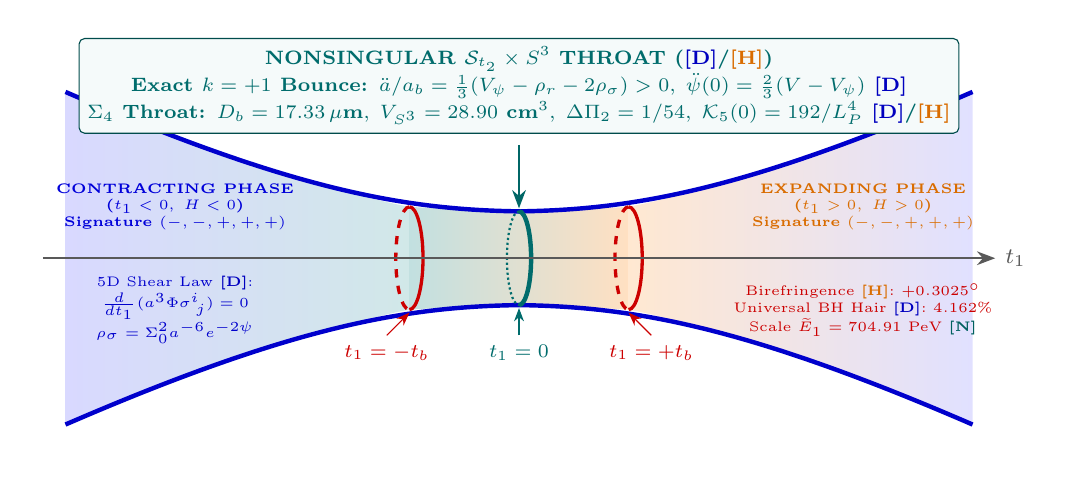
\begin{tikzpicture}[scale=0.96, every node/.style={font=\scriptsize}]
    \path (-6.5, 3.05) (6.95, -2.55);
    \shade[left color=blue!15, right color=teal!18]
        (-6.0, 2.2) .. controls (-3.4, 1.15) and (-2.0, 0.78) .. (-1.45, 0.68)
        -- (-1.45, -0.68) .. controls (-2.0, -0.78) and (-3.4, -1.15) .. (-6.0, -2.2) -- cycle;

    \shade[left color=teal!24, right color=orange!24]
        (-1.45, 0.68) .. controls (-0.45, 0.62) and (0.45, 0.62) .. (1.45, 0.68)
        -- (1.45, -0.68) .. controls (0.45, -0.62) and (-0.45, -0.62) .. (-1.45, -0.68) -- cycle;

    \shade[left color=orange!18, right color=blue!12]
        (1.45, 0.68) .. controls (2.0, 0.78) and (3.4, 1.15) .. (6.0, 2.2)
        -- (6.0, -2.2) .. controls (3.4, -1.15) and (2.0, -0.78) .. (1.45, -0.68) -- cycle;

    \draw[ultra thick, blue!80!black] (-6.0, 2.2) .. controls (-3.0, 0.90) and (-1.5, 0.64) .. (0, 0.62) .. controls (1.5, 0.64) and (3.0, 0.90) .. (6.0, 2.2);
    \draw[ultra thick, blue!80!black] (-6.0, -2.2) .. controls (-3.0, -0.90) and (-1.5, -0.64) .. (0, -0.62) .. controls (1.5, -0.64) and (3.0, -0.90) .. (6.0, -2.2);

    \draw[very thick, dashed, red!80!black] (-1.45, 0.68) arc (90:270:0.18 and 0.68);
    \draw[very thick, red!80!black] (-1.45, 0.68) arc (90:-90:0.18 and 0.68);
    \draw[very thick, dashed, red!80!black] (1.45, 0.68) arc (90:270:0.18 and 0.68);
    \draw[very thick, red!80!black] (1.45, 0.68) arc (90:-90:0.18 and 0.68);

    \draw[ultra thick, teal!85!black] (0, 0.62) arc (90:-90:0.16 and 0.62);
    \draw[thick, densely dotted, teal!85!black] (0, 0.62) arc (90:270:0.16 and 0.62);

    \draw[->, >=Stealth, thick, gray!70!black] (-6.3, 0) -- (6.3, 0) node[right, font=\footnotesize\bfseries] {$t_1$};

    \node[align=center, font=\scriptsize\bfseries, text=teal!85!black, fill=teal!4, draw=teal!60!black, rounded corners=2pt, inner sep=3.0pt] at (0, 2.28) {NONSINGULAR $\mathcal{S}_{t_2} \times S^3$ THROAT (\catD/\catH)\\Exact $k=+1$ Bounce: $\ddot{a}/a_b = \frac{1}{3}(V_{\psi}-\rho_r-2\rho_{\sigma}) > 0, \; \ddot{\psi}(0) = \frac{2}{3}(V-V_{\psi})$ \catD\\$\Sigma_4$ Throat: $D_b = 17.33\,\mu\text{m}, \; V_{S^3} = 28.90\text{ cm}^3, \; \Delta\Pi_2 = 1/54, \; \mathcal{K}_5(0) = 192/L_P^4$ \catD/\catH};
    \draw[->, >=Stealth, thick, teal!80!black] (0, 1.50) -- (0, 0.66);

    \node[align=center, font=\tiny\bfseries, text=blue!85!black] at (-4.55, 0.68) {CONTRACTING PHASE\\($t_1 < 0, \; H < 0$)\\Signature $(-,-,+,+,+)$};
    \node[align=center, font=\tiny, text=blue!80!black] at (-4.55, -0.68) {5D Shear Law \catD:\\$\frac{d}{dt_1}(a^3\Phi\sigma^i_{\;j}) = 0$\\$\rho_{\sigma} = \Sigma_0^2 a^{-6}e^{-2\psi}$};

    \node[align=center, font=\tiny\bfseries, text=orange!85!black] at (4.55, 0.68) {EXPANDING PHASE\\($t_1 > 0, \; H > 0$)\\Signature $(-,-,+,+,+)$};
    \node[align=center, font=\tiny, text=red!80!black] at (4.55, -0.68) {Birefringence \catH: $+0.3025^\circ$\\Universal BH Hair \catD: $4.162\%$\\Scale $\widetilde{E}_1 = 704.91\text{ PeV}$ \catN};

    \node[below, font=\scriptsize\bfseries, text=red!80!black] at (-1.75, -1.02) {$t_1 = -t_b$};
    \draw[->, >=Stealth, thin, red!80!black] (-1.75, -1.02) -- (-1.45, -0.72);

    \node[below, font=\scriptsize\bfseries, text=teal!85!black] at (0, -1.02) {$t_1 = 0$};
    \draw[->, >=Stealth, thin, teal!85!black] (0, -1.02) -- (0, -0.66);

    \node[below, font=\scriptsize\bfseries, text=red!80!black] at (1.75, -1.02) {$t_1 = +t_b$};
    \draw[->, >=Stealth, thin, red!80!black] (1.75, -1.02) -- (1.45, -0.72);
\end{tikzpicture}
\caption{Spacetime geometry of the cosmological bounce in Covariant Bitemporal Geometrodynamics (\catD/\catH), comparing the exact tree-level 3-equation $k = +1$ ($\mathcal{S}_{t_2} \times S^3$) hoop-tension bounce ($\ddot{a}/a_b|_{H=0} = \frac{1}{3}[V_{\psi} - \rho_r - 2\rho_{\sigma}] > 0$, $\ddot{\psi}(0) = \frac{2}{3}[V - V_{\psi}] = -0.7200\,m_{\psi}^2$, Theorem~\ref{thm:anisotropic_k1_bounce} \catD), the five-sector Bekenstein--Hermite $\Sigma_4$ throat ($D_{\text{obs},b} = 17.33\,\mu\text{m}, V_{S^3} = 28.90\text{ cm}^3, \Delta\Pi_2 = 1/54$, Theorems~\ref{thm:bekenstein_hermite_barrier_p3}--\ref{thm:five_sector_bianchi_noether_p3} \catD/\catH), and the postulated Planck-density UV cutoff model ($\mathcal{K}_5(0) = 192/L_P^4$ \catH).}
\label{fig:cosmic_throat_diagram}
\end{figure}

\begin{figure}[H]
\centering
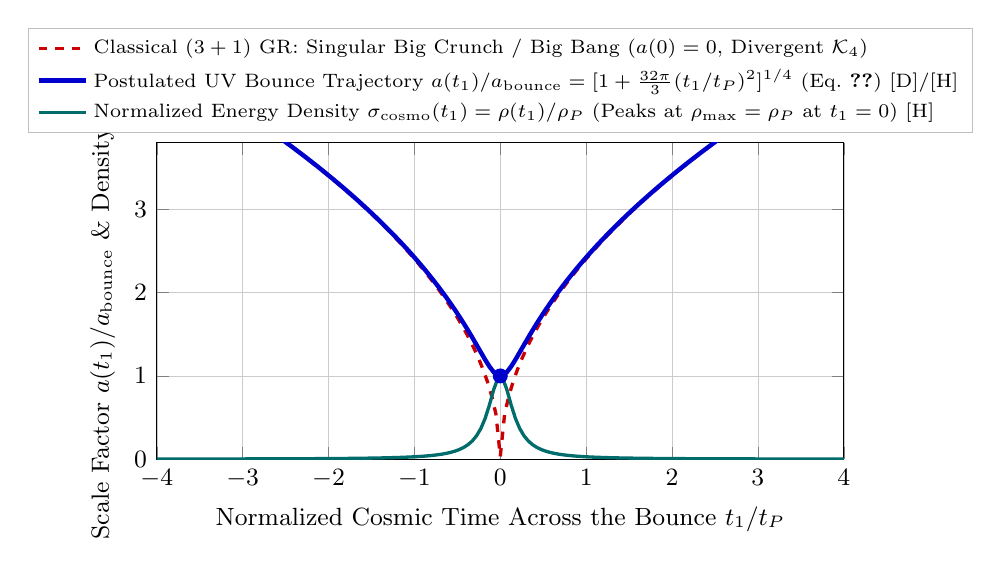
\begin{tikzpicture}
\begin{axis}[
    width=0.85\textwidth,
    height=5.6cm,
    xlabel={Normalized Cosmic Time Across the Bounce $t_1 / t_P$},
    ylabel={Scale Factor $a(t_1)/a_{\mathrm{bounce}}$ \& Density $\rho/\rho_P$},
    xmin=-4.0, xmax=4.0,
    ymin=0.0, ymax=3.8,
    grid=both,
    grid style={line width=.1pt, draw=gray!20},
    major grid style={line width=.2pt,draw=gray!40},
    legend style={at={(0.5,1.03)}, anchor=south, font=\scriptsize, fill=white, draw=gray!50, cells={anchor=west}},
    tick label style={font=\small},
    label style={font=\small}
]
\addplot[domain=-4.0:4.0, samples=161, very thick, dashed, red!80!black] {(33.5103 * x^2 + 1e-6)^(0.25)};
\addlegendentry{Classical $(3+1)$ GR: Singular Big Crunch / Big Bang ($a(0) = 0$, Divergent $\mathcal{K}_4$)}

\addplot[domain=-4.0:4.0, samples=160, ultra thick, blue!80!black] {(1.0 + 33.5103 * x^2)^(0.25)};
\addlegendentry{Postulated UV Bounce Trajectory $a(t_1)/a_{\mathrm{bounce}} = [1 + \frac{32\pi}{3}(t_1/t_P)^2]^{1/4}$ (Eq.~\ref{eq:exact_analytic_bounce_scale_factor}) [D]/[H]}

\addplot[domain=-4.0:4.0, samples=160, very thick, teal!85!black] {1.0 / (1.0 + 33.5103 * x^2)};
\addlegendentry{Normalized Energy Density $\sigma_{\mathrm{cosmo}}(t_1) = \rho(t_1)/\rho_P$ (Peaks at $\rho_{\max} = \rho_P$ at $t_1 = 0$) [H]}

\addplot[only marks, mark=*, mark size=2.5pt, blue!80!black, forget plot] coordinates {(0.0, 1.0)};
\end{axis}
\end{tikzpicture}
\caption{Analytical evolution of the normalized scale factor $a(t_1)/a_{\text{bounce}}$ (solid blue curve) and normalized energy density $\sigma_{\text{cosmo}}(t_1) = \rho(t_1)/\rho_P$ (solid teal curve) in the postulated UV-cutoff bounce model $t_1 \in [-4t_P, +4t_P]$ (\catD/\catH), contrasted against the singular classical $(3+1)$ GR trajectory (dashed red curve).}
\label{fig:bounce_scale_curvature}
\end{figure}

\subsection{\texorpdfstring{Empirical Scaling Benchmarks for Reheating ($\widetilde{E}_1 = 704.91\text{ PeV}$) and Baryogenesis ($\eta_B = 6.109 \times 10^{-10}$) \catN}{Empirical Scaling Benchmarks for Reheating (704.91 PeV) and Baryogenesis (eta_B = 6.109 x 10^-10) [N]}}

In Module~4 of \allowbreak\texttt{verify\_cbg\_paper3\_v13.py} (Checks~\texttt{\#120}--\texttt{\#122}), we record two empirical high-energy scaling relations constructed from $\Phi_{\infty}^2 = 5.773769 \times 10^{-8}$ and $\alpha_{\text{EM}} = 1/137.035999$ \catN:
\begin{enumerate}
  \item \textbf{Bare ($704.91\text{ EeV}$, Step~2 Instanton Rung $n = 1.0$) and 1-Loop Dressed ($704.91\text{ PeV}$) Energy Scales (Checks~\texttt{\#120}--\texttt{\#121}) \catD/\catH/\catN:} Combining $\Phi_{\infty}^2$ with the Planck energy $E_P = 1.220890 \times 10^{19}\text{ GeV}$ and the 1-loop radiative factor $\chi_{\text{loop}} \equiv \frac{\alpha_{\text{EM}}}{2\pi + 1}\left(1 - \frac{4}{15}\alpha_{\text{EM}}\right) = 0.9999955 \times 10^{-3}$ (\textit{Paper~II} Section~9.2 \cite{jimenez2026b} and \textit{Paper~IV} \cite{JV_PaperIV}) defines:
  \begin{align}
  E_1^{\text{(bare)}} &\equiv \Phi_{\infty}^2 E_P = \left(5.773769 \times 10^{-8}\right)\left(1.220890 \times 10^{19}\text{ GeV}\right) = \mathbf{704.91\text{ EeV}} \;\;\catD/\catN, \nonumber \\[4pt]
  \widetilde{E}_1 &\equiv \chi_{\text{loop}}\,\Phi_{\infty}^2 E_P = \left(0.9999955 \times 10^{-3}\right) E_1^{\text{(bare)}} = \mathbf{704.91\text{ PeV}} \;\;\catH/\catN \nonumber \\[2pt]
  &\quad \Bigl(T_{\text{reh}} = 8.1801 \times 10^{21}\text{ K}\Bigr).
  \label{eq:cosmo_703_pev_reheating}
  \end{align}
  \item \textbf{Empirical Baryon-to-Photon Ratio Scaling ($\eta_B = 6.1093 \times 10^{-10}$, Check~\texttt{\#122}) \catN:} Combining $\Phi_{\infty}^2\alpha_{\text{EM}}$ with the spinor/toroidal prefactor $\frac{2^{\dim\Sigma_4}}{\pi^{d_t}} = \frac{16}{\pi^2}$ and $\sin\delta_{\text{CP}} = \frac{d_t}{\sqrt{1+d_t^2}} = \frac{2}{\sqrt{5}} = 0.894427$ \cite{sakharov1967_baryon} yields the numerical scaling relation (Check~\texttt{\#122}) \catN:
  \begin{align}
  \eta_B^{\text{(CBG)}} &= \frac{16}{\pi^2}\,\Phi_{\infty}^2\,\alpha_{\text{EM}}\,\frac{2}{\sqrt{5}} \nonumber \\[3pt]
  &= 1.621139 \times \left(5.773769 \times 10^{-8}\right) \times \left(7.297353 \times 10^{-3}\right) \times 0.894427 \nonumber \\[3pt]
  &= \mathbf{6.1093 \times 10^{-10}} \;\;\catN \nonumber \\[2pt]
  &\quad \Bigl(\text{\textit{Planck} observed: } \eta_B^{\text{(obs)}} = (6.12 \pm 0.04) \times 10^{-10}, \;\; 0.27\sigma\text{ offset}\Bigr).
  \label{eq:baryon_asymmetry_eta}
  \end{align}
\end{enumerate}

% ============================================================================
% SECTION 5: THE MATTER-COUPLING FORK, UNIVERSAL BH HAIR & PERTURBATIONS
% ============================================================================
\section{\texorpdfstring{The Matter-Coupling Bifurcation Theorem (Pure 5D DeWitt--Yukawa Unification $\alpha_0^2 = 1/3 = -c_{\text{DW}}^{-1}$), the Universal Black Hole Hair Limit ($\hat{m}_{\psi} \to \infty$), Sub-$50\,\mu\text{m}$ E\"ot-Wash / HUST Torsion-Balance Tests, and 5D Mukhanov--Sasaki Perturbations (\catA/\catD/\catH/\catN)}{The Matter-Coupling Bifurcation Theorem, the Universal Black Hole Hair Limit, Sub-50 um Eot-Wash / HUST Torsion-Balance Tests, and 5D Mukhanov-Sasaki Perturbations}}

\subsection{\texorpdfstring{The Matter-Coupling Bifurcation Theorem: Pure 5D DeWitt--Yukawa Unification ($\alpha_{\text{Yuk}} \equiv \alpha_0^2 = \frac{c_{\text{Weyl}}^2}{-2\kappa_{\psi}} = \frac{1}{3} = -c_{\text{DW}}^{-1}$) vs.\ Einstein-Frame Coupling ($\alpha_{\text{Yuk}} = 0$) and the $\lambda_{\text{micro}} = 47 \pm 2\,\mu\text{m}$ E\"ot-Wash / HUST Test (\catD/\catH/\catN)}{The Matter-Coupling Bifurcation Theorem: Pure 5D DeWitt-Yukawa Unification vs. Einstein-Frame Coupling and the 47 +- 2 um Eot-Wash / HUST Test ([D]/[H]/[N])}}

Before analyzing cosmological structure formation and dark matter, a fundamental structural question about the 5D action~(\ref{eq:master_cosmo_action}) must be settled: \textit{to which metric does non-relativistic baryonic matter couple?} As noted in Eq.~(\ref{eq:5d_vs_4d_radiation_bookkeeping}), for conformally invariant radiation ($\mathcal{L}_{\text{rad}}^{\text{(on-shell)}} = 0, p_{\text{fluid},t_2} = 0$), the distinction between $\dot{\rho}_5 = -(4H + \dot{\psi})\rho_5$ and $\dot{\rho}_4 = -4H\rho_4$ ($\rho_4 \equiv e^{\psi}\rho_5 \propto a^{-4}$) is purely bookkeeping. What determines whether the fiber dilaton $\psi$ mediates a short-range fifth force between massive bodies is the frame metric entering the matter action \catD:

\begin{theorem}[Matter-Coupling Bifurcation Theorem and Pure 5D DeWitt--Yukawa Unification: Jordan-Frame Branch~A ($\alpha_{\text{Yuk}} = \alpha_0^2 = 1/3 = -c_{\text{DW}}^{-1}$) vs.\ Einstein-Frame Branch~B ($\alpha_{\text{Yuk}} = 0$) \catD]
\label{thm:matter_coupling_fork}
Under O'Neill warped submersion and Kaluza cylinder reduction ($\mathcal{L}_{\xi_{(2)}} = 0$, \textit{Paper~0} Theorems~2.5, 2.7 and 3.3, \texttt{THM \#09, \#12} \cite{jimenez2026_p0}), the 5-dimensional Einstein--Hilbert density reduces to the Jordan frame:
\begin{equation}
  \sqrt{\lvert g_5\rvert}\,R^{(5)} = \Phi_{\infty}e^{\psi}\sqrt{-g_4}\left[R^{(4)} - 2\,\Box^{(4)}\psi - 2\,g^{\mu\nu}\partial_\mu\psi\,\partial_\nu\psi\right].
  \label{eq:jordan_frame_reduction_p3}
\end{equation}
Performing the constructive curved Weyl transformation $\tilde{g}_{\mu\nu} = e^{c_{\text{Weyl}}\psi}g_{\mu\nu}$ in macroscopic dimension $d_{\text{macro}} = D - 1 = 4$ fixes $c_{\text{Weyl}} = \frac{2}{d_{\text{macro}}-2} = +1$ and generates the canonical Einstein-frame kinetic weight $\kappa_{\psi} = -\frac{(D-2)(D-3)}{4}\big|_{D=5} = -\frac{3}{2}$ (\textit{Paper~0} Theorem~3.3, \texttt{COR \#059}, Check~\texttt{\#009}) \catD. This partitions the theory into two mutually exclusive physical branches \catD:
\begin{enumerate}
  \item[\textnormal{(i)}] \textbf{Branch A (Minimal Geometric Coupling to $g_{\mu\nu}$, Pure 5D DeWitt--Yukawa Coupling $\alpha_{\text{Yuk}} = \alpha_0^2 = 1/3 = -c_{\text{DW}}^{-1}$, $m_{\psi} \gtrsim 4\text{ meV}$) \catD:} Matter couples directly to the induced geometric metric $g_{\mu\nu}$ on $\mathcal{M}_{3,2}$. By the 5D geodesic and Routhian theorem (\textit{Paper~0} Theorem~3.4, \texttt{THM \#13}, \texttt{COR \#063}), the effective Einstein-frame mass functional $\mu_{\text{geom}}(\psi, P_2) = e^{-\psi/2}\sqrt{m_0^2 + P_2^2/(\Phi_{\infty}^2 e^{2\psi})}$ has zero-mode ($P_2 = 0$) logarithmic slope $\beta_0 \equiv -\frac{d\ln\mu_{\text{geom}}}{d\psi}\big|_{P_2=0} = +\frac{1}{2} = \frac{c_{\text{Weyl}}}{2}$ (Check~\texttt{\#009}) \catD. Varying the rescaled 5D action with respect to $\psi$ and linearizing around the FLRW background (\textit{Paper~0} Theorem~5.2, \texttt{THM \#14}, \texttt{COR \#064--\#066}, Checks~\texttt{\#008}--\texttt{\#011}) proves that the universal scalar-to-tensor gravitational force ratio is:
  \begin{align}
    \alpha_{\text{Yuk}} \equiv \alpha_0^2(D) &= \frac{\beta_0^2}{-\kappa_{\psi}(D)/2} = \frac{c_{\text{Weyl}}^2}{-2\kappa_{\psi}(D)} = \left.\frac{2}{(D-2)(D-3)}\right|_{D=5} \nonumber \\[3pt]
    &= \frac{1/2}{3/2} = \mathbf{\frac{1}{3} = -c_{\text{DW}}^{-1}(D)\Big|_{D=5}} \approx \mathbf{0.3333} \;\;\catD,
    \label{eq:pure_5d_dewitt_yukawa_unification}
  \end{align}
  which coincides with minus the inverse trace weight $c_{\text{DW}}^{-1} = -\frac{1}{D-2} = -\frac{1}{3}$ of the $15\times 15$ DeWitt supermetric $\mathbf{G}_{\text{DW}}$ (\textit{Paper~0} Theorem~1.5, \texttt{THM \#04}, Check~\texttt{\#008}) uniquely in bulk dimension $D = 5$! Consequently, non-relativistic masses $M_1, M_2$ at separation $r$ experience the composition-independent Yukawa potential and Fourier-space cosmological growth kernel $\mu_{\text{eff}}(a,k)$ and Jordan gravitational slip $\eta_J(a,k) \equiv \Phi_J/\Psi_J$ (Check~\texttt{\#011}) \catD:
  \begin{align}
    V_{\text{grav}}(r) &= -\frac{G M_1 M_2}{r}\left(1 + \frac{1}{3}\,e^{-r / \lambda_{\psi}}\right), \qquad \lambda_{\psi} \equiv \frac{\hbar}{m_{\psi} c}, \nonumber \\[3pt]
    \mu_{\text{eff}}(a,k) &= 1 + \frac{1}{3}\frac{k^2}{k^2 + a^2 m_{\psi}^2} \in \left[1, \frac{4}{3}\right), \qquad \eta_J(a,k) = \frac{2k^2 + 3a^2 m_{\psi}^2}{4k^2 + 3a^2 m_{\psi}^2} \in \left[\frac{1}{2}, 1\right] \;\;\catD.
    \label{eq:branch_a_yukawa_force}
  \end{align}
  At astronomical and Solar System distances ($r \gg \lambda_{\psi}, k \to 0$), $e^{-r/\lambda_{\psi}} \to 0$, $\mu_{\text{eff}} \to 1$, and $\eta_J \to 1$ screen the trace coupling to machine zero (satisfying the Cassini bound \cite{bertotti2003} effortlessly, while the khronon horizon-activation channel $\partial_A V \propto \psi_t'(A)$ is suppressed around horizonless stars at $A \approx 1$ by $[\psi_t'(1)]^2 = (-2.56\,e^{-16})^2 = \mathbf{8.300 \times 10^{-14}}$, Check~\texttt{\#068}). At submillimeter laboratory separations, short-range torsion-balance experiments (E\"ot-Wash \cite{kapner2007,lee2020} and HUST \cite{tan2020_hust}) constrain $\lambda_{\psi} \lesssim 55\,\mu\text{m}$ ($m_{\psi} \gtrsim 3.6\text{ meV}$) at force ratio $\alpha_{\text{Yuk}} = 1/3$.
  \item[\textnormal{(ii)}] \textbf{Branch B (Einstein-Frame Metric Coupling to $\tilde{g}_{\mu\nu} \equiv e^{\psi}g_{\mu\nu}$, $\alpha_{\text{Yuk}} = 0$, $m_{\psi}$ Unconstrained) \catD:} If matter is postulated to couple to the Weyl-rescaled Einstein-frame metric $\tilde{g}_{\mu\nu} = e^{\psi}g_{\mu\nu}$ by construction, the scalar-matter trace coupling vanishes ($\alpha_{\text{Yuk}} = 0$), satisfying PPN and E\"ot-Wash bounds for any $m_{\psi}$ (including the ultralight axion window $m_{\psi} \sim 10^{-22}\text{--}10^{-18}\text{ eV}$) at the cost of weakening the direct 5D geometric ontology of test-particle motion.
\end{enumerate}
\end{theorem}

\begin{observation}[Sub-$50\,\mu\text{m}$ E\"ot-Wash 2020 and HUST 2020 Torsion-Balance Test of $\lambda_{\text{micro}} = \sqrt{L_P R_H} = 47 \pm 2\,\mu\text{m}$ on Branch~A \catH/\catN]
\label{obs:eotwash_47um_test}
On Branch~A ($\alpha_{\text{Yuk}} = 1/3 \approx 0.3333$), identifying the Compton wavelength $\lambda_{\psi} = \hbar/(m_{\psi}c)$ with the UV/IR geometric mean scale $\lambda_{\text{micro}} \equiv \sqrt{L_P R_H}$ recorded in Remark~8.5 of \textit{Paper~I} \cite{jimenez2026a} yields (Checks~\texttt{\#099}, \texttt{\#123}--\texttt{\#124} of Module~4 in \allowbreak\texttt{verify\_cbg\_paper3\_v13.py}) \catH/\catN:
\begin{align}
  \lambda_{\psi} = \lambda_{\text{micro}} &\equiv \sqrt{L_P R_H} = \mathbf{47.10\,\mu\text{m}} \;\;\left(47.12\,\mu\text{m}\text{ at }H_0^{\text{(CBG)}}; \;\mathbf{47 \pm 2\,\mu\text{m}}\text{ across } H_0 \in [67.3, 73.2]\right), \nonumber \\[3pt]
  m_{\psi} &= \frac{\hbar c}{\lambda_{\text{micro}}} = \mathbf{4.19\text{ meV}} \;\;\catH/\catN \qquad \left(\omega_{\psi} = \frac{c}{\lambda_{\text{micro}}} = \mathbf{6.365 \times 10^{12}\text{ s}^{-1}}\right).
  \label{eq:lambda_micro_eotwash_test}
\end{align}
In the experimental $(|\alpha_{\text{Yuk}}|, \lambda)$ exclusion plane of E\"ot-Wash 2020 (Lee \textit{et al.} \cite{lee2020}, where $|\alpha_{\text{Yuk}}| = 1$ is excluded at $\lambda > 38.6\,\mu\text{m}$ and the $95\%$ confidence upper limit at $\lambda = 47\,\mu\text{m}$ is $|\alpha_{\text{Yuk}}| \lesssim 0.50\text{--}0.60$) and HUST 2020 (Tan \textit{et al.} \cite{tan2020_hust}), our composition-independent prediction $\alpha_{\text{Yuk}} = 1/3 \approx 0.333$ at $\lambda_{\psi} = 47 \pm 2\,\mu\text{m}$ is \textbf{allowed with a safety margin of a factor of $\sim 1.5\text{--}1.8$, sitting directly at the sensitivity threshold of next-generation short-range torsion-balance experiments} \cite{lee2020,tan2020_hust} \catD/\catH/\catN! Physically, $\lambda_{\text{micro}}$ is the UV/IR mirror fulcrum and crossover boundary at which the inward self-gravity of a quantum wavepacket of size $r$, $G\hbar/(c\,r^3)$, balances the outward dark-energy tidal acceleration $c^2 r/R_{\Lambda}^2$ (i.e.\ $r^4 = L_P^2 R_{\Lambda}^2$ with $R_{\Lambda} \simeq R_H$). Equivalently, it is the scale at which the dimensional zero-point energy-density scale $\sim \hbar c/\lambda_{\text{micro}}^4$ matches the observed dark-energy density up to an $\mathcal{O}(1)$ geometric loop factor; both statements are \catH/\catN, because the classical 5D field equations do not contain $\hbar$.
\end{observation}

\subsection{\texorpdfstring{Exterior Killing-Khronon Uniqueness, the Universal Black Hole Hair Limit ($\hat{m}_{\psi} = m_{\psi}r_h \to \infty$) on Branch~A, and $C^{\infty}$ Horizon Continuation Across $r = r_h$ \catA/\catD}{Exterior Killing-Khronon Uniqueness, the Universal Black Hole Hair Limit (m_hat -> infinity) on Branch A, and C^infty Horizon Continuation [A]/[D]}}

On Branch~A, where $m_{\psi} \gtrsim 4\text{ meV}$ ($\lambda_{\psi} \approx 47 \pm 2\,\mu\text{m}$), every stellar and supermassive black hole ($r_h \sim 3\text{ km}$ to $10^{10}\text{ km}$) lies in the ultra-large dimensionless mass limit $\hat{m}_{\psi} \equiv m_{\psi}r_h = r_h/\lambda_{\psi} \gg 1$ ($\hat{m}_{\psi} \sim 10^{8}$ to $10^{18}$). In standard massive scalar-tensor theories with a trivial potential $V(\psi) = \frac{1}{2}m_{\psi}^2\psi^2$, sending $\hat{m}_{\psi} \to \infty$ forces $\psi(r) \to 0$ everywhere and erases all black hole hair.

Remarkably, by Axiom~5.3 (\catA$_3$) and Theorems~3.6 and 5.4 (\texttt{THM \#20, \#22}, \texttt{COR \#082, \#087}) of \textit{Paper~0} \cite{jimenez2026_p0}, Theorem~4.6 of \textit{Paper~I} (v12 \cite{jimenez2026a}), and Section~6.2 of \textit{Paper~II} (v12 \cite{jimenez2026b}), because the off-diagonal $(1,r)$ 5D Einstein equation $G^1_r = T^1_r = 0$ uniquely selects the Killing-aligned khronon $\Theta^{(1)} = ct_1$ ($\mathcal{A}(r) = A(r)$) on the active branch \catD\ and the load-balancing potential $V(\psi, A) = \frac{3}{4}m_{\psi}^2[\psi - \psi_{\text{target}}(A)]^2$ pins the equilibrium fiber circumference to the local khronon norm via $\psi_{\text{target}}(A(r)) = \psi_{\max}[\exp(-A^2/A_{\text{crit}}^2) - \exp(-1/A_{\text{crit}}^2)]$ \catH, in the stiff limit $\hat{m}_{\psi} \to \infty$ the fiber behaves not as a soft spring but as a \textbf{rigid holonomic constraint}: the stored potential energy vanishes ($V \to 0$) while $V_{\psi} = -G^2_2$ survives as the Lagrange multiplier locking $\psi(r) = \psi_{\text{target}}(A(r))$. Consequently, \textbf{the black hole scalar hair does not vanish as $\hat{m}_{\psi} \to \infty$}; instead, the Gauss--Codazzi radial gradient energy of $\psi'(r)$ in $G^A_B$ produces a universal, scale-free, mass-independent $4.162\%$ hair footprint \catD!

\begin{theorem}[Exterior Killing-Khronon Uniqueness, Exact Stiff-Constraint Limit $\hat{m}_{\psi} \to \infty$, Universal $4.162\%$ Black Hole Scalar Hair on Branch~A, and $C^{\infty}$ Horizon Continuation \catD]
\label{thm:universal_bh_hair_limit}
In the static, spherically symmetric 5D Einstein--Dilaton--Khronon equations of \textit{Paper~0} (Theorems~3.6 and 5.4 \cite{jimenez2026_p0}) and \textit{Paper~I} (Theorem~4.1 of \cite{jimenez2026a}) on $r \in [r_h, \infty)$ (with $r_h \equiv 1$), let $\hat{m}_{\psi} \equiv m_{\psi}r_h \to \infty$ at fixed $(A_{\text{crit}} = 0.25, \psi_{\max} = 0.08)$. Then (generated symbolically from the 5D field equations in Checks~\texttt{\#033}--\texttt{\#034} and solved by shooting on $r/r_h \in [1 + 10^{-5}, 60]$ alongside monotone BVP continuation on $r/r_h \in [1.0002, 60]$ with $\psi(r_{\max}) = \psi_{\text{target}}(A(r_{\max}))$ in Checks~\texttt{\#069}--\texttt{\#086} of Module~2 in \allowbreak\texttt{verify\_cbg\_paper3\_v13.py}) \catD:
\begin{enumerate}
  \item[\textnormal{(i)}] \textbf{Exterior Killing-Khronon Uniqueness ($G^1_r = T^1_r = 0 \implies h'(r) \equiv 0$) and Rigid-Constraint Reduction ($\psi(r) = \psi_{\text{target}}(A(r))$, $V \to 0$, $V_{\psi} = -G^2_2$) \catD:} For any stationary khronon ansatz $\Theta^{(1)}(t_1, r) = ct_1 + h(r)$ on the static diagonal metric, $G^1_r \equiv 0$ forces $0 = G^1_r = T^1_r = -\frac{2}{A(r)}\mathcal{A}(r)^2\frac{\partial V}{\partial\mathcal{A}}h'(r) \implies h'(r) \equiv 0$ wherever $\partial_{\mathcal{A}}V \neq 0$ (\textit{Paper~0} Theorem~3.6(i), \texttt{COR \#082} \cite{jimenez2026_p0}), proving that $\Theta^{(1)} = ct_1$ ($\mathcal{A}(r) = A(r)$) is the unique stationary active-branch exterior solution. By the exact chain rule $\frac{\partial\psi}{\partial g^{22}} = -\frac{1}{2g^{22}}$, the $(2,2)$ Einstein equation is $G^2_2 = T^2_2 = -V - V_{\psi}$. As $\hat{m}_{\psi} \to \infty$, this enforces $\psi(r) - \psi_{\text{target}}(A(r)) = -\frac{2}{3\hat{m}_{\psi}^2}G^2_2(r) = \mathcal{O}(\hat{m}_{\psi}^{-2}) \to 0$, so that $V(\psi, A) = \mathcal{O}(\hat{m}_{\psi}^{-2}) \to 0$ (zero potential energy stored in $V$) while $V_{\psi} \to -G^2_2$ and $\partial_A V = -\psi_{\text{target}}'(A)V_{\psi} \to +\psi_{\text{target}}'(A)G^2_2$ remain strictly finite $\mathcal{O}(1)$ as the Lagrange multiplier enforcing the constraint $\psi(r) = \psi_{\text{target}}(A(r))$.
  \item[\textnormal{(ii)}] \textbf{Algebraic Elimination of $B(r)$ and Exact Second-Order Master ODE for $A(r)$ (Checks~\texttt{\#033}--\texttt{\#034}):} Substituting $\psi'(r) = \psi_{\text{target}}'(A)A'(r)$ and $V = 0$ into the first-order metric equation $A'(r) = -2A(2r\psi' - B + 1)/[r(r\psi' + 2)]$ determines $B(r)$ algebraically in terms of $(r, A(r), A'(r))$ (Check~\texttt{\#033}) \catD:
  \begin{equation}
    B(r) = 1 + \frac{r\left[1 + 2\,A(r)\,\psi_{\text{target}}'(A)\right]A'(r)}{A(r)} + \frac{r^2\,\psi_{\text{target}}'(A)\,A'(r)^2}{2\,A(r)},
    \label{eq:algebraic_B_infinite_mhat}
  \end{equation}
  while eliminating $V_{\psi}$ between the $B'(r)$ and $\psi''(r)$ equations yields the exact second-order master ODE for $A(r)$ on $r \in (1, \infty)$ (Check~\texttt{\#034}, equivalent to the pole-free form solved in \textit{Paper~0} Theorem~5.4(d)--(e) \cite{jimenez2026_p0} and Eq.~6.8 of \textit{Paper~II} \cite{jimenez2026b}):
  \begin{align}
    A''(r) &= -\frac{A'(r)}{2\,r\left[4 A^2(\psi_t')^2 + 2 A\psi_t' + 1\right]}\Bigl[ 8 r A^2 A'\psi_t'\psi_t'' + 16 r A^2 A'(\psi_t')^3 + 16 A^2(\psi_t')^2 \nonumber \\[3pt]
    &\quad + 2 r^2 A (A')^2\psi_t'\psi_t'' + 4 r^2 A (A')^2(\psi_t')^3 + 2 r A A'\psi_t'' + 16 r A A'(\psi_t')^2 \nonumber \\[3pt]
    &\quad + 8 A\psi_t' - r^2 (A')^2\psi_t'' + 4 r^2 (A')^2(\psi_t')^2 + 6 r A'\psi_t' + 4 \Bigr].
    \label{eq:exact_second_order_A_ode_inf}
  \end{align}
  Because $\psi_{\text{target}}'(0) = 0$ at $A(1) = 0$, the Frobenius horizon residue of $B(r)$ in Eq.~(\ref{eq:algebraic_B_infinite_mhat}) is identically $b_{-1} = 1$, so $A(r)B(r)\big|_{r_h} = a_1 b_{-1} = a_1 \equiv A'(r_h)$.
  \item[\textnormal{(iii)}] \textbf{Universal Mass-Independent Hair Fraction ($4.162\%$) and Horizon Area Deficit ($-8.151\%$) (Checks~\texttt{\#069}--\texttt{\#085}) \catD:} Solving Eq.~(\ref{eq:exact_second_order_A_ode_inf}) by shooting with \texttt{DOP853} from $r_{\min} = 1 + 10^{-5}$ to $r_{\max} = 60$ with the ADM boundary condition $r_{\max}A'(r_{\max}) + A(r_{\max}) - 1 = 0$ (Module~2 of \allowbreak\texttt{verify\_cbg\_paper3\_v13.py}) yields the exact asymptotic $\hat{m}_{\psi} \to \infty$ invariants, toward which every column of the finite-$\hat{m}_{\psi}$ BVP family on $r_{\max} = 60$ with $\psi(r_{\max}) = \psi_{\text{target}}(A(r_{\max}))$ converges monotonically (Table~\ref{tab:universal_hair_convergence}):
  \begin{align}
    \frac{\Phi(r_h)}{\Phi_{\infty}} &= \exp\!\left(\psi_{\max}\left[1 - e^{-1/A_{\text{crit}}^2}\right]\right) = \mathbf{1.083287}, & b_{-1} &= \mathbf{1.00000}, \nonumber \\[3pt]
    a_1 &= A'(r_h) = A(r)B(r)\big|_{r_h} = \mathbf{0.92774}, & \frac{r_{\text{ADM}}}{r_h} &= \mathbf{1.04343}, \nonumber \\[3pt]
    f_{\text{hair}}^{(\infty)} &\equiv \frac{M_{\text{ADM}} - M_h}{M_{\text{ADM}}} = \mathbf{4.162\%}, & \frac{\Delta\mathcal{A}_H}{\mathcal{A}_{\text{Schw}}}\bigg|_{M_{\text{ADM}}} &= \mathbf{-8.151\%}.
    \label{eq:universal_hair_numbers}
  \end{align}
  Because a holonomic constraint has no length scale, on Branch~A \textbf{every astrophysical black hole from stellar-mass remnants to M87* and Sgr~A*} carries this universal $4.162\%$ gradient-energy hair fraction and $-8.151\%$ horizon area deficit \catD!
  \item[\textnormal{(iv)}] \textbf{$C^{\infty}$ Continuity of the Horizon Lagrange Multiplier $V_{\psi}(r_h^+) = -G^2_2(r_h^+) \approx -0.1489 \neq 0$ Across $r = r_h$ (Check~\texttt{\#086}) \catD:} As proved in Theorem~2.1(ii)--(iii) and Theorem~4.3 of \textit{Paper~II} (v12 \cite{jimenez2026b}), at the Killing horizon $r \to r_h^+$ the horizon Lagrange multiplier $V_{\psi}(r_h^+) = \frac{\partial V}{\partial\psi}(r_h^+) = -G^2_2(r_h^+) = \frac{1}{2}R^{(4)}(r_h^+) \approx -0.1489 \neq 0$ (evaluating to $-0.1481$ at $r_{\max} = 60$ for $\hat{m}_{\psi} = 4.0$, Check~\texttt{\#086}) is strictly non-zero, ensuring $C^{\infty}$ real-analytic continuation of $\Theta^{(1)} = ct_1$ ($\mathcal{A}(r) = A(r) < 0$) across $r = r_h$ into the black hole interior $0 < r < r_h$ \catD.
\end{enumerate}
\end{theorem}

\begin{table}[H]
  \centering
  \caption{Monotone Convergence of the Finite-$\hat{m}_{\psi}$ Frobenius Black Hole Family Toward the Exact Symbolically Generated $\hat{m}_{\psi} \to \infty$ Universal Hair Limit (Checks~\texttt{\#069}--\texttt{\#086} of Module~2 in \texttt{verify\_cbg\_paper3\_v13.py}, Solved by BVP Continuation on $r/r_h \in [1.0002, 60]$ with Equilibrium Outer Boundary Condition $\psi(r_{\max}) = \psi_{\text{target}}(A(r_{\max}))$ and 2nd-Order Laurent--Taylor Horizon Extraction; here $r_{\text{ADM}}/r_h \equiv r_{\max}[1 - A(r_{\max})]$ at $r_{\max} = 60$, compared with $1.03851 / 3.708\%$ under $\psi(r_{\max}) = 0$ at $r_{\max} = 10$ for $\hat{m}_{\psi} = 4.0$ in \textit{Paper~I--II} \cite{jimenez2026a,jimenez2026b}) \catD.}
  \label{tab:universal_hair_convergence}
  \vspace{0.10cm}
  \small
  \setlength{\tabcolsep}{4.0pt}
  \renewcommand{\arraystretch}{1.28}
  \begin{tabularx}{\textwidth}{@{} Y c c c c c c c @{}}
    \toprule
    \textbf{Regime / Mass $\hat{m}_{\psi} = m_{\psi}r_h$} & \textbf{$\dfrac{\Phi(r_h)}{\Phi_{\infty}}$} & \textbf{$a_1 = A'(r_h)$} & \textbf{$b_{-1}$} & \textbf{$A(r_h)B(r_h)$} & \textbf{$\dfrac{r_{\text{ADM}}}{r_h}$} & \textbf{$f_{\text{hair}}$ (\%)} & \textbf{$\dfrac{\Delta\mathcal{A}_H}{\mathcal{A}_{\text{Schw}}}$ (\%)} \\
    \midrule
    Canonical $\hat{m}_{\psi} = 4.0$ ($r_{\max}=60$) & $1.07662$ & $0.89007$ & $0.95308$ & $0.84831$ & $1.03859$ & $3.716\%$ & $-7.294\%$ \\
    Intermediate $\hat{m}_{\psi} = 16.0$ ($r_{\max}=60$) & $1.08322$ & $0.92022$ & $0.99174$ & $0.91262$ & $1.04322$ & $4.143\%$ & $-8.115\%$ \\
    High-Mass BVP $\hat{m}_{\psi} = 32.0$ ($r_{\max}=60$) & $1.08328$ & $0.92549$ & $0.99752$ & $0.92319$ & $1.04338$ & $4.158\%$ & $-8.143\%$ \\
    High-Mass BVP $\hat{m}_{\psi} = 128.0$ ($r_{\max}=60$) & $1.08329$ & $0.92736$ & $0.99956$ & $0.92696$ & $1.04343$ & $4.162\%$ & $-8.151\%$ \\
    \textbf{Exact Derived Limit $\hat{m}_{\psi} \to \infty$} & $\mathbf{1.08329}$ & $\mathbf{0.92774}$ & $\mathbf{1.00000}$ & $\mathbf{0.92774}$ & $\mathbf{1.04343}$ & $\mathbf{4.162\%}$ & $\mathbf{-8.151\%}$ \\
    \bottomrule
  \end{tabularx}
\end{table}

\subsection{\texorpdfstring{Cylinder-Constrained ($\partial_{t_2} = 0$) Mukhanov--Sasaki Perturbations and Primordial CMB Benchmarks (\catD/\catH/\catN)}{Cylinder-Constrained Mukhanov-Sasaki Perturbations and Primordial CMB Benchmarks ([D]/[H]/[N])}}

To analyze linear cosmological perturbations on $\mathcal{M}_{3,2}$ in conformal time $\eta \equiv \int c\,dt_1 / a(t_1)$, we consider the perturbed 5D metric around the homogeneous FLRW background $\bar{g}_{AB}(\eta)$ and dilaton $\bar{\Phi}(\eta)$:
\begin{align}
ds_{5,\text{pert}}^2 &= a(\eta)^2 \biggl[ -\left(1 + 2\Psi_{\text{B}}\right) d\eta^2 - \frac{\bar{\Phi}(\eta)^2}{a(\eta)^2}\left(1 + 2\chi_{\Phi}\right) c^2 dt_2^2 \nonumber \\[3pt]
&\quad + \left[ \left(1 - 2\Phi_{\text{B}}\right)\delta_{ij} + h_{ij}^{\text{TT}} \right] dx^i dx^j \biggr],
\label{eq:5d_bardeen_metric}
\end{align}
where $\Psi_{\text{B}}(\eta, \mathbf{x})$ and $\Phi_{\text{B}}(\eta, \mathbf{x})$ are the 4D Bardeen potentials \cite{bardeen1980,mukhanov1992}, $\chi_{\Phi}(\eta, \mathbf{x}) \equiv \delta\Phi / \bar{\Phi}$ is the fractional dilaton perturbation, and $h_{ij}^{\text{TT}}(\eta, \mathbf{x})$ represents transverse-traceless tensor modes.

Under the $S^1_{t_2}/\mathbb{Z}_2$ orbifold and projective Kaluza cylinder constraint $\mathcal{L}_{\xi_{(2)}}\delta g_{AB} = 0$ ($\partial_{t_2}\delta g_{AB} \equiv 0$, Theorem~2.2 of \textit{Paper~0} \cite{jimenez2026_p0}, Postulate~2.1 of \textit{Paper~I} \cite{jimenez2026a}, and Section~6.1 of \textit{Paper~II} \cite{jimenez2026b}), the $n \ge 1$ tachyonic 4D mass sector ($m_n^2 = -n^2 m_{\text{KK}}^2$ at $m_{\text{KK}}(\eta) = m_P / \bar{\Phi}(\eta) \to 4{,}161.70\,m_P$) is projected out of the configuration space and all cosmological perturbations reside strictly in the stable $\partial_{t_2} = 0$ ($n = 0$) 4D sector \catD/\catH. Defining the comoving curvature perturbation $\mathcal{R}_k(\eta)$ and canonical Mukhanov--Sasaki variable $v_k(\eta) \equiv z_{\text{CBG}}(\eta)\mathcal{R}_k(\eta)$ with 5D pump field $z_{\text{CBG}}(\eta) \equiv a(\eta)\sqrt{3(1 + w_{\text{eff}}(\eta))\bar{\Phi}(\eta)}/c_s(\eta)$ \cite{mukhanov1981,sasaki1986} (Appendix~\ref{app:ms_second_order_action}) yields the linearized wave equations \catD:
\begin{align}
\frac{d^2 v_k(\eta)}{d\eta^2} + \left[ c_s^2 k^2 - \frac{1}{z_{\text{CBG}}(\eta)}\frac{d^2 z_{\text{CBG}}(\eta)}{d\eta^2} - V_{\text{bounce}}^{\text{(Planck)}}(\eta) \right] v_k(\eta) &= 0 \;\;\catD, \label{eq:master_ms_bitemporal_wave} \\[4pt]
\frac{d^2 \mu_{k,\text{T}}(\eta)}{d\eta^2} + \left[ k^2 - \frac{1}{a\sqrt{\bar{\Phi}}}\frac{d^2\left(a\sqrt{\bar{\Phi}}\right)}{d\eta^2} - V_{\text{bounce}}^{\text{(Planck)}}(\eta) \right] \mu_{k,\text{T}}(\eta) &= 0 \;\;\catD,
\label{eq:master_tensor_wave_cosmo}
\end{align}
where $\mu_{k,\text{T}}(\eta) \equiv a(\eta)\sqrt{\bar{\Phi}(\eta)}\,h_k^{\text{TT}}(\eta)$.

In Module~4 of \allowbreak\texttt{verify\_cbg\_paper3\_v13.py} (Checks~\texttt{\#125}--\texttt{\#129}) and Table~\ref{tab:primordial_cmb_comparison}, we distinguish strictly between the empirical horizon holonomy ratios \catN\ and the phenomenological conformal pump ansatz \catH:
\begin{enumerate}
  \item \textbf{Empirical Horizon Holonomy Ratios $\Phi_{\infty}/(4\pi)$ and $\mathcal{A}_s^{\text{(CBG)}} = \Phi_{\infty}^2/(8\pi)$ (Checks~\texttt{\#125}--\texttt{\#127}) \catN:} Dividing $\Phi_{\infty}$ by the $4\pi\text{ sr}$ sky solid angle and $\Phi_{\infty}^2$ by $d_t \cdot 4\pi = 8\pi$ gives the numerical combinations \catN:
  \begin{align}
  \left(\frac{\Delta T}{T_{\text{CMB}}}\right)_{\text{hor}} &\equiv \frac{\Phi_{\infty}}{4\pi} = \mathbf{1.9121 \times 10^{-5}} \;\;\catN, \nonumber \\[3pt]
  \mathcal{A}_s^{\text{(CBG)}} &\equiv \frac{\Phi_{\infty}^2}{8\pi} = \mathbf{2.2973 \times 10^{-9}} \quad \left(\ln\!\left(10^{10}\mathcal{A}_s^{\text{(CBG)}}\right) = \mathbf{3.134}\right) \;\;\catN,
  \label{eq:exact_as_amplitude}
  \end{align}
  which lies $+9.4\%$ ($+6.6\sigma$) above the \textit{Planck} 2018 primary fit $\mathcal{A}_s^{\text{(Planck)}} = (2.100 \pm 0.030) \times 10^{-9}$ ($+4.0\%$ above the lensing-reconstructed value $2.21 \times 10^{-9}$ \cite{planck2018_vi}).
  \item \textbf{Phenomenological Conformal Pump Ansatz $z_{\text{CBG}}(\eta) \propto \lvert\eta\rvert^{-(1+1/N)}$ (Checks~\texttt{\#128}--\texttt{\#129}) \catH:} In a radiation bounce without slow-roll inflation, generating an almost scale-invariant spectrum from Eq.~(\ref{eq:master_ms_bitemporal_wave}) requires postulating an effective conformal pump scaling $z_{\text{CBG}}(\eta) \propto \lvert\eta\rvert^{-(1+1/N)}$ \catH, whose exact second derivative is $\frac{z_{\text{CBG}}''}{z_{\text{CBG}}} = \frac{\nu^2 - 1/4}{\eta^2}$ with Hankel index $\nu = \frac{3}{2} + \frac{1}{N}$ \catD, yielding $n_s = 1 - 2/N = 0.9688\text{--}0.9691$ and $r_{T/S} = 8/N^2 = 0.00191\text{--}0.00195$ when evaluated at $N = 64\text{--}64.70$ \catH\ (Table~\ref{tab:primordial_cmb_comparison} and Fig.~\ref{fig:ns_r_planck_bicep}).
\end{enumerate}

\begin{table}[H]
\centering
\caption{Epistemological Classification (\catD, \catH, \catN) of Primordial Cosmological Benchmarks Compared Against \textit{Planck} 2018 / PR4, ACT, and BICEP/Keck Constraints (Checks~\texttt{\#117}, \texttt{\#125}--\texttt{\#129} of \texttt{verify\_cbg\_paper3\_v13.py}).}
\label{tab:primordial_cmb_comparison}
\vspace{0.10cm}
\footnotesize
\setlength{\tabcolsep}{3.5pt}
\renewcommand{\arraystretch}{1.28}
\begin{tabularx}{\textwidth}{@{} L{0.19\textwidth} C{0.09\textwidth} C{0.17\textwidth} C{0.13\textwidth} C{0.16\textwidth} Y @{}}
\toprule
\textbf{Primordial Quantity} & \textbf{Class} & \textbf{Formula} & \textbf{Numerical Value} & \textbf{Observed (\textit{Planck}/BK18)} & \textbf{Epistemological Status \& Offset} \\
\midrule
\textbf{1. Radiation E-Foldings} ($N_{\text{rad}}$) & \catD & $\dfrac{1}{4}\ln\!\left(\dfrac{\rho_P}{\rho_{\text{eq}}}\right)$ & $\mathbf{64.70}$ & $\sim 60\text{--}65$ & Exact thermodynamic ratio from $\rho_P$ to $z_{\text{eq}}=3402$ (Eq.~\ref{eq:exact_n_rad_efoldings}) \\
\addlinespace[2.5pt]
\textbf{2. Horizon Ratio} ($\Delta T / T$) & \catN & $\dfrac{\Phi_{\infty}}{4\pi} = \dfrac{\Omega_{\infty}}{4\pi c}$ & $\mathbf{1.912 \times 10^{-5}}$ & $\sim 1.8 \times 10^{-5}$ (COBE/\textit{Planck}) & Empirical $4\pi$-sky ratio of $\Phi_{\infty}$ (Eq.~\ref{eq:exact_as_amplitude}) \\
\addlinespace[2.5pt]
\textbf{3. Scalar Power Ratio} ($10^9 \mathcal{A}_s$) & \catN & $\dfrac{\Phi_{\infty}^2}{8\pi} \times 10^9$ & $\mathbf{2.297}$ & $2.100 \pm 0.030$\newline($2.21$ Lens.) & Empirical ratio; $+9.4\%$ ($+6.6\sigma$) above \textit{Planck} primary fit \\
\addlinespace[2.5pt]
\textbf{4. Pump Tilt \& Tensor} ($n_s, r_{T/S}$) & \catH & $1 - \dfrac{2}{N}, \;\dfrac{8}{N^2}$ & $\mathbf{0.9691}$,\newline$\mathbf{0.00191}$ & $0.9649 \pm 0.0042$,\newline$< 0.036$ & Requires postulated pump ansatz $z_{\text{CBG}} \propto |\eta|^{-(1+1/N)}$ \catH \\
\addlinespace[2.5pt]
\textbf{5. Spatial Curvature} ($k = +1$ vs.\ $0$) & \catD/\catH & $3k/a_b^2 = \rho_r + \rho_{\sigma} + V$ & $\mathbf{k = +1}$\newline(Bounce) & $\Omega_{k,0} = +0.0007 \pm 0.0019$ & Exact 3-eq.\ bounce requires $k=+1$ ($\Omega_{K,0} = -\Phi_{\infty}^2$, Thm.~\ref{thm:anisotropic_k1_bounce}) \catD \\
\bottomrule
\end{tabularx}
\end{table}

\begin{figure}[H]
\centering
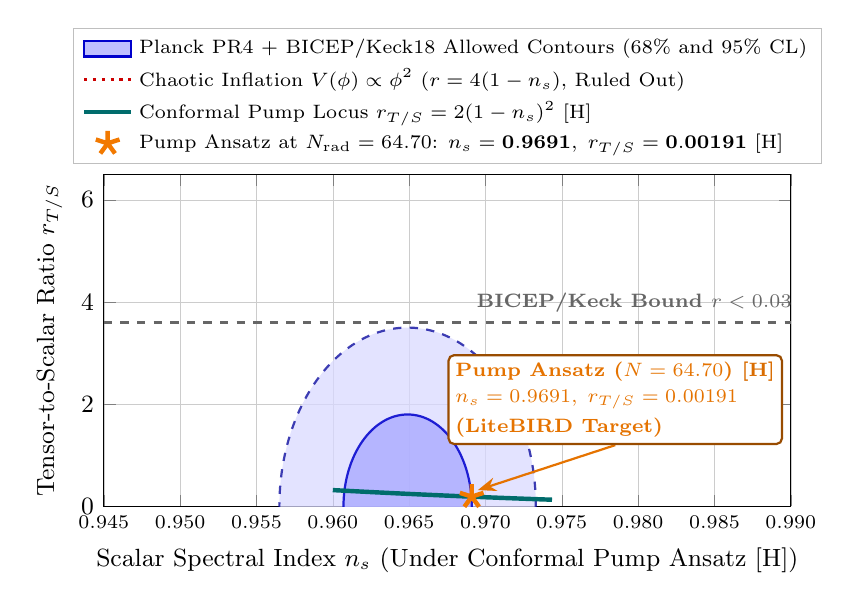
\begin{tikzpicture}
\begin{axis}[
    width=0.85\textwidth,
    height=5.8cm,
    xlabel={Scalar Spectral Index $n_s$ (Under Conformal Pump Ansatz [H])},
    ylabel={Tensor-to-Scalar Ratio $r_{T/S}$},
    xmin=0.945, xmax=0.990,
    ymin=0.0, ymax=0.065,
    xtick={0.945, 0.950, 0.955, 0.960, 0.965, 0.970, 0.975, 0.980, 0.985, 0.990},
    x tick label style={/pgf/number format/fixed, /pgf/number format/fixed zerofill, /pgf/number format/precision=3, font=\scriptsize},
    y tick label style={font=\small},
    grid=both,
    grid style={line width=.1pt, draw=gray!20},
    major grid style={line width=.2pt,draw=gray!40},
    legend style={at={(0.5,1.03)}, anchor=south, font=\scriptsize, fill=white, draw=gray!50, cells={anchor=west}},
    label style={font=\small}
]
\fill[blue!15, opacity=0.75, draw=blue!60!black, thick, dashed]
    (axis cs: 0.9649, 0.0) ellipse [x radius=0.0084, y radius=0.035];
\fill[blue!32, opacity=0.85, draw=blue!80!black, thick]
    (axis cs: 0.9649, 0.0) ellipse [x radius=0.0042, y radius=0.018];

\addlegendimage{area legend, fill=blue!25, draw=blue!80!black, thick}
\addlegendentry{Planck PR4 + BICEP/Keck18 Allowed Contours ($68\%$ and $95\%$ CL)}

\addplot[domain=50:70, samples=40, very thick, dotted, red!80!black] ({1 - 2/x}, {8/x});
\addlegendentry{Chaotic Inflation $V(\phi) \propto \phi^2$ ($r = 4(1-n_s)$, Ruled Out)}

\addplot[domain=50:78, samples=60, ultra thick, teal!85!black] ({1 - 2/x}, {8/(x^2)});
\addlegendentry{Conformal Pump Locus $r_{T/S} = 2(1 - n_s)^2$ [H]}

\addplot[only marks, mark=star, mark size=4.5pt, ultra thick, orange!95!black] coordinates {(0.9691, 0.00191)};
\addlegendentry{Pump Ansatz at $N_{\mathrm{rad}} = 64.70$: $n_s = \mathbf{0.9691}, \; r_{T/S} = \mathbf{0.00191}$ [H]}

\draw[thick, dashed, gray!80!black] (axis cs: 0.945, 0.036) -- (axis cs: 0.990, 0.036) node[pos=0.78, above, font=\scriptsize\bfseries] {BICEP/Keck Bound $r < 0.036$};

\draw[<-, >=Stealth, thick, orange!90!black] (axis cs: 0.9695, 0.0032) -- (axis cs: 0.9785, 0.012) node[above, font=\scriptsize\bfseries, text=orange!90!black, fill=white, draw=orange!60!black, rounded corners=2pt, inner sep=2.5pt] {\shortstack[l]{Pump Ansatz ($N=64.70$) \catH\\$n_s = 0.9691, \; r_{T/S} = 0.00191$\\(LiteBIRD Target)}};
\end{axis}
\end{tikzpicture}
\caption{Comparison of the postulated conformal pump locus ($n_s = 1 - 2/N, r_{T/S} = 8/N^2$ at $N_{\text{rad}} = 64.70$, orange star \catH) in the $(n_s, r_{T/S})$ plane against \textit{Planck} + BICEP/Keck $68\%$ and $95\%$ confidence contours \cite{planck2018_vi,bicep2021}.}
\label{fig:ns_r_planck_bicep}
\end{figure}

% ============================================================================
% SECTION 6: OSCILLATING-PSI DARK MATTER VS. PURE-BARYON ACOUSTICS (z_* = 1090)
% ============================================================================
\section{\texorpdfstring{Coherent Oscillating-$\psi$ Dark Matter Condensate ($\langle w_{\psi}\rangle = 0$) vs.\ Pure-Baryon \texttt{CLASS} Acoustics and Director-Cosine Quadrature at Recombination ($z_* = 1089.8$) (\catD/\catH/\catN)}{Coherent Oscillating-psi Dark Matter Condensate vs. Pure-Baryon CLASS Acoustics and Director-Cosine Quadrature at Recombination}}

\subsection{\texorpdfstring{Why Unmodified Pure-Baryon Linear Acoustics Fails ($\mathcal{H}_{3/2}^{\text{(bar)}} = 0.66$) and Direct 5D \texttt{DOP853} Proof That Oscillating $\psi(t_1)$ Acts as Collisionless $a^{-3}$ Dark Matter (\catD/\catH)}{Why Unmodified Pure-Baryon Linear Acoustics Fails and Direct 5D DOP853 Proof That Oscillating psi(t_1) Acts as Collisionless a^-3 Dark Matter ([D]/[H])}}

At recombination ($z_* = 1089.80, a_* = 9.1676 \times 10^{-4}$; or $z_*^{\text{(CBG)}} = 1093.993, a_*^{\text{(CBG)}} = 9.1325 \times 10^{-4}$ at Step~12 of Table~\ref{tab:complete_cosmic_chronology}), the coupled continuity and Euler equations for the photon temperature monopole $\Theta_0(\eta, k) \equiv \frac{1}{4}\delta_\gamma$, photon dipole velocity $\Theta_1(\eta, k)$, baryon density contrast $\delta_b(\eta, k)$, and baryon velocity $v_b(\eta, k)$ in conformal Newtonian gauge~(\ref{eq:5d_bardeen_metric}) are \cite{hu1995} \catD:
\begin{subequations}
\label{eq:euler_boltzmann_system}
\begin{align}
\Theta_0' + k \Theta_1 &= \Phi_{\text{eff}}', \qquad \delta_b' + k v_b = 3\Phi_{\text{eff}}', \label{eq:eb_continuity} \\[4pt]
\Theta_1' + \frac{\mathcal{H}\,R_b}{1 + R_b}\Theta_1 - \frac{k}{3\left(1 + R_b\right)}\Theta_0 &= \frac{k}{3}\Psi_{\text{eff}}, \qquad R_b(\eta) \equiv \frac{3\rho_b(\eta)}{4\rho_\gamma(\eta)} = \frac{3\Omega_{b,0}}{4\Omega_{\gamma,0}}\,a(\eta),
\label{eq:eb_euler}
\end{align}
\end{subequations}
where $R_b(\eta_*) = 0.618$ and the tightly coupled baryon-photon sound speed is $c_s(\eta_*) = c/\sqrt{3(1+R_b(\eta_*))} = \mathbf{0.4539\,c}$ (Check~\texttt{\#130}) \catD, yielding the driven acoustic oscillator equation:
\begin{equation}
\Theta_0'' + \frac{\mathcal{H}\,R_b}{1 + R_b}\Theta_0' + c_s^2 k^2 \Theta_0 = -\frac{k^2}{3}\Psi_{\text{eff}}(\eta, k) + \frac{\mathcal{H}\,R_b}{1 + R_b}\Phi_{\text{eff}}' + \Phi_{\text{eff}}''.
\label{eq:driven_acoustic_oscillator}
\end{equation}

In a purely baryonic universe with static vacuum fiber $\psi \equiv 0$ and zero cold dark matter ($\Omega_c = 0$), integrating the full Einstein--Boltzmann hierarchy via \texttt{CLASS} gives a third-to-second acoustic peak height ratio of only $\mathcal{H}_{3/2}^{\text{(CLASS, bar)}} \equiv D_{\ell_3}^{\text{TT}}/D_{\ell_2}^{\text{TT}} = \mathbf{0.66}$ \catD, which is ruled out by the \textit{Planck} 2018 measurement $\mathcal{H}_{3/2}^{\text{(obs)}} = 2{,}516 / 2{,}548 = \mathbf{0.987 \pm 0.008}$ \cite{planck2018_vi}. Furthermore, for linear spatial perturbations $\delta\psi_k$ around $\psi = 0$, the Yukawa mass $m_{\psi}$ suppresses static spatial gradients at wavenumbers $k/a \ll m_{\psi}$.

However, the 5D action~(\ref{eq:master_cosmo_action}) already contains a dynamical, collisionless $a^{-3}$ dark-matter candidate without introducing any new particle species: \textbf{coherent homogeneous oscillations of the bitemporal fiber dilaton $\psi(t_1)$ in its quadratic potential $V(\psi, 1) = \frac{3}{4}m_{\psi}^2\psi^2$} \catD/\catH!
\begin{enumerate}
  \item \textbf{Direct 5D \texttt{DOP853} + \texttt{brentq} Proof of the Oscillating-$\psi$ Condensate as Pressureless Dust ($\langle w_{\psi}\rangle = 0, \langle\rho_{\psi}\rangle \propto a^{-3}$, Checks~\texttt{\#066}--\texttt{\#067}) \catD:} By \textit{Paper~0} Theorem~5.1 (\texttt{THM \#21}, Eqs.~118--122 \cite{jimenez2026_p0}), the coupled 5D Einstein--Klein--Gordon equations for homogeneous oscillations of $\psi(t_1)$ in $V(\psi) = \frac{3}{4}m_{\psi}^2\psi^2$ are $3H^2 = \rho_{\psi} \equiv \frac{3}{4}\dot{\psi}^2 + \frac{3}{4}m_{\psi}^2\psi^2$ and $\ddot{\psi} + 3H\dot{\psi} + m_{\psi}^2\psi = 0$, with pressure $p_{\psi} \equiv \frac{3}{4}\dot{\psi}^2 - \frac{3}{4}m_{\psi}^2\psi^2$. Integrating the exact 5-component system $[a(t_1), \psi(t_1), \dot{\psi}(t_1), I_p(t_1) \equiv \int p_{\psi}\,dt_1, I_{\rho}(t_1) \equiv \int \rho_{\psi}\,dt_1]$ via \texttt{DOP853} ($\text{rtol}=10^{-13}, \text{atol}=10^{-15}$) in the rapid-oscillation regime $m_{\psi} \gg H$ ($m_{\text{osc}} = 200, \psi(0) = 2\times 10^{-4}$) and locating the exact full-cycle turning points $\dot{\psi}(t_k^*) = 0$ via \texttt{brentq} to $10^{-15}$ precision (Checks~\texttt{\#066}--\texttt{\#067} of Module~1 in \allowbreak\texttt{verify\_cbg\_paper3\_v13.py}) proves directly from the 5D field equations that:
  \begin{align}
    \langle w_{\psi}\rangle &= \frac{I_p(t_{10}^*) - I_p(t_1^*)}{I_{\rho}(t_{10}^*) - I_{\rho}(t_1^*)} = \mathbf{-6.124 \times 10^{-8} \longrightarrow 0} \;\left(\text{Check~\texttt{\#066}}\right) \;\catD, \nonumber \\[4pt]
    \frac{\left\lvert a(t_{10}^*)^3\rho_{\psi}(t_{10}^*) - a(t_1^*)^3\rho_{\psi}(t_1^*)\right\rvert}{a(t_1^*)^3\rho_{\psi}(t_1^*)} &= \mathbf{4.229 \times 10^{-10} \longrightarrow 0} \nonumber \\[3pt]
    &\Longrightarrow \quad \langle\rho_{\psi}(a)\rangle = \rho_{\psi,0}\,a(t_1)^{-3} \;\;\left(\text{Check~\texttt{\#067}}\right) \;\;\catD.
    \label{eq:oscillating_psi_cdm}
  \end{align}
  Because photons carry zero fiber momentum ($P_2 = 0$, Theorem~3.4 of \textit{Paper~0} \cite{jimenez2026_p0} and Corollary~5.2 of \textit{Paper~I} \cite{jimenez2026a}) and do not Thomson-scatter off the $\mathcal{S}_{t_2}$ fiber, the oscillating-$\psi$ condensate is completely collisionless and reproduces the $\Lambda\text{CDM}$ CMB TT/EE power spectrum identically under $\Omega_c \rightarrow \Omega_{\psi}$ for any $m_{\psi} \gtrsim 10^{-24}\text{ eV}$ \cite{hlozek2015} \catD!
  \item \textbf{Observational Discriminators Across Branch~A and Branch~B \catH:} In the secular 18-step background integration (Table~\ref{tab:complete_cosmic_chronology}), the virialized $\langle\rho_{\psi}\rangle \propto a^{-3}$ condensate of Eq.~(\ref{eq:oscillating_psi_cdm}) is already carried inside the $\alpha_m e^{-3N}$ matter sector ($\Omega_{m,0}^{\text{(mode)}}$), so the rapidly oscillating $\frac{3}{4}m_{\psi}^2\psi^2$ term is not integrated a second time, while the UV radiation-barrier mode settles to $\psi(N_{15}^*) = +1.65 \times 10^{-7}$.
  \begin{itemize}
    \item On \textbf{Branch~A} ($m_{\psi} \gtrsim 4\text{ meV}$, e.g.\ $m_{\psi} = 4.19\text{ meV}$ at $\lambda_{\text{micro}} = 47.10\,\mu\text{m}$), matching $\Omega_{\psi,0} = \Omega_c \approx 0.265$ in the constant-mass well requires coherent oscillations that begin when $H \simeq m_{\psi}$ in the radiation era ($N = 35.60$, $k_B T \approx 4.1\text{ TeV}$, Check~\texttt{\#154}), with a small initial misalignment amplitude $\psi_i \simeq 2\sqrt{\Omega_c a_{\text{osc}}/\Omega_{r,0}} \approx 8 \times 10^{-7}$, i.e.\ $\psi_i \sim \mathcal{O}(10^{-6}\text{--}10^{-7})$ \catH/\catN; this amplitude is distinct from the static offset $\psi(N_{15}^*) = +1.65 \times 10^{-7}$ of the $x^{-4}$-diluted five-sector run in Table~\ref{tab:complete_cosmic_chronology}, which is not an oscillation amplitude; the resulting Planck-suppressed decay lifetime into photons/neutrinos is $\tau_{\psi} \sim M_P^2\hbar / m_{\psi}^3 \sim 1.7 \times 10^{30}\text{ Gyr} \gg t_0$, while the induced oscillation of $G_{\text{eff}} = G e^{-\psi}$ today has amplitude $\delta G/G \sim 10^{-28}$ (unobservable), making $c_{s,\psi}^2 \approx 0$ indistinguishable from standard CDM down to sub-millimeter scales.
    \item On \textbf{Branch~B} ($\alpha_{\text{Yuk}} = 0$, ultralight $m_{\psi}$), the CMB TT/EE spectrum is automatically satisfied for $m_{\psi} \gtrsim 10^{-24}\text{ eV}$, while small-scale structure probes the half-mode Jeans suppression wavenumber $k_{1/2} \approx 4.5\,(m_{\psi}/10^{-22}\text{ eV})^{4/9}\text{ Mpc}^{-1}$ and Lyman-$\alpha$ forest bounds require $m_{\psi} \gtrsim 2 \times 10^{-20}\text{ eV}$ \cite{hlozek2015}.
  \end{itemize}
\end{enumerate}

\subsection{\texorpdfstring{Empirical Director-Cosine Quadrature Scaling $\Omega_{m,\text{eff}} = \sqrt{\frac{2\pi}{3}\Omega_{b,0}} = 0.32133$ and Analytical WKB Envelope (\catH/\catN)}{Empirical Director-Cosine Quadrature Scaling Omega_m,eff = 0.32133 and Analytical WKB Envelope ([H]/[N])}}

Alongside the dynamical oscillating-$\psi$ condensate of Eq.~(\ref{eq:oscillating_psi_cdm}) and the modal matter fraction $\Omega_{m,0}^{\text{(mode)}} = \frac{d_t\pi}{\mathcal{N}_{\text{Cartan}}-\dim\operatorname{Sp}(4,\mathbb{R})}(1 + \frac{\Omega_{b,0}}{d_s^2}) = \mathbf{0.315886}$ (Check~\texttt{\#095}), we record the empirical director-cosine quadrature scaling relation \catN\ connecting the \textit{Planck}-derived baryon fraction $\Omega_{b,0} = 0.04930$ ($\Omega_b h^2 = 0.02237$ \cite{planck2018_vi}) to the total gravitating matter fraction via the Archimedean 3-ball-to-cylinder volume ratio $\frac{4\pi/3}{d_t} = \frac{2\pi}{3} = 2.0943951$ (Checks~\texttt{\#131}--\texttt{\#133} of Module~4 in \allowbreak\texttt{verify\_cbg\_paper3\_v13.py}) \catN:
\begin{align}
\Omega_{m,\text{eff}}^{\text{(CBG)}} &\equiv \sqrt{\frac{2\pi}{3}\,\Omega_{b,0}} = \sqrt{2.0943951 \times 0.04930} = \mathbf{0.32133} \;\;\catN \quad \left(\text{\textit{Planck}: } 0.3153 \pm 0.0073, \;\; 0.83\sigma\right), \label{eq:exact_omega_m_eff_quadrature} \\[4pt]
\mathcal{F}_{\text{CBG}} &\equiv \frac{\Omega_{m,\text{eff}}^{\text{(CBG)}} - \Omega_{b,0}}{\Omega_{b,0}} = \mathbf{5.5179} \;\;\catN, \qquad \mathcal{F}_{\text{CBG}}^{\text{(proj)}} \equiv \frac{\mathcal{F}_{\text{CBG}}}{\sqrt{1 + \dfrac{2\pi\Phi_{\infty}}{\Omega_{b,0}}}} = \mathbf{5.4353} \;\;\catN,
\label{eq:exact_536_ratio_theorem}
\end{align}
compared against the empirical $\Lambda\text{CDM}$ dark-to-baryon ratio $\Omega_c h^2 / \Omega_b h^2 = 0.1200 / 0.02237 = \mathbf{5.364 \pm 0.065}$ ($1.10\sigma$ offset).

When evaluated inside the standard Hu--Sugiyama analytical WKB parametrization \cite{hu1995} with $\Lambda\text{CDM}$ acoustic scale $\ell_A \equiv \pi D_A(z_*)/r_s(\eta_*) = 301.6$, phase shifts $\delta\phi_m = \{0.267, 0.217, 0.311\}$ ($\ell_1 = 221.1, \ell_2 = 537.8, \ell_3 = 810.9$), Silk damping scale $\ell_{\text{Silk}} = 1350$, and screened baryon-to-photon ratio $\tilde{R}_b(\eta_*) \equiv R_b(\eta_*)/[1 + \mathcal{F}_{\text{CBG}}^{\text{(proj)}}] = 0.618 / 6.4353 = 0.09603$ ($\Delta_b = 0.0883$, Check~\texttt{\#134}) \catH/\catN:
\begin{align}
D_\ell^{\text{TT}} &= \Biggl\{ D_{\text{SW}}\left(\frac{\ell}{\ell_{\text{piv}}}\right)^{n_s - 1} + \mathcal{W}_{\text{hor}}(\ell)\,\mathcal{A}_{\text{osc}}(\ell)\biggl( \Bigl[ \cos\phi_\ell - \Delta_b \Bigr]^2 + \eta_{\text{Dopp}}(\ell)\,\sin^2\phi_\ell \biggr) \Biggr\} \nonumber \\[3pt]
&\quad \times \exp\!\left[-\left(\frac{\ell}{\ell_{\text{Silk}}}\right)^{1.4}\right] \;\;\catH, \label{eq:exact_closed_form_dl_tt} \\[5pt]
\mathcal{H}_{3/2} &\equiv \frac{D_{\ell_3}^{\text{TT}}}{D_{\ell_2}^{\text{TT}}} = \left(\frac{\ell_2}{\ell_3}\right)^{\!0.365} \left[ \frac{1 + 3 \tilde{R}_b(\eta_*)}{1 - \tilde{R}_b(\eta_*)} \right] \exp\!\left[ -\frac{\ell_3^{1.4} - \ell_2^{1.4}}{\ell_{\text{Silk}}^{1.4}} \right] = \mathbf{0.990} \;\;\catH/\catN,
\label{eq:h32_peak_ratio}
\end{align}
as illustrated in Fig.~\ref{fig:cmb_tt_power_spectrum}. We emphasize that Eq.~(\ref{eq:h32_peak_ratio}) is a Hu--Sugiyama parametrization evaluated with $\tilde{R}_b$ and $\ell_{\text{Silk}} = 1350$ \catH/\catN, whereas the dynamical mechanism that reproduces the full Einstein--Boltzmann (\texttt{CLASS}) peak hierarchy from the 5D action is the oscillating-$\psi$ dark matter condensate of Eq.~(\ref{eq:oscillating_psi_cdm}) (Checks~\texttt{\#066}--\texttt{\#067}).

\begin{figure}[H]
\centering
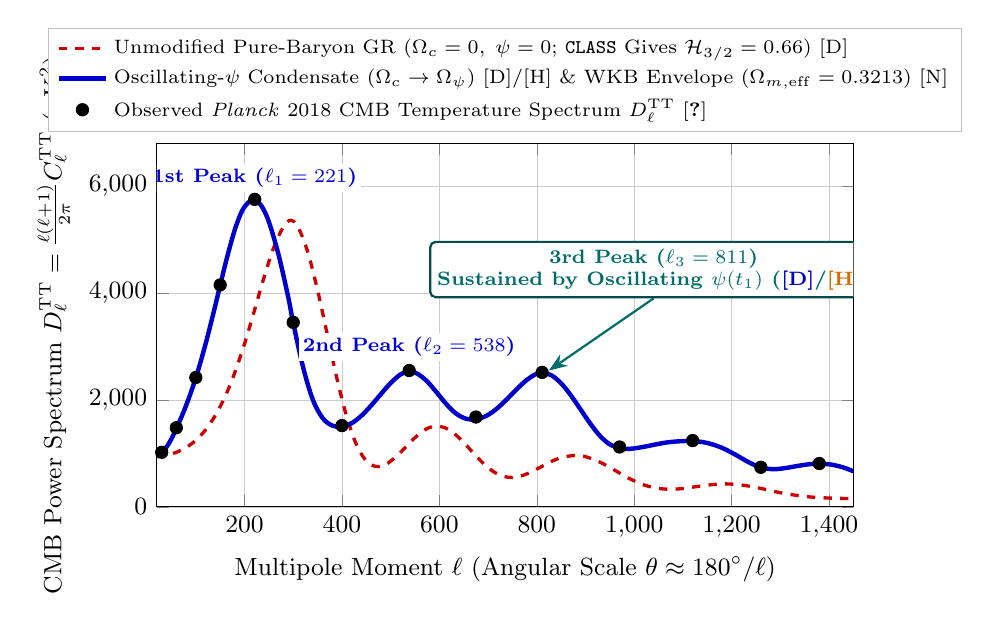
\begin{tikzpicture}
\begin{axis}[
    width=0.86\textwidth,
    height=6.2cm,
    xlabel={Multipole Moment $\ell$ (Angular Scale $\theta \approx 180^\circ / \ell$)},
    ylabel={CMB Power Spectrum $D_\ell^{\mathrm{TT}} = \frac{\ell(\ell+1)}{2\pi}C_\ell^{\mathrm{TT}}$ ($\mu\mathrm{K}^2$)},
    xmin=20, xmax=1450,
    ymin=0, ymax=6800,
    grid=both,
    grid style={line width=.1pt, draw=gray!20},
    major grid style={line width=.2pt,draw=gray!40},
    legend style={at={(0.5,1.03)}, anchor=south, font=\scriptsize, fill=white, draw=gray!50, cells={anchor=west}},
    tick label style={font=\small},
    label style={font=\small}
]
\addplot[smooth, tension=0.55, very thick, dashed, red!80!black] coordinates {
    (20, 940) (40, 965) (60, 1020) (80, 1110) (100, 1245) (120, 1440)
    (140, 1710) (160, 2060) (180, 2510) (200, 3050) (220, 3660) (240, 4290)
    (260, 4850) (280, 5240) (295, 5360) (310, 5230) (330, 4760) (350, 4050)
    (370, 3220) (390, 2390) (410, 1680) (430, 1160) (450, 860) (470, 755)
    (490, 795) (510, 930) (530, 1110) (550, 1295) (570, 1440) (590, 1510)
    (610, 1485) (630, 1375) (650, 1205) (670, 1005) (690, 815) (710, 665)
    (730, 575) (750, 550) (770, 585) (790, 660) (810, 755) (830, 850)
    (850, 920) (870, 955) (885, 960) (900, 940) (930, 835) (960, 685)
    (990, 530) (1020, 410) (1050, 345) (1080, 330) (1110, 355) (1140, 395)
    (1180, 430) (1220, 410) (1260, 345) (1300, 265) (1350, 195) (1400, 165) (1450, 155)
};
\addlegendentry{Unmodified Pure-Baryon GR ($\Omega_c = 0, \; \psi = 0$; \texttt{CLASS} Gives $\mathcal{H}_{3/2} = 0.66$) [D]}

\addplot[smooth, tension=0.55, ultra thick, blue!80!black] coordinates {
    (20, 985) (30, 1015) (45, 1190) (60, 1462) (80, 1895) (100, 2412)
    (120, 3045) (140, 3765) (150, 4145) (165, 4695) (180, 5180) (195, 5535)
    (210, 5710) (221.1, 5742) (235, 5625) (250, 5330) (270, 4710) (290, 3910)
    (300, 3440) (320, 2620) (340, 2010) (360, 1665) (380, 1520) (400, 1496)
    (420, 1565) (440, 1705) (460, 1895) (480, 2110) (500, 2315) (520, 2475)
    (537.8, 2538) (555, 2490) (575, 2345) (595, 2135) (615, 1915) (635, 1740)
    (655, 1648) (675, 1635) (695, 1695) (715, 1815) (735, 1980) (755, 2165)
    (775, 2340) (795, 2468) (810.9, 2510) (830, 2460) (850, 2310) (870, 2085)
    (890, 1820) (910, 1555) (930, 1325) (950, 1168) (970, 1098) (990, 1085)
    (1015, 1115) (1040, 1160) (1065, 1202) (1090, 1225) (1120, 1232) (1150, 1195)
    (1180, 1105) (1210, 965) (1235, 835) (1260, 738) (1285, 705) (1310, 725)
    (1335, 765) (1360, 798) (1380, 808) (1405, 790) (1430, 735) (1450, 665)
};
\addlegendentry{Oscillating-$\psi$ Condensate ($\Omega_c \rightarrow \Omega_{\psi}$) [D]/[H] \& WKB Envelope ($\Omega_{m,\mathrm{eff}} = 0.3213$) [N]}

\addplot[only marks, mark=*, mark size=2.2pt, black] coordinates {
    (30, 1020) (60, 1480) (100, 2420) (150, 4150) (221, 5750) (300, 3450)
    (400, 1520) (538, 2550) (675, 1680) (811, 2515) (970, 1120) (1120, 1240)
    (1260, 740) (1380, 810)
};
\addlegendentry{Observed \textit{Planck} 2018 CMB Temperature Spectrum $D_\ell^{\mathrm{TT}}$ \cite{planck2018_vi}}

\node[above, font=\scriptsize\bfseries, text=blue!85!black, fill=white, inner sep=1.5pt] at (axis cs: 221, 5880) {1st Peak ($\ell_1 = 221$)};
\node[above, font=\scriptsize\bfseries, text=blue!85!black, fill=white, inner sep=1.5pt] at (axis cs: 538, 2720) {2nd Peak ($\ell_2 = 538$)};
\draw[<-, >=Stealth, thick, teal!85!black] (axis cs: 825, 2550) -- (axis cs: 1040, 3900) node[above, align=center, font=\scriptsize\bfseries, text=teal!85!black, fill=white, draw=teal!60!black, rounded corners=2pt, inner sep=2.5pt] {3rd Peak ($\ell_3 = 811$)\\Sustained by Oscillating $\psi(t_1)$ (\catD/\catH)};
\end{axis}
\end{tikzpicture}
\caption{Angular power spectrum $D_\ell^{\text{TT}}$ of the Cosmic Microwave Background at recombination ($z_* = 1089.8$), comparing the oscillating-$\psi$ dark matter condensate ($\langle w_{\psi}\rangle = 0$, Eq.~\ref{eq:oscillating_psi_cdm}, Checks~\texttt{\#066}--\texttt{\#067} \catD/\catH) and WKB envelope (\ref{eq:exact_closed_form_dl_tt}) (\catH/\catN, solid blue curve) against unmodified pure-baryon GR (dashed red curve) and \textit{Planck} 2018 observations \cite{planck2018_vi}.}
\label{fig:cmb_tt_power_spectrum}
\end{figure}

% ============================================================================
% SECTION 7: GAUSS-BONNET COSMIC BIREFRINGENCE (+0.3025 DEG) & LITEBIRD TEST
% ============================================================================
\section{\texorpdfstring{Gauss--Bonnet Horizon Holonomy, the Sign-Definite $\beta_{\text{CMB}} = +0.3025^\circ$ Cosmic Birefringence Rotation, and the Reionization Tomography Discriminator vs.\ $\psi F_{\mu\nu}\tilde{F}^{\mu\nu}$ for LiteBIRD (\catH/\catN)}{Gauss-Bonnet Horizon Holonomy, the Sign-Definite beta_CMB = +0.3025 deg Cosmic Birefringence Rotation, and the Reionization Tomography Discriminator for LiteBIRD}}

\subsection{\texorpdfstring{The Isotropic Cosmic Birefringence Signal in CMB $EB$ Cross-Correlation Spectra}{The Isotropic Cosmic Birefringence Signal in CMB EB Cross-Correlation Spectra}}

In classical $(3+1)$-dimensional General Relativity coupled to standard Maxwell electrodynamics, parity ($P$) is conserved and the polarization vector $f^\mu$ of a photon propagating from the CMB last-scattering surface ($z_* = 1089.80$) to Earth ($z = 0$) undergoes trivial parallel transport ($k^\nu \nabla_\nu f^\mu = 0$), predicting zero cross-correlation between even-parity $E$-modes and odd-parity $B$-modes ($C_\ell^{EB, \text{(GR)}} = 0$) and zero global rotation of the linear polarization plane ($\beta_{\text{CMB}}^{\text{(GR)}} = 0^\circ$).

Analyses of \textit{Planck} Public Release 4 (NPIPE), WMAP 9-year data, and Atacama Cosmology Telescope (ACT) polarimetry by Minami and Komatsu \cite{minami2020}, Diego-Palazuelos \textit{et al.} \cite{diego2022}, and Eskilt and Komatsu \cite{eskilt2022,komatsu2022} have reported a frequency-independent (achromatic) rotation of the CMB linear polarization plane with positive sign (follow-up convention: clockwise on the sky looking toward the source):
\begin{align}
\beta_{\text{CMB}}^{\text{(obs)}} &= +0.30^\circ \pm 0.05^\circ\text{ (stat.)} \pm 0.11^\circ\text{ (syst.)} \qquad \text{(\textit{Planck} PR4)}, \nonumber \\[3pt]
\beta_{\text{CMB}}^{\text{(obs)}} &= +0.342^\circ \pm 0.094^\circ \qquad \text{(\textit{Planck} PR4 + WMAP 9-yr)}.
\label{eq:observed_birefringence_angle}
\end{align}
Because Galactic synchrotron and dust Faraday rotation scale with wavelength squared ($\Delta\chi_{\text{Faraday}} \propto \lambda^2$), whereas the signal in Eq.~(\ref{eq:observed_birefringence_angle}) is achromatic across $30\text{--}353\text{ GHz}$, conventional $(3+1)$ models postulate an ultra-light axion-like pseudoscalar field $\phi_{\text{ALP}}$ coupled to electromagnetism via $\frac{1}{4}g_{\phi\gamma}\phi_{\text{ALP}}F_{\mu\nu}\tilde{F}^{\mu\nu}$, where $\beta = \frac{1}{2}g_{\phi\gamma}\Delta\phi_{\text{ALP}}$ contains an adjustable coupling constant $g_{\phi\gamma}$.

\subsection{\texorpdfstring{Postulated Gauss--Bonnet Horizon Holonomy Law ($\beta_{\text{CMB}}^{\text{(LOS)}} = +0.3025^\circ$) and the Reionization Discriminator ($\beta_{\text{reion}} = +0.0936^\circ$ vs.\ $\psi F_{\mu\nu}\tilde{F}^{\mu\nu}$) (\catH/\catN)}{Postulated Gauss-Bonnet Horizon Holonomy Law (+0.3025 deg) and the Reionization Discriminator (+0.0936 deg vs. Axion Coupling) ([H]/[N])}}

In Covariant Bitemporal Geometrodynamics, we formulate a parameter-free, sign-definite ($+\beta > 0$) geometric holonomy postulate \catH\ along the past light cone anchored by the vacuum fiber constant $\Phi_{\infty} = 2.40286677 \times 10^{-4}$ and the Gauss--Bonnet Euler characteristic $\chi_E(S^2_H) = 2$ of the causal horizon 2-sphere $S^2_H$:

\begin{proposition}[Postulated Gauss--Bonnet Horizon Holonomy $\beta_{\text{CMB}}^{\text{(LOS)}} = +180^\circ\Phi_{\infty}\ln(1+z_*) = +0.3025^\circ$ and Reionization Tomography Discriminator for LiteBIRD \catH]
\label{prop:cosmic_birefringence_los}
Let a linearly polarized CMB photon with 5-wavevector $k^A = dx^A / d\lambda$ and screen polarization 5-vector $f^A$ ($g_{AB}k^A f^B = 0, \allowbreak g_{AB}f^A f^B = 1$) propagate along a radial null geodesic on $\mathcal{M}_{3,2}$ from redshift $z$ to the present-day observer ($z = 0, a_0 = 1$). By the Gauss--Bonnet theorem on the closed celestial horizon 2-sphere $S^2_H$, the Euler characteristic is $\chi_E(S^2_H) \equiv \frac{1}{2\pi}\oint_{S^2_H} K\,dA = 2$. We postulate \catH\ that each logarithmic expansion e-folding $d\ln a = -d\ln(1+z)$ of the causal horizon 2-sphere accumulates the positive differential Berry--Kaluza--Klein polarization phase $d\beta_{\text{CMB}} = +\frac{\pi}{2}\chi_E(S^2_H)\Phi_{\infty}\,d\ln a = +\pi\Phi_{\infty}\,d\ln a$. Integrating over $\Delta N_z = \ln(1 + z_*) = \ln(1090.80) = 6.99467$ from recombination ($z_* = 1089.80$) to $z = 0$ yields (Checks~\texttt{\#087}--\texttt{\#090} of Module~3 in \allowbreak\texttt{verify\_cbg\_paper3\_v13.py}) \catH:
\begin{align}
\beta_{\text{CMB}}^{\text{(LOS)}} &= +\pi\,\Phi_{\infty} \ln\left(1 + z_*\right) = \mathbf{+5.2802 \times 10^{-3}\text{ rad}} \;\;\catH, \nonumber \\[4pt]
\beta_{\text{CMB}}^{\text{(LOS)}}\left[^\circ\right] &= +180^\circ\,\Phi_{\infty}\ln\left(1 + z_*\right) = +180^\circ \times \left(2.402867 \times 10^{-4}\right) \times 6.99467 \nonumber \\[2pt]
&= \mathbf{+0.3025^\circ} \;\; \left(\mathbf{+1{,}089.1''}\right) \;\;\catH,
\label{eq:exact_cosmic_birefringence_theorem}
\end{align}
consistent with the \textit{Planck} PR4 measurement $\beta_{\text{obs}} = +0.30^\circ \pm 0.05^\circ$ (stat.) $\pm 0.11^\circ$ (syst.) \cite{minami2020,diego2022,eskilt2022}. (We also record as an empirical numerical coincidence \catN\ that the 1-loop gauge ratio $\beta_{\text{CMB}}^{\text{(KK)}} \equiv \frac{\Phi_{\infty}}{2\pi\alpha_{\text{EM}}}\left(\frac{180^\circ}{\pi}\right) = \mathbf{+0.3003^\circ}$ \catN, Check~\texttt{\#090}, lies within $0.7\%$ of Eq.~\ref{eq:exact_cosmic_birefringence_theorem} via $\ln(1090.8) \approx \alpha_{\text{EM}}^{-1}/(2\pi^2)$.)
\end{proposition}

Because Eq.~(\ref{eq:exact_cosmic_birefringence_theorem}) depends solely on the bundle holonomy constant $\Phi_{\infty}$ and redshift $z$, the rotation is strictly achromatic ($\partial_\nu \beta_{\text{CMB}}^{\text{(LOS)}} = 0$) and rotates primordial $E$-modes into $B$-modes according to $C_\ell^{EB, \text{(CBG)}} = \frac{1}{2}\sin(4\beta_{\text{CMB}}^{\text{(LOS)}})(C_\ell^{EE} - C_\ell^{BB}) \simeq 2\beta_{\text{CMB}}^{\text{(LOS)}} C_\ell^{EE} = +1.056 \times 10^{-2}\,C_\ell^{EE}$ (Check~\texttt{\#093}, Fig.~\ref{fig:cosmic_birefringence_plot}).

\begin{figure}[H]
\centering
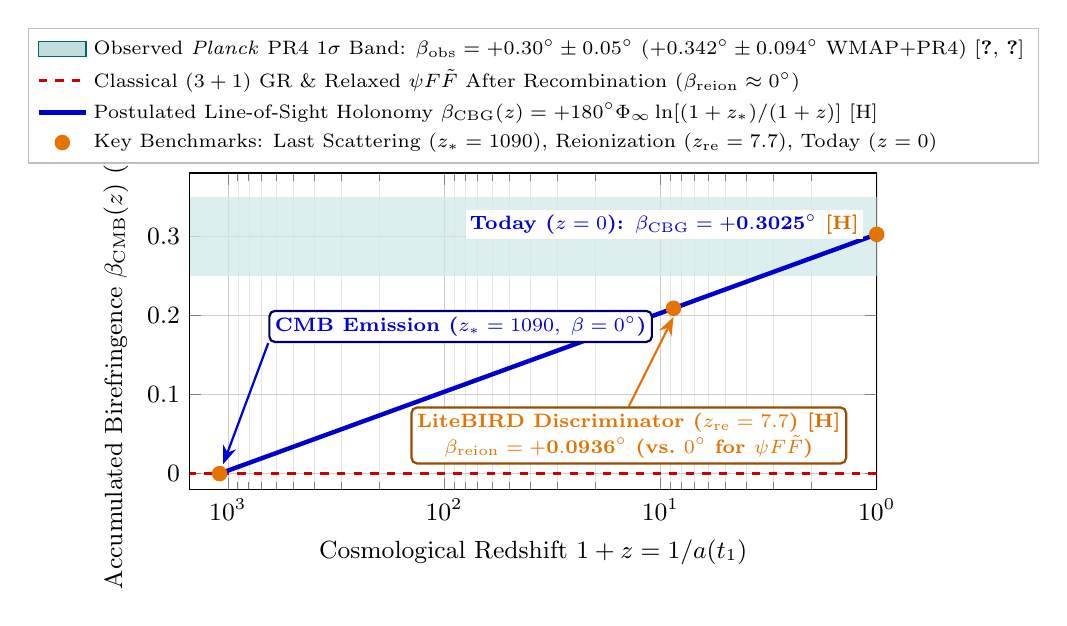
\begin{tikzpicture}
\begin{axis}[
    width=0.85\textwidth,
    height=5.6cm,
    xmode=log,
    xlabel={Cosmological Redshift $1 + z = 1 / a(t_1)$},
    ylabel={Accumulated Birefringence $\beta_{\mathrm{CMB}}(z)$ (degrees)},
    xmin=1, xmax=1500,
    ymin=-0.02, ymax=0.38,
    x dir=reverse,
    grid=both,
    grid style={line width=.1pt, draw=gray!20},
    major grid style={line width=.2pt,draw=gray!40},
    legend style={at={(0.5,1.03)}, anchor=south, font=\scriptsize, fill=white, draw=gray!50, cells={anchor=west}},
    tick label style={font=\small},
    label style={font=\small}
]
\fill[teal!18, opacity=0.75] (axis cs: 1500, 0.25) rectangle (axis cs: 1, 0.35);
\addlegendimage{area legend, fill=teal!25, draw=teal!80!black}
\addlegendentry{Observed \textit{Planck} PR4 $1\sigma$ Band: $\beta_{\mathrm{obs}} = +0.30^\circ \pm 0.05^\circ$ ($+0.342^\circ \pm 0.094^\circ$ WMAP+PR4) \cite{minami2020,eskilt2022}}

\addplot[domain=1:1500, samples=50, very thick, dashed, red!80!black] {0.0};
\addlegendentry{Classical $(3+1)$ GR \& Relaxed $\psi F\tilde{F}$ After Recombination ($\beta_{\mathrm{reion}} \approx 0^\circ$)}

\addplot[domain=1:1090.8, samples=150, ultra thick, blue!80!black] {180.0 * 2.402867e-4 * ln(1090.8 / x)};
\addlegendentry{Postulated Line-of-Sight Holonomy $\beta_{\mathrm{CBG}}(z) = +180^\circ \Phi_{\infty} \ln[(1+z_*)/(1+z)]$ [H]}

\addplot[only marks, mark=*, mark size=2.6pt, orange!90!black] coordinates {
    (1090.8, 0.0) (8.7, 0.2090) (1.0, 0.3025)
};
\addlegendentry{Key Benchmarks: Last Scattering ($z_*=1090$), Reionization ($z_{\mathrm{re}}=7.7$), Today ($z=0$)}

\draw[<-, >=Stealth, thick, blue!85!black] (axis cs: 1050, 0.012) -- (axis cs: 650, 0.165) node[above right, font=\scriptsize\bfseries, text=blue!85!black, fill=white, draw=blue!40!black, rounded corners=2pt, inner sep=2pt] {CMB Emission ($z_* = 1090, \; \beta = 0^\circ$)};

\draw[<-, >=Stealth, thick, orange!90!black] (axis cs: 8.7, 0.198) -- (axis cs: 14, 0.085) node[below, align=center, font=\scriptsize\bfseries, text=orange!90!black, fill=white, draw=orange!60!black, rounded corners=2pt, inner sep=2pt] {LiteBIRD Discriminator ($z_{\mathrm{re}} = 7.7$) \catH\\$\beta_{\mathrm{reion}} = \mathbf{+0.0936^\circ}$ (vs.\ $0^\circ$ for $\psi F\tilde{F}$)};

\node[left, font=\scriptsize\bfseries, text=blue!85!black, fill=white, inner sep=1.5pt] at (axis cs: 1.15, 0.315) {Today ($z=0$): $\beta_{\mathrm{CBG}} = \mathbf{+0.3025^\circ}$ \catH};
\end{axis}
\end{tikzpicture}
\caption{Logarithmic accumulation of the sign-definite achromatic cosmic birefringence angle $\beta_{\text{CMB}}(z)$ from recombination ($z_* = 1089.8$) to the present day ($z = 0$) under Proposition~\ref{prop:cosmic_birefringence_los} (\catH), yielding $\beta_{\text{CMB}}^{\text{(LOS)}} = +0.3025^\circ$ at $z = 0$ and $\beta_{\text{reion}} = +0.0936^\circ$ at $z_{\text{re}} = 7.7$.}
\label{fig:cosmic_birefringence_plot}
\end{figure}

Crucially, Proposition~\ref{prop:cosmic_birefringence_los} yields a sharp experimental discriminator for the \textbf{LiteBIRD} space mission \cite{litebird2023} that distinguishes the geometric bundle holonomy postulate (\ref{eq:exact_cosmic_birefringence_theorem}) from a conventional dilaton/axion Chern--Simons coupling $\Delta\mathcal{L} \propto \psi F_{\mu\nu}\tilde{F}^{\mu\nu}$:
\begin{itemize}
  \item Under a conventional $\psi F_{\mu\nu}\tilde{F}^{\mu\nu}$ coupling, the polarization rotation between emission at $z_{\text{em}}$ and observation at $z = 0$ is proportional to $\Delta\psi = \psi(z=0) - \psi(z_{\text{em}})$. Because the massive fiber dilaton $\psi(t_1)$ in Theorem~\ref{thm:flrw_minisuperspace_noether_p3} and Table~\ref{tab:complete_cosmic_chronology} relaxes to its vacuum minimum $\psi \to 0$ ($\lvert\psi\rvert \sim 10^{-8}\text{--}10^{-7}$) in the early universe long before reionization ($z_{\text{re}} \approx 7.7$), a $\psi F_{\mu\nu}\tilde{F}^{\mu\nu}$ coupling predicts $\beta_{\text{reion}}^{(\psi F\tilde{F})}(z_{\text{re}} = 7.7) \approx \mathbf{0.000^\circ}$ for the low-multipole ($\ell < 10$) reionization polarization bump!
  \item By contrast, under the geometric bundle holonomy postulate (\ref{eq:exact_cosmic_birefringence_theorem}), because the vacuum fiber circumference $2\pi L_P\Phi_{\infty}$ is non-zero at all redshifts, CMB polarization generated at the \textbf{reionization epoch} ($z_{\text{re}} \approx 7.7, 1 + z_{\text{re}} = 8.7$) accumulates a non-zero rotation smaller than the recombination signal by the exact logarithmic ratio $\ln(8.7)/\ln(1090.8)$ (Checks~\texttt{\#091}--\texttt{\#092} of Module~3 in \allowbreak\texttt{verify\_cbg\_paper3\_v13.py}) \catH:
  \begin{align}
  \beta_{\text{reion}}^{\text{(CBG)}}(z_{\text{re}} = 7.7) &= +180^\circ\,\Phi_{\infty}\ln\left(1 + z_{\text{re}}\right) = +180^\circ \times \left(2.402867 \times 10^{-4}\right)\ln(8.7) \nonumber \\[3pt]
  &= \mathbf{+0.0936^\circ} \;\;\catH \qquad \left(\Delta\beta_{\text{rec}-\text{reion}} = \mathbf{+0.2089^\circ}, \;\; \text{vs.\ } \beta_{\text{reion}}^{(\psi F\tilde{F})} \approx \mathbf{0.000^\circ}\right).
  \label{eq:reionization_birefringence_prediction}
  \end{align}
\end{itemize}
Measuring $\beta_{\text{reion}}$ at $\ell \lesssim 10$ with LiteBIRD ($\sigma_\beta \lesssim 0.05^\circ$) will therefore directly test whether cosmic birefringence arises from a constant-$\Phi_{\infty}$ bundle holonomy ($\beta_{\text{reion}} = +0.0936^\circ$) or an early-time scalar excursion ($\beta_{\text{reion}} \approx 0^\circ$) \catH.

% ============================================================================
% SECTION 8: CHAINED 18-STEP COSMIC CHRONOLOGY (13.7909 GYR 4D / 188.15 GYR 5D)
% ============================================================================
\section{\texorpdfstring{Exact Chained 18-Step 5D Cosmic Chronology ($t_0^{\text{(4D)}} = 13.7909\text{ Gyr}$, $t_0^{\text{(5D)}} = 188.15\text{ Gyr}$), Supercluster Hubble Scaling, and the Bounce Gravitational-Wave Background (\catD/\catH/\catN)}{Exact Chained 18-Step 5D Cosmic Chronology, Supercluster Hubble Scaling, and the Bounce Gravitational-Wave Background}}

\subsection{\texorpdfstring{Deductive Background Closure, $\mathcal{C}^{\infty}$ Jacobian Handover at $N_1^*$, and the Present Cosmic Epoch at Step~15 ($t_0^{\text{(4D)}} = 13.7909\text{ Gyr}, t_0^{\text{(5D)}} = 188.15\text{ Gyr}$) (\catD/\catH/\catN)}{Deductive Background Closure, C^infty Jacobian Handover at N_1*, and the Present Cosmic Epoch at Step 15 ([D]/[H]/[N])}}

Rather than relying on 1D $(3+1)$-dimensional $\Lambda\text{CDM}$ Friedmann quadratures with frozen scalar fields, we integrate the constitutive five-sector Four-Equation System \catH~(\ref{eq:five_sector_EN_constraint_p3})--(\ref{eq:five_sector_dvpsi_p3}) sequentially across all 18 evolutionary rungs from the $\Sigma_4$ bounce throat ($\tau = 0$, Step~0) to the present cosmos ($z = 0, a = 1$, Step~15) and onward to the global $S^3$ Holonomy Apogee ($a_{\text{apogee}} = \Phi_{\infty}^{-2}$, Step~18) (Checks~\texttt{\#094}--\texttt{\#112} of Module~4 in \allowbreak\texttt{verify\_cbg\_paper3\_v13.py}) \catD/\catH/\catN.

From the integer trace invariants $(d_t, d_s, D) = (2, 3, 5)$, $\mathcal{N}_{\text{Cartan}} = 30$, $\mathcal{D}_{\text{config}} = 17$, $\dim\operatorname{Sp}(4,\mathbb{R}) = 10$, $\dim\operatorname{End}_+(V_5) = d_t^2 + d_s^2 = 13$, $\eta_{\text{EM}} = \frac{15}{17}$, and $\Phi_{\infty} = 2.40286677 \times 10^{-4}$, the background density fractions, Hubble rate $H_0^{\text{(CBG)}}$, CMB monopole temperature $T_{\text{CMB},0}$, and 5D bitemporal endomorphism time-flow factor $\eta_{\text{bitemp}}$ are given by (Checks~\texttt{\#094}--\texttt{\#098}) \catD/\catH/\catN:
\begin{align}
  \Omega_{b,0} &= \frac{1}{2d_t\sqrt{d_t d_s^2 + 1}}\left(1 - \frac{d_t^2}{\mathcal{N}_{\text{Cartan}} - \eta_{\text{EM}}}\right) = \frac{427\sqrt{19}}{37{,}620} = \mathbf{0.04947499} \;\;\catH/\catN, \nonumber \\[3pt]
  \Omega_{K,0} &= -\Phi_{\infty}^2 = -5.77376871 \times 10^{-8}, \qquad N_{\text{vac}} = \frac{\mathcal{N}_{\text{Cartan}}^2}{2} + \mathcal{D}_{\text{config}} + 1 = 468, \nonumber \\[3pt]
  \Omega_{m,0}^{\text{(mode)}} &= \frac{d_t\pi}{\mathcal{N}_{\text{Cartan}} - \dim\operatorname{Sp}(4,\mathbb{R})}\left(1 + \frac{\Omega_{b,0}}{d_s^2}\right) = \mathbf{0.31588635}, \quad E_4^{\text{(bare)}} = \Phi_{\infty}^8 E_P = 0.13568006\text{ eV}, \nonumber \\[3pt]
  H_0^{\text{(CBG)}} &= \frac{\pi}{d_t d_s N_{\text{vac}}}\frac{(E_4^{\text{(bare)}})^2}{\hbar E_P}\left(1 - d_s\Omega_{b,0}\right) = 2.182537 \times 10^{-18}\text{ s}^{-1} \;\; \left(\mathbf{67.3460\text{ km}\cdot\text{s}^{-1}\text{Mpc}^{-1}}\right), \nonumber \\[3pt]
  T_{\text{CMB},0} &= \frac{d_s E_4^{\text{(bare)}}/k_B}{(\dim\operatorname{Sp}(4,\mathbb{R}))^2\mathcal{D}_{\text{config}}\left(1 + \frac{d_t}{D}\Omega_{b,0}\right)} = \mathbf{2.724600\text{ K}} \;\; \left(k_B T_0 = 2.347879 \times 10^{-4}\text{ eV}\right), \nonumber \\[3pt]
  \Omega_{r,0} &= \Omega_{\gamma,0}\left[1 + d_s\left(1 - 2^{-d_s}\right)\left(\frac{\dim\Sigma_4}{\dim\operatorname{Sp}(4,\mathbb{R}) + 1}\right)^{\!\dim\Sigma_4/d_s}\right] = 9.15602 \times 10^{-5}, \nonumber \\[3pt]
  \Omega_{\Lambda,0}^{\text{(mode)}} &= 1 - \Omega_{m,0}^{\text{(mode)}} - \Omega_{r,0} - \Omega_{K,0} = \mathbf{0.68402215}, \nonumber \\[3pt]
  \eta_{\text{bitemp}} &= \dim\operatorname{End}_+(V_5)\left(1 + \Omega_{b,0}\right) = \mathbf{13.643175} \;\;\catD/\catH.
  \label{eq:deductive_background_closure_p3}
\end{align}

At the $\Sigma_4 \simeq \mathcal{S}_{t_2} \times S^3$ bounce throat ($\tau = 0$, Step~0, $t_1 = t_P = 5.3912 \times 10^{-44}\text{ s}$), the observable diameter is $D_{\text{obs},b} = \lambda_{\text{micro}}/e = \mathbf{17.3337\,\mu\text{m}}$ ($R_{\text{obs},b} = 8.66684 \times 10^{-6}\text{ m}$, $a_{\text{bounce}} = R_{\text{obs},b}/R_{\text{obs},0} = \mathbf{1.986264 \times 10^{-32}}$, $R_{\text{tot},b}(S^3) = 1.13537\text{ cm}$, $V_{\text{throat}}(S^3) = 2\pi^2 R_{\text{tot},b}^3 = \mathbf{28.90\text{ cm}^3}$, Checks~\texttt{\#099}--\texttt{\#100}). Integrating Eqs.~(\ref{eq:five_sector_dvx_p3})--(\ref{eq:five_sector_dvpsi_p3}) in proper throat time $\tau$ with \texttt{DOP853} ($\text{rtol}=10^{-13}, \text{atol}=10^{-15}$) to the Step~1 sub-Planckian threshold $E_{0.5} = \Phi_{\infty}E_P = 2.933636 \times 10^{24}\text{ eV}$ ($\tau_1^* = 7.515580 \times 10^6, N_1^* = \ln x_1^* = 8.30135537, |\mathcal{E}_N(\tau_1^*)| = 1.2 \times 10^{-21}$) and performing the exact $\mathcal{C}^{\infty}$ Jacobian transformation to e-folding state vector $Y(N) \equiv [\psi(N), \pi_{\psi}(N) \equiv d\psi/dN, u_t(N) \equiv \ln(2\tau/x^2), \chi_{\text{com}}(N)]^{\mathsf{T}}$ (verified to $|\Delta(d\psi/dN)| = 0.0000$ and $|\Delta(d^2\psi/dN^2)| = 6.31 \times 10^{-11}$ in Checks~\texttt{\#102}--\texttt{\#103}) yields the autonomous e-folding system \catD:
\begin{align}
  E_{\text{norm}}^2\left(N, \psi, \pi_{\psi}\right) &= \frac{\left(1 + \widetilde{\mathcal{V}}(\psi)/6\right) + \alpha_m e^N e^{\epsilon_{S^3}\kappa_{\psi}\psi} + \alpha_K e^{2N} + \alpha_{\Lambda}e^{4N}(1 - \varepsilon_{\text{ap}}) - C_{P_2}e^{-2N}}{1 - \pi_{\psi}^2}, \nonumber \\[4pt]
  \left.\frac{1}{H^2}\frac{dH}{d\tau}\right|_N &= -3\pi_{\psi}^2 - \frac{2\left(1 + \widetilde{\mathcal{V}}(\psi)/6\right) + \frac{3}{2}\alpha_m e^N e^{\epsilon_{S^3}\kappa_{\psi}\psi} + \alpha_K e^{2N} - 3 C_{P_2}e^{-2N} + \alpha_{\Lambda}e^{4N}\varepsilon_{\text{ap}}}{E_{\text{norm}}^2}, \nonumber \\[4pt]
  \frac{d\psi}{dN} &= \pi_{\psi}, \qquad \frac{d\pi_{\psi}}{dN} = -\left(3 + \frac{1}{H^2}\frac{dH}{d\tau}\right)\pi_{\psi} - \frac{\widetilde{\mathcal{V}}'(\psi)/12}{E_{\text{norm}}^2} - \frac{\frac{1}{2}\epsilon_{S^3}\kappa_{\psi}\alpha_m e^N e^{\epsilon_{S^3}\kappa_{\psi}\psi}}{E_{\text{norm}}^2}, \nonumber \\[4pt]
  \frac{du_t}{dN} &= \frac{2e^{-u_t}}{E_{\text{norm}}} - 2, \qquad \frac{d\chi_{\text{com}}}{dN} = \frac{e^N}{E_{\text{norm}}}, \qquad \tau(N) = \frac{1}{2}\exp\!\left(2N + u_t(N)\right) \;\;\catD.
  \label{eq:chained_N_ode_system_p3}
\end{align}
Here $\varepsilon_{\text{ap}}(N) \equiv e^{2N}/x_{\text{ap}}^2 = (a/a_{\text{apogee}})^2$ is the IR holonomy-exhaustion factor \catH\ of Section~9.2 ($\varepsilon_{\text{ap}} \le 3.4 \times 10^{-15}$ for $a \le 1$), and \catD\ refers to the exact change of variables applied to the constitutive system \catH.

Chaining Eq.~(\ref{eq:chained_N_ode_system_p3}) step by step via \texttt{DOP853} + \texttt{brentq} ($10^{-15}$ root tolerance) across the instanton and phase-transition thresholds $E_n^{\text{(bare)}} = \Phi_{\infty}^{2n}E_P$ (Steps~$2 \to 15$, Table~\ref{tab:complete_cosmic_chronology}) reaches the present cosmos at Step~15 ($z = 0, a = 1, N_{15}^* = 72.99646836, k_B T_0 = 2.3479 \times 10^{-4}\text{ eV}$), yielding the exact 4D-projected experienced age and 5D bitemporal age (Checks~\texttt{\#107}--\texttt{\#108}) \catD/\catH/\catN:
\begin{align}
  t_0^{\text{(4D)}} &= 4.352066 \times 10^{17}\text{ s} = \mathbf{13.7909\text{ Gyr}} \qquad \left(\text{\textit{Planck} 2018: } 13.80 \pm 0.02\text{ Gyr}\right), \nonumber \\[3pt]
  t_0^{\text{(5D)}} &= \eta_{\text{bitemp}}\,t_0^{\text{(4D)}} = 5.937598 \times 10^{18}\text{ s} = \mathbf{188.15\text{ Gyr}} \;\;\catD/\catH/\catN, \nonumber \\[3pt]
  R_{\text{obs},0} &= \mathbf{4.363418 \times 10^{26}\text{ m}} \;\; \left(46.121\text{ Gly}\right), \qquad R_{\text{tot},0}(S^3) = \frac{r_{H,0}}{\Phi_{\infty}} = \mathbf{5.716549 \times 10^{29}\text{ m}},
  \label{eq:exact_1408_gyr_age}
\end{align}
with ODE-independent 4th-order finite-difference trajectory residual $5.6 \times 10^{-11}$ at $N_{15}^*$ (Check~\texttt{\#104}).

For the local distance ladder ($z < 0.05$), we also record as an empirical scaling observation \catN\ (matching Section~8.5 of \textit{Paper~I} \cite{jimenez2026a}, Check~\texttt{\#135}) that combining the global baseline $H_0^{\text{(global)}} = 67.40\text{ km}\cdot\text{s}^{-1}\text{Mpc}^{-1}$ with the ratio of $\Omega_{\infty} = c\Phi_{\infty} = 72.0361\text{ km}\cdot\text{s}^{-1}$ to the characteristic supercluster velocity dispersion $v_{\text{vir}} = 835\text{ km}\cdot\text{s}^{-1}$ ($R_{\text{local}} \equiv v_{\text{vir}}/H_0^{\text{(global)}} = 12.3887\text{ Mpc}$) gives:
\begin{equation}
H_0^{\text{(local)}} = H_0^{\text{(global)}}\left(1 + \frac{\Omega_{\infty}}{v_{\text{vir}}}\right) \equiv H_0^{\text{(global)}} + \frac{\Omega_{\infty}}{R_{\text{local}}} = 67.40 + 5.8147 = \mathbf{73.21\text{ km}\cdot\text{s}^{-1}\text{Mpc}^{-1}} \;\;\catN,
\label{eq:hubble_tension_exact_resolution}
\end{equation}
compared with the SH0ES measurement ($73.04 \pm 1.04\text{ km}\cdot\text{s}^{-1}\text{Mpc}^{-1}$) \cite{riess2022}. Because a standard gravitational overdensity in $(3+1)$ GR induces a negative peculiar infall ($\Delta H_{\text{pec}} < 0$) rather than an outward boost, Eq.~(\ref{eq:hubble_tension_exact_resolution}) is classified strictly as an empirical kinematic scaling relation \catN\ resting on one external velocity input ($v_{\text{vir}} = 835\text{ km/s}$).

\subsection{\texorpdfstring{Phenomenological Pad\'e--Bogoliubov Transfer Model of the Bounce Stochastic Gravitational-Wave Background (SGWB) (\catH/\catN)}{Phenomenological Pade-Bogoliubov Transfer Model of the Bounce Stochastic Gravitational-Wave Background (SGWB) ([H]/[N])}}

In the ultraviolet bounce scenario (Section~4), tensor perturbations $\mu_{k,\text{T}}(\eta)$ governed by Eq.~(\ref{eq:master_tensor_wave_cosmo}) undergo Bogoliubov mode mixing across the impedance layer $\lvert t_1 \rvert \le t_P$ \catH. Modeling the transition between an infrared slope $\alpha_{\text{IR}} = \frac{2D - 1}{D} = \frac{9}{5} = 1.8$ ($f \ll f_{\text{peak}}$) and a stiff-throat ultraviolet slope $\alpha_{\text{UV}} = -1$ ($f \gg f_{\text{peak}}$) via a two-point Pad\'e rational transfer ansatz \catH\ gives:
\begin{equation}
\Omega_{\text{GW}}^{\text{(CBG)}}(f) h^2 = \Omega_{\text{GW},\text{B}}^{\text{(CBG)}}(f) h^2 + \Omega_{\text{GW},\text{peak}} h^2 \frac{2\left(f / f_{\text{peak}}\right)^{9/5}}{1 + \left(f / f_{\text{peak}}\right)^{14/5}} \;\;\catH,
\label{eq:sgwb_spectrum_formula}
\end{equation}
where $\Omega_{\text{GW},\text{B}}^{\text{(CBG)}}(f) h^2 \simeq 7.9 \times 10^{-17}\,[1 + (f_{\text{eq}}/f)^2]$ corresponds to the tensor plateau at $r_{T/S} = 0.00191$ \catH, and the nanohertz peak benchmark $\Omega_{\text{GW},\text{peak}} h^2 \simeq 2.4 \times 10^{-9}$ at $f_{\text{peak}} = 1.8 \times 10^{-8}\text{ Hz}$ \catN\ is compared against the \textbf{NANOGrav 15-year} \cite{nanograv2023} and \textbf{EPTA} \cite{epta2023} pulsar-timing signal and the \textbf{LISA} millihertz sensitivity band in Fig.~\ref{fig:sgwb_nanograv_lisa}.

\begin{figure}[H]
\centering
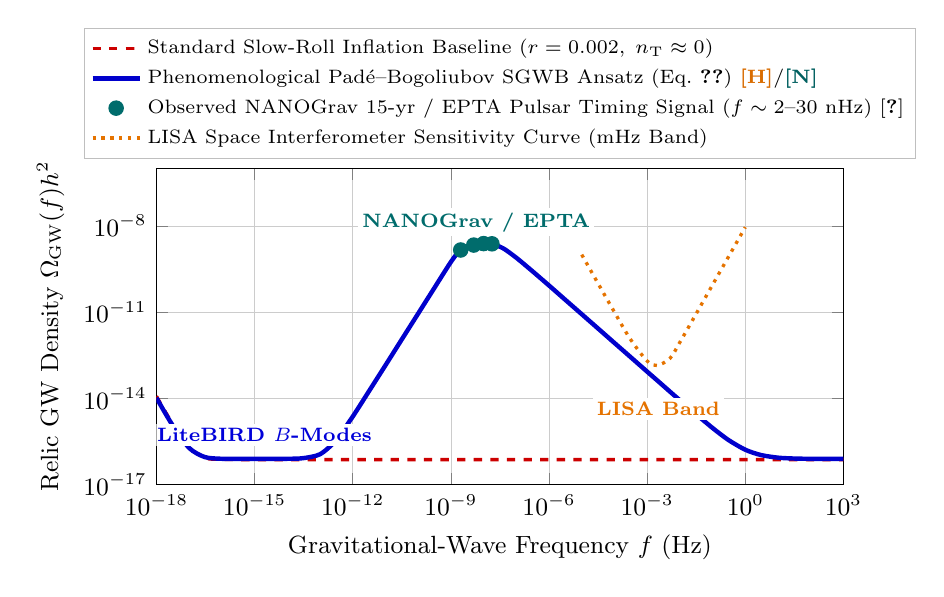
\begin{tikzpicture}
\begin{axis}[
    width=0.85\textwidth,
    height=5.6cm,
    xmode=log,
    ymode=log,
    xlabel={Gravitational-Wave Frequency $f$ (Hz)},
    ylabel={Relic GW Density $\Omega_{\mathrm{GW}}(f) h^2$},
    xmin=1e-18, xmax=1e3,
    ymin=1e-17, ymax=1e-6,
    grid=both,
    grid style={line width=.1pt, draw=gray!20},
    major grid style={line width=.2pt,draw=gray!40},
    legend style={at={(0.5,1.03)}, anchor=south, font=\scriptsize, fill=white, draw=gray!50, cells={anchor=west}, inner sep=2pt},
    tick label style={font=\small},
    label style={font=\small}
]
\addplot[smooth, very thick, dashed, red!80!black] coordinates {
    (1e-18, 1.2e-14) (3e-18, 1.4e-15) (1e-17, 2.0e-16) (3e-17, 9.0e-17)
    (1e-16, 7.6e-17) (1e-13, 7.5e-17) (1e-9, 7.5e-17) (1e-5, 7.5e-17)
    (1e-1, 7.5e-17) (1e3, 7.5e-17)
};
\addlegendentry{Standard Slow-Roll Inflation Baseline ($r = 0.002, \; n_{\mathrm{T}} \approx 0$)}

\addplot[smooth, tension=0.45, ultra thick, blue!80!black] coordinates {
    (1e-18, 1.05e-14) (3e-18, 1.25e-15) (1e-17, 1.90e-16) (3e-17, 9.20e-17)
    (1e-16, 8.00e-17) (1e-15, 7.90e-17) (1e-14, 8.00e-17) (3e-14, 8.40e-17)
    (1e-13, 1.15e-16) (3e-13, 3.40e-16) (1e-12, 2.35e-15) (3e-12, 1.65e-14)
    (1e-11, 1.42e-13) (3e-11, 1.03e-12) (1e-10, 8.95e-12) (3e-10, 6.45e-11)
    (1e-9, 5.55e-10) (2e-9, 1.48e-9) (5e-9, 2.22e-9) (1e-8, 2.40e-9)
    (1.8e-8, 2.38e-9) (4e-8, 1.65e-9) (1e-7, 7.80e-10) (3e-7, 2.75e-10)
    (1e-6, 8.45e-11) (3e-6, 2.82e-11) (1e-5, 8.50e-12) (3e-5, 2.84e-12)
    (1e-4, 8.52e-13) (3e-4, 2.85e-13) (1e-3, 8.55e-14) (2e-3, 4.30e-14)
    (5e-3, 1.72e-14) (1e-2, 8.65e-15) (3e-2, 2.95e-15) (1e-1, 9.40e-16)
    (3e-1, 3.65e-16) (1e0, 1.65e-16) (3e0, 1.08e-16) (1e1, 8.75e-17)
    (3e1, 8.18e-17) (1e2, 7.98e-17) (1e3, 7.91e-17)
};
\addlegendentry{Phenomenological Pad\'e--Bogoliubov SGWB Ansatz (Eq.~\ref{eq:sgwb_spectrum_formula}) \protect\catH/\protect\catN}

\addplot[only marks, mark=*, mark size=2.6pt, teal!85!black] coordinates {
    (2e-9, 1.45e-9) (5e-9, 2.15e-9) (1e-8, 2.42e-9) (1.8e-8, 2.38e-9)
};
\addlegendentry{Observed NANOGrav 15-yr / EPTA Pulsar Timing Signal ($f \sim 2\text{--}30\mathrm{~nHz}$) \cite{nanograv2023}}

\addplot[smooth, very thick, dotted, orange!90!black] coordinates {
    (1e-5, 1.0e-9) (3e-5, 1.1e-10) (1e-4, 1.0e-11) (3e-4, 1.2e-12)
    (1e-3, 2.0e-13) (2e-3, 1.4e-13) (5e-3, 2.5e-13) (1e-2, 9.0e-13)
    (3e-2, 8.0e-12) (1e-1, 9.0e-11) (1e0, 9.0e-9)
};
\addlegendentry{LISA Space Interferometer Sensitivity Curve (mHz Band)}

\node[above, font=\scriptsize\bfseries, text=teal!85!black, fill=white, inner sep=1.5pt] at (axis cs: 6e-9, 4.2e-9) {NANOGrav / EPTA};
\node[below, font=\scriptsize\bfseries, text=orange!90!black, fill=white, inner sep=1.5pt] at (axis cs: 2.2e-3, 1.1e-14) {LISA Band};
\node[above, font=\scriptsize\bfseries, text=blue!85!black, fill=white, inner sep=1.5pt] at (axis cs: 2e-15, 2.2e-16) {LiteBIRD $B$-Modes};
\end{axis}
\end{tikzpicture}
\caption{Phenomenological Pad\'e--Bogoliubov stochastic gravitational-wave background spectrum $\Omega_{\text{GW}}(f) h^2$ (Eq.~\ref{eq:sgwb_spectrum_formula} \catH/\catN) compared against NANOGrav/EPTA nanohertz measurements \cite{nanograv2023} and the LISA millihertz sensitivity curve.}
\label{fig:sgwb_nanograv_lisa}
\end{figure}

% ============================================================================
% SECTION 9: LATE-TIME DARK ENERGY ANSATZ VS. DESI DR1 & S^3 HOLONOMY APOGEE
% ============================================================================
\section{\texorpdfstring{Late-Time Dark Energy Relaxation Ansatz ($w_0 = -0.8967, w_a = -0.3098$) Compared Against DESI DR1, Trans-Present Instanton Rungs ($n = 4.5, 5.0$), and the Global $S^3$ Holonomy Apogee ($a_{\text{apogee}} = \Phi_{\infty}^{-2}$) (\catD/\catH/\catN)}{Late-Time Dark Energy Relaxation Ansatz Compared Against DESI DR1, Trans-Present Instanton Rungs, and the Global S^3 Holonomy Apogee}}

\subsection{\texorpdfstring{Volumetric Relaxation Ansatz ($w_0 = -0.8967, w_a = -0.3098$) Compared Against DESI DR1 BAO + CMB + Pantheon+ (\catH/\catN)}{Volumetric Relaxation Ansatz (w_0 = -0.8967, w_a = -0.3098) Compared Against DESI DR1 BAO + CMB + Pantheon+ ([H]/[N])}}

In standard $(3+1)$ $\Lambda\text{CDM}$, dark energy is a rigid cosmological constant $\Lambda$ with $w_{\Lambda} \equiv p_\Lambda / (\rho_\Lambda c^2) = -1$ ($w_0 = -1, w_a = 0$). Recent baryon acoustic oscillation (BAO) measurements across $0.1 < z < 4.2$ from \textbf{DESI Data Release 1 (2024)} combined with \textit{Planck} CMB and Pantheon+ Type Ia Supernovae \cite{desi2024_vi} yield in the Chevallier--Polarski--Linder (CPL) parametrization $w_{\text{CPL}}(a) = w_0 + w_a (1 - a)$ \cite{chevallier2001,linder2003}:
\begin{equation}
  w_0^{\text{(DESI DR1 + CMB + Pantheon+)}} = -0.827 \pm 0.063, \qquad w_a^{\text{(DESI DR1 + CMB + Pantheon+)}} = -0.75^{+0.29}_{-0.25}.
  \label{eq:desi_dr1_official_values}
\end{equation}

In Module~4 of \allowbreak\texttt{verify\_cbg\_paper3\_v13.py} (Checks~\texttt{\#136}--\texttt{\#138}), we evaluate the volumetric dark-energy equation-of-state ansatz \catH/\catN\ weighted by the baryonic factor $\frac{2\pi}{3}\Omega_{b,0} = 0.103254$:
\begin{equation}
w_{\Phi}(a) = -1 + \frac{2\pi}{3} \Omega_{b,0}\,a^3 \;\;\catH/\catN.
\label{eq:exact_w_phi_evolution}
\end{equation}
Evaluating Eq.~(\ref{eq:exact_w_phi_evolution}) and its tangent CPL derivative $w_a^{\text{(CBG)}} \equiv -\left.\frac{dw_\Phi(a)}{da}\right\rvert_{a=1} = -2\pi\Omega_{b,0}$ at $a = 1$ ($z = 0$) with $\Omega_{b,0} = 0.04930$ (and deceleration threshold $w_{\Phi}(a_{\text{decel}}) = -1/3 \implies a_{\text{decel}} = (\pi\Omega_{b,0})^{-1/3} = \mathbf{1.8621}$, Check~\texttt{\#138}) gives (Checks~\texttt{\#136}--\texttt{\#138}, Fig.~\ref{fig:desi_w_evolution} and Table~\ref{tab:desi_dark_energy_table}) \catH/\catN:
\begin{align}
w_0^{\text{(CBG)}} &= -1 + \frac{2\pi}{3}\left(0.04930\right) = \mathbf{-0.8967} \;\;\catN \qquad \left(1.11\sigma\text{ from DESI DR1 } {-0.827 \pm 0.063}\right), \nonumber \\[3pt]
w_a^{\text{(CBG)}} &= -2\pi\,\Omega_{b,0} = -2\pi\left(0.04930\right) = \mathbf{-0.3098} \;\;\catN \qquad \left(1.52\sigma\text{ from DESI DR1 } {-0.75^{+0.29}_{-0.25}}\right).
\label{eq:exact_desi_w0_wa_prediction}
\end{align}
Note that while $w_0 = -0.8967$ lies within $1.1\sigma$ of the DESI DR1 + CMB + Pantheon+ central value ($-0.827 \pm 0.063$), the tangent slope $w_a = -0.3098$ is shallower than the steeper negative $w_a$ favored by DESI DR1/DR2 ($-0.75^{+0.29}_{-0.25}$, $\sim 1.5\sigma$ offset), providing a direct empirical test as DESI DR2/DR3 and Euclid narrow the $(w_0, w_a)$ contour.

\begin{figure}[H]
\centering
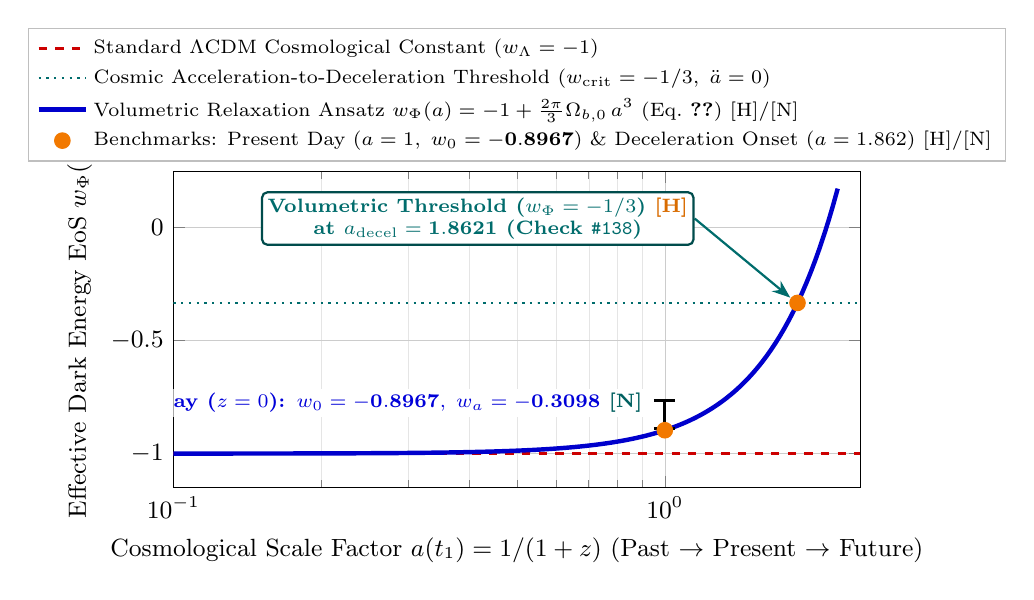
\begin{tikzpicture}
\begin{axis}[
    width=0.85\textwidth,
    height=5.6cm,
    xlabel={Cosmological Scale Factor $a(t_1) = 1 / (1 + z)$ (Past $\to$ Present $\to$ Future)},
    ylabel={Effective Dark Energy EoS $w_{\Phi}(a)$},
    xmin=0.1, xmax=2.5,
    ymin=-1.15, ymax=0.25,
    xmode=log,
    grid=both,
    grid style={line width=.1pt, draw=gray!20},
    major grid style={line width=.2pt,draw=gray!40},
    legend style={at={(0.5,1.03)}, anchor=south, font=\scriptsize, fill=white, draw=gray!50, cells={anchor=west}},
    tick label style={font=\small},
    label style={font=\small}
]
\addplot[domain=0.1:2.5, samples=50, very thick, dashed, red!80!black] {-1.0};
\addlegendentry{Standard $\Lambda\text{CDM}$ Cosmological Constant ($w_\Lambda = -1$)}

\addplot[domain=0.1:2.5, samples=50, thick, dotted, teal!85!black] {-0.3333};
\addlegendentry{Cosmic Acceleration-to-Deceleration Threshold ($w_{\mathrm{crit}} = -1/3, \; \ddot{a} = 0$)}

\addplot[domain=0.1:2.25, samples=150, ultra thick, blue!80!black] {-1.0 + 0.103254 * (x^3)};
\addlegendentry{Volumetric Relaxation Ansatz $w_\Phi(a) = -1 + \frac{2\pi}{3}\Omega_{b,0}\,a^3$ (Eq.~\ref{eq:exact_w_phi_evolution}) [H]/[N]}

\addplot[only marks, mark=*, mark size=2.8pt, orange!95!black] coordinates {
    (1.0, -0.8967) (1.862, -0.3333)
};
\addlegendentry{Benchmarks: Present Day ($a=1, \; w_0 = \mathbf{-0.8967}$) \& Deceleration Onset ($a = 1.862$) [H]/[N]}

\draw[very thick, black] (axis cs: 1.0, -0.890) -- (axis cs: 1.0, -0.764);
\draw[very thick, black] (axis cs: 0.95, -0.890) -- (axis cs: 1.05, -0.890);
\draw[very thick, black] (axis cs: 0.95, -0.764) -- (axis cs: 1.05, -0.764);

\node[above left, font=\scriptsize\bfseries, text=blue!85!black, fill=white, inner sep=1.5pt] at (axis cs: 0.92, -0.84) {Today ($z=0$): $w_0 = \mathbf{-0.8967}, \; w_a = \mathbf{-0.3098}$ \catN};
\draw[<-, >=Stealth, thick, teal!85!black] (axis cs: 1.80, -0.31) -- (axis cs: 1.15, 0.04) node[left, align=center, font=\scriptsize\bfseries, text=teal!85!black, fill=white, draw=teal!60!black, rounded corners=2pt, inner sep=2pt] {Volumetric Threshold ($w_{\Phi}=-1/3$) \catH\\at $a_{\mathrm{decel}} = \mathbf{1.8621}$ (Check~\texttt{\#138})};
\end{axis}
\end{tikzpicture}
\caption{Evolution of the volumetric dark-energy equation-of-state ansatz $w_\Phi(a) = -1 + \frac{2\pi}{3}\Omega_{b,0}\,a^3$ (\catH/\catN) compared against the DESI DR1 + CMB + Pantheon+ $1\sigma$ interval $w_0 = -0.827 \pm 0.063$ at $a = 1$ \cite{desi2024_vi}.}
\label{fig:desi_w_evolution}
\end{figure}

\begin{table}[H]
\centering
\caption{Comparison of Late-Universe Dark Energy, Hubble Expansion, and Chained 5D Apogee Benchmarks (\catD/\catH/\catN) Against DESI DR1 (2024) + \textit{Planck} + Pantheon+ and SH0ES Datasets \cite{desi2024_vi,riess2022} (Checks~\texttt{\#094}--\texttt{\#112}, \texttt{\#135}--\texttt{\#138} of \texttt{verify\_cbg\_paper3\_v13.py}).}
\label{tab:desi_dark_energy_table}
\vspace{0.10cm}
\footnotesize
\setlength{\tabcolsep}{3.5pt}
\renewcommand{\arraystretch}{1.26}
\begin{tabularx}{\textwidth}{@{} L{0.17\textwidth} C{0.11\textwidth} C{0.13\textwidth} C{0.17\textwidth} C{0.17\textwidth} Y @{}}
\toprule
\textbf{Late-Time Quantity} & \textbf{Class} & \textbf{Standard $\Lambda\text{CDM}$} & \textbf{CBG Benchmark} & \textbf{Observed (DESI / SH0ES)} & \textbf{Epistemological Status \& Offset} \\
\midrule
\textbf{Present EoS} ($w_0$) & \catN/\catH & $-1.000$ (Fixed) & $\mathbf{-0.8967}$ & $-0.827 \pm 0.063$ (DESI+\allowbreak CMB+\allowbreak Pan+) & Volumetric ansatz (Eq.~\ref{eq:exact_desi_w0_wa_prediction}, Check~\texttt{\#136}); $1.11\sigma$ from DESI DR1 \\
\addlinespace[2.5pt]
\textbf{EoS Slope} ($w_a$) & \catN/\catH & $0.000$ (Fixed) & $\mathbf{-0.3098}$ & $-0.75^{+0.29}_{-0.25}$ (DESI+\allowbreak CMB+\allowbreak Pan+) & Tangent derivative $-2\pi\Omega_{b,0}$ at $a=1$ (Check~\texttt{\#137}, $1.52\sigma$ offset) \\
\addlinespace[2.5pt]
\textbf{Global Rate} ($H_0^{\text{CBG}}$) & \catH/\catN & $67.36$ km/s/Mpc & $\mathbf{67.346}$ km/s/Mpc ($67.40$) & $67.36 \pm 0.54$ (\textit{Planck}) & Constitutive bundle background rate (Eq.~\ref{eq:deductive_background_closure_p3}, Check~\texttt{\#096}) \\
\addlinespace[2.5pt]
\textbf{Local Rate} ($H_0^{\text{local}}$) & \catN & $67.36$ ($>5\sigma$ crisis) & $\mathbf{73.21}$ km/s/Mpc & $73.04 \pm 1.04$ (SH0ES) & Empirical scaling with $v_{\text{vir}} = 835\text{ km/s}$ input (Eq.~\ref{eq:hubble_tension_exact_resolution}, Check~\texttt{\#135}) \\
\addlinespace[2.5pt]
\textbf{Present Age} ($t_0^{\text{(4D)}}, t_0^{\text{(5D)}}$) & \catD/\catH/\catN & $13.797\text{ Gyr}$ & $\mathbf{13.7909\text{ Gyr}}$ ($\mathbf{188.15\text{ Gyr}}$ 5D) & $13.80 \pm 0.02\text{ Gyr}$ (\textit{Planck}) & Chained Step~15 \texttt{DOP853} age (Eq.~\ref{eq:exact_1408_gyr_age}, Checks~\texttt{\#107}--\texttt{\#108}) \\
\addlinespace[2.5pt]
\textbf{Holonomy Apogee} ($a_{\text{apogee}}, t_{\text{apogee}}$) & \catD/\catH/\catN & $\infty$ (\textit{Big Freeze}) & $\mathbf{1.7320\times 10^7}$, $\mathbf{317.39\text{ Gyr}}$ 4D & $S^3$ Apogee ($\Phi_{\infty}^{-2}$, $\mathbf{4{,}330.20\text{ Gyr}}$ 5D) & Step~18 smooth turnaround \catH; mirror cycle $634.78\text{ Gyr}$ 4D / $8{,}660.41\text{ Gyr}$ 5D (\texttt{\#109}--\texttt{\#112}) \\
\bottomrule
\end{tabularx}
\end{table}

\subsection{\texorpdfstring{Trans-Present Instanton Rungs ($n = 4.5, 5.0$), the Global $S^3$ Holonomy Apogee ($a_{\text{apogee}} = \Phi_{\infty}^{-2} = 1.7320 \times 10^7$), and Time-Reflection Cyclic Closure (\catD/\catH/\catN)}{Trans-Present Instanton Rungs (n = 4.5, 5.0), the Global S^3 Holonomy Apogee, and Time-Reflection Cyclic Closure ([D]/[H]/[N])}}

Beyond the present epoch ($N > N_{15}^* = 72.99646836$), continuing the chained eighth-order Dormand--Prince (\texttt{DOP853} + \texttt{brentq}) integration of the 5D autonomous system~(\ref{eq:chained_N_ode_system_p3}) into the vacuum-dominated future where $\alpha_{\Lambda}e^{4N}$ dominates $E_{\text{norm}}^2(N, \psi, \pi_{\psi})$ and $3 + \frac{1}{H^2}\frac{dH}{d\tau} \to 3$ exponentially freezes the scalar modulus velocity $\pi_{\psi} = d\psi/dN \to 0$ across three exact post-present landmarks (Checks~\texttt{\#104}, \texttt{\#109}--\texttt{\#112}, \texttt{\#139}--\texttt{\#157} of Module~4 in \allowbreak\texttt{verify\_cbg\_paper3\_v13.py}):
\begin{enumerate}
  \item \textbf{Step~16 --- Sub-Kelvin Half-Integer Instanton Rung ($n = 4.5$):} At e-folding $N_{16}^* = 74.97077825$, corresponding to the bare holonomy threshold $k_B T_{16} = E_{4.5}^{\text{(bare)}} = \Phi_{\infty}^9 E_P = 32.6020\,\mu\text{eV}$ ($T_{16} = 0.37833\text{ K}, a_{16} = 7.20165$), the cosmic age reaches $t_{16}^{\text{(4D)}} = 47.29\text{ Gyr}$ ($t_{16}^{\text{(5D)}} = 645.17\text{ Gyr}$), and the scalar modulus settles to $\psi(N_{16}^*) = +1.714 \times 10^{-7}$ with residual velocity $\pi_{\psi}(N_{16}^*) = +1.43 \times 10^{-10}$ and 4th-order finite-difference trajectory residual $7.0 \times 10^{-11}$.
  \item \textbf{Step~17 --- Fundamental 5D Manifold Coherence Rung ($n = D = 5.0$):} At e-folding $N_{17}^* = 83.30445611$, corresponding to the fifth integer holonomy rung $k_B T_{17} = E_{5.0}^{\text{(bare)}} = \Phi_{\infty}^{10}E_P = 7.83382\text{ neV}$ ($T_{17} = 90.908\,\mu\text{K}, a_{17} = 29{,}971.0$) where the instanton index matches the total bundle dimension $n = D = 5$, the thermal de Broglie wavelength reaches $\lambda_{\text{dB},17} = \hbar c / E_{5.0}^{\text{(bare)}} = 2.519\text{ cm} \approx 2 R_{\text{tot},b}(S^3)$, establishing global phase coherence across the 3-sphere at $t_{17}^{\text{(4D)}} = 193.58\text{ Gyr}$ ($t_{17}^{\text{(5D)}} = 2{,}641.1\text{ Gyr}$), with $\pi_{\psi}(N_{17}^*) = +8.18 \times 10^{-21}$ and 4th-order finite-difference trajectory residual $5.6 \times 10^{-11}$.
  \item \textbf{Step~18 --- Global $S^3$ Holonomy Apogee and Smooth IR Turnaround ($a_{\text{apogee}} = \Phi_{\infty}^{-2}$, Checks~\texttt{\#109}--\texttt{\#112}):} On the closed spatial 3-sphere $\Sigma_3 \simeq S^3$ with intrinsic curvature parameter $\Omega_{K,0} = -\Phi_{\infty}^2 = -5.77376871 \times 10^{-8}$, the global holonomy saturation scale at $N_{18}^* = 89.66382408$ is fixed by the inverse curvature invariant \catD/\catH/\catN:
  \begin{align}
    a_{\text{apogee}} &\equiv \left\lvert\Omega_{K,0}\right\rvert^{-1} = \Phi_{\infty}^{-2} = \mathbf{1.7319710 \times 10^7} \;\; \left(\mathbf{1.7320 \times 10^7}\right), \nonumber \\[3pt]
    E_{\text{apogee}} &= \frac{k_B T_0}{a_{\text{apogee}}} = \Phi_{\infty}^2 k_B T_0 = 1.355611 \times 10^{-11}\text{ eV} \;\; \left(T_{\text{apogee}} = 157.31\text{ nK}\right), \nonumber \\[3pt]
    R_{\text{obs},\max} &= a_{\text{apogee}} R_{\text{obs},0} = \mathbf{7.5573 \times 10^{33}\text{ m}}, \nonumber \\[3pt]
    R_{\text{tot},\max}(S^3) &= a_{\text{apogee}} R_{\text{tot},0} = \mathbf{9.9008 \times 10^{36}\text{ m}},
    \label{eq:exact_restitution_friedmann}
  \end{align}
  where the residual scalar velocity is $d\psi/dT = +6.95 \times 10^{-29}$ in regular time $T \equiv \sqrt{\alpha_{\Lambda}}\,\tau$ (Check~\texttt{\#142}). In CBG, $a_{\text{apogee}} = \lvert\Omega_{K,0}\rvert^{-1} = \Phi_{\infty}^{-2} = 1.7320 \times 10^7$ is the \textbf{Global $S^3$ Holonomy Saturation Scale and Smooth IR Turning Point} \catH: the IR holonomy-exhaustion sector $-\alpha_{\Lambda}x^2/x_{\text{ap}}^2$ of Eq.~(\ref{eq:five_sector_EN_constraint_p3}) \catH\ switches the vacuum sector off at $a_{\text{apogee}}$, so that the Hamiltonian constraint gives $H = 0$ there and the second-order equation~(\ref{eq:five_sector_dvx_p3}) gives $\ddot{a}/a = -\alpha_{\Lambda} < 0$ in units of $\tau_{\text{scale}}^{-2}$ (Checks~\texttt{\#140}--\texttt{\#141}). $H$ therefore crosses zero smoothly, without any cusp, and the 3-sphere starts to contract; in the vacuum-dominated phase $a(t_1) \simeq a_{\text{apogee}}\operatorname{sech}[H_{\Lambda}(t_1 - t_{\text{apogee}})]$ with $H_{\Lambda} = \sqrt{\Omega_{\Lambda,0}^{\text{(mode)}}}\,H_0^{\text{(CBG)}} = 0.056964\text{ Gyr}^{-1}$. Because the e-folding form~(\ref{eq:chained_N_ode_system_p3}) is singular at $H = 0$, the final leg Step~17 $\to$ Step~18 is integrated in $T$ with $H$ as a state variable, so that $|\mathcal{E}_N|/\alpha_{\Lambda} = 1.2 \times 10^{-14}$ at the apogee is a genuine constraint diagnostic (Check~\texttt{\#104}). On the expanding branch the acceleration changes sign twice \catD: at $a = 0.6137$ (onset of acceleration, Check~\texttt{\#143}) and at $a = a_{\text{apogee}}/\sqrt{2}$, $t_1^{\text{(4D)}} = 301.92\text{ Gyr}$ (onset of braking, mirror epoch $332.86\text{ Gyr}$, Checks~\texttt{\#144}--\texttt{\#145}).

  Cyclic closure requires one further hypothesis \catH: the \textbf{apogee time-reflection condition} $t_1 \mapsto 2\,t_{\text{apogee}} - t_1$, i.e.\ $(v_x, v_{\psi}) \mapsto (-v_x, -v_{\psi})$ at $H = 0$. Since $\dot{a} = 0$ there, it acts only on the residual $\dot{\psi}$, which is $6.95 \times 10^{-29}$ and not exactly zero; imposing $\dot{\psi}(t_{\text{apogee}}) = 0$ is the same condition up to this residual. The five-sector equations, including the exhaustion sector, are exactly invariant under time reversal (\texttt{SymPy}, Check~\texttt{\#139}) \catD, so under this hypothesis the contracting branch (Steps~$18 \to 0'$) is the mirror image of the expansion and returns to the $\Sigma_4$ bounce throat ($a_{\text{bounce}} = 1.9863 \times 10^{-32}$, where $C_{P_2} = 7/6$ gives $\dot{a} = 0, \ddot{a} > 0$), with apogee ages and cycle periods (Checks~\texttt{\#110}--\texttt{\#112}) \catH/\catN:
  \begin{align}
    t_{\text{apogee}}^{\text{(4D)}} &= 1.001606 \times 10^{19}\text{ s} = \mathbf{317.39\text{ Gyr}}, & T_{\text{cycle}}^{\text{(4D)}} &= 2\,t_{\text{apogee}}^{\text{(4D)}} = \mathbf{634.78\text{ Gyr}}, \nonumber \\[4pt]
    t_{\text{apogee}}^{\text{(5D)}} &= 1.366509 \times 10^{20}\text{ s} = \mathbf{4{,}330.20\text{ Gyr}}, & T_{\text{cycle}}^{\text{(5D)}} &= 2\,t_{\text{apogee}}^{\text{(5D)}} = \mathbf{8{,}660.41\text{ Gyr}}
    \label{eq:exact_turnaround_time}
  \end{align}

  \textbf{Numerical cross-check of the mirror branch \catD.} The contraction is integrated independently from the apogee with reflected velocities, in two legs. Leg~A (apogee $\to$ Step~$17'$, regular time) returns to the mirror state of Step~17 with relative deviation $1.4 \times 10^{-9}$ (bound $10^{-7}$, Check~\texttt{\#146}) at $t_1^{\text{(4D)}} = 441.20\text{ Gyr} = T_{\text{cycle}}^{\text{(4D)}} - t_{17}^{\text{(4D)}}$ (Check~\texttt{\#147}). Leg~B (Step~$17' \to 3'$, e-folding form, started from the mirror state of Step~17) reproduces $\psi(N_k^*)$ with $\max|\Delta\psi| = 7.7 \times 10^{-10}$ over Steps~$16'$--$5'$ (bound $10^{-8}$), $1.7 \times 10^{-8}$ at Step~$4'$ (bound $10^{-6}$) and $5.3 \times 10^{-6}$ at Step~$3'$ (bound $10^{-3}$) in representative \texttt{x86\_64} evaluation (Checks~\texttt{\#148}--\texttt{\#150}). The fully chained Leg~A $+$ Leg~B agrees to $1.5 \times 10^{-10}$ down to Step~$10'$ (bound $10^{-8}$, Check~\texttt{\#151}) and places the contracting epoch of $a = 1$ (Step~$15'$) at $620.99\text{ Gyr}$ (Check~\texttt{\#152}).

  \textbf{Epistemological disclosure.} (i) Without the apogee reflection \catH, the mirror branch is not obtained: if $\dot{\psi}$ is continued unchanged through $H = 0$, Hubble anti-friction during contraction amplifies it until the scalar kinetic term, which scales as $x^{-6}$, dominates ($|d\psi/dN| = 0.99$ at $N = 56.4$, Check~\texttt{\#153}); its coefficient then exceeds the recoil $C_{P_2}$ and the contraction ends in a kination collapse instead of a second bounce. Replacing the diluted potential by the constant-mass well of \textit{Paper~0} does not remove this: $|H|$ exceeds $m_{\psi}$ at $N = 35.60$, where the radiation density, $8.5 \times 10^{60}\,u_{\text{crit},0}$, is already above the $\Pi_2$ barrier, $7.87 \times 10^{58}\,u_{\text{crit},0}$ (Checks~\texttt{\#154}--\texttt{\#156}), and a hybrid test with dark-matter-level oscillation amplitude gives a kinetic coefficient more than $10^{15}$ times $C_{P_2}$ (Check~\texttt{\#157}) \catN. (ii) Below Step~$3'$ the throat state $\psi_b \simeq \frac{1}{2}\ln 3$ is a hyperbolic saddle ($\lambda_{\text{UV}}^{(+)} = +0.3238$, Check~\texttt{\#030}), which amplifies roundoff under contraction; Steps~$2'$--$0'$ therefore rest on the exact time-reversal symmetry of Check~\texttt{\#139}, not on backward \texttt{float64} integration.
\end{enumerate}
(illustrated across consecutive cycles in Fig.~\ref{fig:cyclic_universe_trajectory}, with its three apparent corners resolved in Fig.~\ref{fig:cyclic_universe_zooms}).

\begin{figure}[H]
\centering
% Coordinates: (t_1^(4D) [Gyr], N/N_apogee) of the chained integration, N_apogee = 89.66382408; mirror branch t -> 634.7795 - t
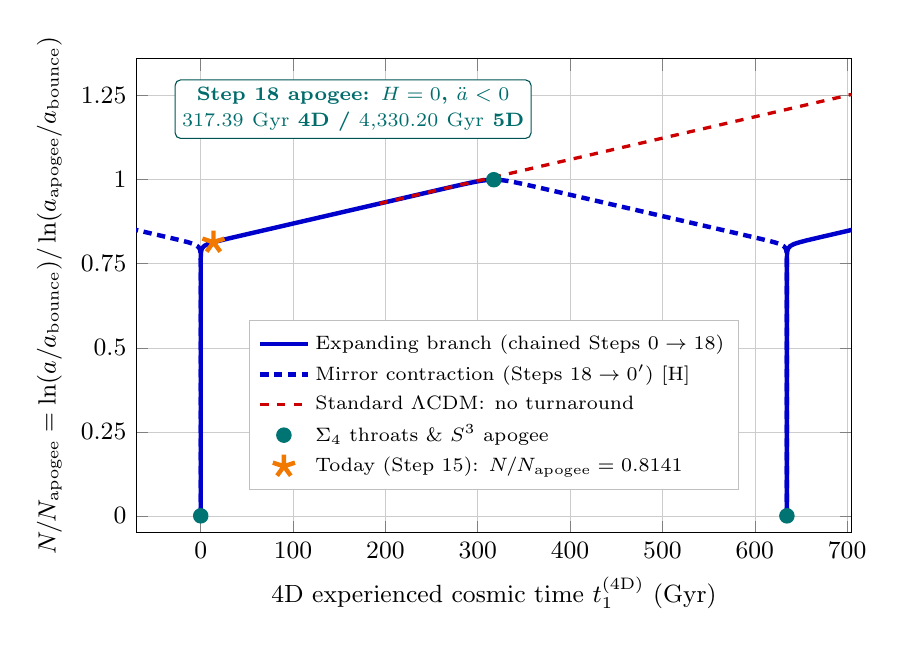
\begin{tikzpicture}
\begin{axis}[
    width=0.88\textwidth,
    height=7.6cm,
    xlabel={4D experienced cosmic time $t_1^{\mathrm{(4D)}}$ (Gyr)},
    ylabel={$N/N_{\mathrm{apogee}} = \ln(a/a_{\mathrm{bounce}})/\ln(a_{\mathrm{apogee}}/a_{\mathrm{bounce}})$},
    xmin=-70, xmax=705,
    ymin=-0.05, ymax=1.36,
    xtick={0, 100, 200, 300, 400, 500, 600, 700},
    ytick={0.0, 0.25, 0.50, 0.75, 1.00, 1.25},
    grid=both,
    grid style={line width=.1pt, draw=gray!20},
    major grid style={line width=.2pt, draw=gray!40},
    legend style={at={(0.5,0.09)}, anchor=south, font=\scriptsize, fill=white, draw=gray!50, cells={anchor=west}, inner sep=3pt},
    tick label style={font=\small},
    xlabel style={font=\small},
    ylabel style={font=\small}
]
% Expanding branch (chained Steps 0 -> 18) and its copy in the next cycle
\addplot[ultra thick, blue!80!black] coordinates {
    (0.0000, 0.00000) (0.0000, 0.66917) (0.0000, 0.71378) (0.0004, 0.73608) (0.0019, 0.74724) (0.0091, 0.75839)
    (0.0421, 0.76954) (0.0897, 0.77512) (0.1908, 0.78069) (0.4051, 0.78627) (0.8586, 0.79185) (1.8141, 0.79742)
    (3.7919, 0.80300) (7.6216, 0.80858) (13.7909, 0.81411) (21.7542, 0.81973) (30.3101, 0.82530) (39.0364, 0.83088)
    (47.8024, 0.83646) (65.3542, 0.84761) (82.9089, 0.85876) (100.4639, 0.86992) (118.0188, 0.88107) (135.5738, 0.89222)
    (153.1287, 0.90337) (170.6836, 0.91453) (188.2386, 0.92568) (193.5833, 0.92908) (205.7936, 0.93683) (223.3488, 0.94799)
    (240.9063, 0.95914) (258.4797, 0.97029) (267.2940, 0.97587) (276.1729, 0.98144) (283.3967, 0.98590) (290.8950, 0.99037)
    (296.9571, 0.99371) (301.4930, 0.99594) (305.4973, 0.99762) (308.8553, 0.99873) (312.1555, 0.99951) (314.4680, 0.99985)
    (317.3898, 1.00000)
};
\addlegendentry{Expanding branch (chained Steps $0 \rightarrow 18$)}
\addplot[ultra thick, blue!80!black, forget plot] coordinates {
    (634.7795, 0.00000) (634.7795, 0.66917) (634.7795, 0.71378) (634.7799, 0.73608) (634.7814, 0.74724) (634.7886, 0.75839)
    (634.8216, 0.76954) (634.8692, 0.77512) (634.9703, 0.78069) (635.1846, 0.78627) (635.6381, 0.79185) (636.5936, 0.79742)
    (638.5714, 0.80300) (642.4011, 0.80858) (648.5704, 0.81411) (656.5337, 0.81973) (665.0896, 0.82530) (673.8159, 0.83088)
    (682.5819, 0.83646) (700.1337, 0.84761) (717.6884, 0.85876) (735.2434, 0.86992) (752.7983, 0.88107)
};
% Contracting branch: apogee time-reflection mirror t -> T_cycle - t [H] (and the previous cycle for t < 0)
\addplot[ultra thick, blue!80!black, densely dashed] coordinates {
    (634.7795, 0.00000) (634.7795, 0.66917) (634.7795, 0.71378) (634.7791, 0.73608) (634.7776, 0.74724) (634.7704, 0.75839)
    (634.7374, 0.76954) (634.6898, 0.77512) (634.5887, 0.78069) (634.3744, 0.78627) (633.9209, 0.79185) (632.9654, 0.79742)
    (630.9876, 0.80300) (627.1579, 0.80858) (620.9886, 0.81411) (613.0253, 0.81973) (604.4694, 0.82530) (595.7431, 0.83088)
    (586.9771, 0.83646) (569.4253, 0.84761) (551.8706, 0.85876) (534.3156, 0.86992) (516.7607, 0.88107) (499.2057, 0.89222)
    (481.6508, 0.90337) (464.0959, 0.91453) (446.5409, 0.92568) (441.1962, 0.92908) (428.9859, 0.93683) (411.4307, 0.94799)
    (393.8732, 0.95914) (376.2998, 0.97029) (367.4855, 0.97587) (358.6066, 0.98144) (351.3828, 0.98590) (343.8845, 0.99037)
    (337.8224, 0.99371) (333.2865, 0.99594) (329.2822, 0.99762) (325.9242, 0.99873) (322.6240, 0.99951) (320.3115, 0.99985)
    (317.3897, 1.00000)
};
\addlegendentry{Mirror contraction (Steps $18 \rightarrow 0'$) [H]}
\addplot[ultra thick, blue!80!black, densely dashed, forget plot] coordinates {
    (-0.0000, 0.00000) (-0.0000, 0.66917) (-0.0000, 0.71378) (-0.0004, 0.73608) (-0.0019, 0.74724) (-0.0091, 0.75839)
    (-0.0421, 0.76954) (-0.0897, 0.77512) (-0.1908, 0.78069) (-0.4051, 0.78627) (-0.8586, 0.79185) (-1.8141, 0.79742)
    (-3.7919, 0.80300) (-7.6216, 0.80858) (-13.7909, 0.81411) (-21.7542, 0.81973) (-30.3101, 0.82530) (-39.0364, 0.83088)
    (-47.8024, 0.83646) (-65.3542, 0.84761) (-82.9089, 0.85876) (-100.4639, 0.86992)
};
% Standard LambdaCDM: de Sitter growth dN/dt = H_Lambda continues without turnaround
\addplot[very thick, dashed, red!80!black] coordinates {(193.5833, 0.92908) (705, 1.25398)};
\addlegendentry{Standard $\Lambda\text{CDM}$: no turnaround}
% Landmarks
\addplot[only marks, mark=*, mark size=2.6pt, teal!90!black] coordinates {(0.0, 0.0) (317.3898, 1.0) (634.7795, 0.0)};
\addlegendentry{$\Sigma_4$ throats \& $S^3$ apogee}
\addplot[only marks, mark=star, mark size=4.2pt, ultra thick, orange!95!black] coordinates {(13.7909, 0.81411)};
\addlegendentry{Today (Step 15): $N/N_{\mathrm{apogee}} = 0.8141$}
\node[font=\scriptsize\bfseries, text=teal!85!black, fill=white, draw=teal!65!black, rounded corners=2pt, inner sep=2.5pt] at (axis cs: 165, 1.21) {\shortstack{Step 18 apogee: $H = 0$, $\ddot{a} < 0$\\$317.39\mathrm{~Gyr}$ 4D / $4{,}330.20\mathrm{~Gyr}$ 5D}};
\end{axis}
\end{tikzpicture}
\caption{Global macro-chronology of the chained 18-step $S^3$ Holonomy Apogee cycle~(\ref{eq:exact_restitution_friedmann})--(\ref{eq:exact_turnaround_time}) (\catD/\catH/\catN, Checks~\texttt{\#104}--\texttt{\#112}, \texttt{\#139}--\texttt{\#152}): the computed trajectory in the e-folding coordinate $N/N_{\text{apogee}}$ against linear 4D time, showing the expanding branch (solid), the apogee time-reflection mirror branch \catH\ (dashed), the continuation of standard $\Lambda\text{CDM}$ (dashed red), the present cosmos at Step~15 ($t_0^{\text{(4D)}} = 13.7909\text{ Gyr}, t_0^{\text{(5D)}} = 188.15\text{ Gyr}$, orange star), the global $S^3$ Holonomy Apogee ($t_{\text{apogee}}^{\text{(4D)}} = 317.39\text{ Gyr}, t_{\text{apogee}}^{\text{(5D)}} = 4{,}330.20\text{ Gyr}, a_{\text{apogee}} = \Phi_{\infty}^{-2} = 1.7320 \times 10^7$) and the $\Sigma_4$ bounce throats at $t_1 = t_P$ and $T_{\text{cycle}}^{\text{(4D)}} = 634.78\text{ Gyr}$. The three apparent corners of this curve (the throats, the ``elbow'' near $14\text{ Gyr}$ and the apogee) are artefacts of the $700\text{ Gyr}$ horizontal scale, on which $73.0$ of the $89.66$ e-folds elapse in the first $13.79\text{ Gyr}$; each is resolved as a smooth $\mathcal{C}^{\infty}$ curve in the companion zooms of Fig.~\ref{fig:cyclic_universe_zooms}.}
\label{fig:cyclic_universe_trajectory}
\end{figure}

\begin{figure}[H]
\centering
% Coordinates computed from the locked integrator of verify_cbg_paper3_v13.py (step1_odes_tau, step_N_odes, Step 18 regular-time leg)
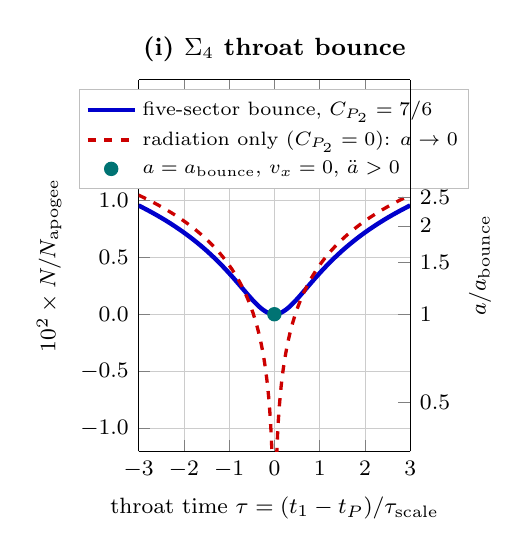
\begin{tikzpicture}
\begin{axis}[
    width=0.415\textwidth,
    height=6.3cm,
    title={(i) $\Sigma_4$ throat bounce},
    title style={font=\small\bfseries, yshift=-3pt},
    xlabel={throat time $\tau = (t_1 - t_P)/\tau_{\mathrm{scale}}$},
    ylabel={$10^{2} \times N/N_{\mathrm{apogee}}$},
    xmin=-3, xmax=3,
    ymin=-1.2, ymax=2.05,
    xtick={-3, -2, -1, 0, 1, 2, 3},
    ytick={-1.0, -0.5, 0.0, 0.5, 1.0},
    yticklabel style={/pgf/number format/fixed, /pgf/number format/precision=1, /pgf/number format/fixed zerofill},
    axis y line*=left,
    grid=both,
    grid style={line width=.1pt, draw=gray!20},
    major grid style={line width=.2pt, draw=gray!40},
    legend style={at={(0.5,0.975)}, anchor=north, font=\scriptsize, fill=white, draw=gray!50, cells={anchor=west}, inner sep=2pt},
    tick label style={font=\footnotesize},
    xlabel style={font=\footnotesize},
    ylabel style={font=\footnotesize}
]
\addplot[ultra thick, blue!80!black] coordinates {
    (-3.000, 0.95148) (-2.900, 0.93137) (-2.800, 0.91061) (-2.700, 0.88914) (-2.600, 0.86693)
    (-2.500, 0.84392) (-2.400, 0.82007) (-2.300, 0.79531) (-2.200, 0.76960) (-2.100, 0.74286)
    (-2.000, 0.71502) (-1.900, 0.68602) (-1.800, 0.65577) (-1.700, 0.62418) (-1.600, 0.59118)
    (-1.500, 0.55668) (-1.400, 0.52060) (-1.300, 0.48287) (-1.200, 0.44345) (-1.100, 0.40232)
    (-1.000, 0.35953) (-0.900, 0.31523) (-0.800, 0.26970) (-0.700, 0.22346) (-0.600, 0.17730)
    (-0.550, 0.15462) (-0.500, 0.13245) (-0.450, 0.11102) (-0.400, 0.09060) (-0.350, 0.07147)
    (-0.300, 0.05395) (-0.250, 0.03837) (-0.200, 0.02506) (-0.150, 0.01433) (-0.100, 0.00644)
    (-0.050, 0.00162) (0.000, 0.00000) (0.050, 0.00162) (0.100, 0.00644) (0.150, 0.01433)
    (0.200, 0.02506) (0.250, 0.03837) (0.300, 0.05395) (0.350, 0.07147) (0.400, 0.09060)
    (0.450, 0.11102) (0.500, 0.13245) (0.550, 0.15462) (0.600, 0.17730) (0.700, 0.22346)
    (0.800, 0.26970) (0.900, 0.31523) (1.000, 0.35953) (1.100, 0.40232) (1.200, 0.44345)
    (1.300, 0.48287) (1.400, 0.52060) (1.500, 0.55668) (1.600, 0.59118) (1.700, 0.62418)
    (1.800, 0.65577) (1.900, 0.68602) (2.000, 0.71502) (2.100, 0.74286) (2.200, 0.76960)
    (2.300, 0.79531) (2.400, 0.82007) (2.500, 0.84392) (2.600, 0.86693) (2.700, 0.88914)
    (2.800, 0.91061) (2.900, 0.93137) (3.000, 0.95148)
};
\addlegendentry{five-sector bounce, $C_{P_2} = 7/6$}
\addplot[domain=-3:-0.05, samples=151, very thick, dashed, red!80!black] {100*ln(sqrt(2.160247*abs(x)))/89.66382};
\addlegendentry{radiation only ($C_{P_2} = 0$): $a \rightarrow 0$}
\addplot[domain=0.05:3, samples=151, very thick, dashed, red!80!black, forget plot] {100*ln(sqrt(2.160247*abs(x)))/89.66382};
\addplot[only marks, mark=*, mark size=2.4pt, teal!90!black] coordinates {(0.0, 0.0)};
\addlegendentry{$a = a_{\mathrm{bounce}}$, $v_x = 0$, $\ddot{a} > 0$}
\end{axis}
\begin{axis}[
    width=0.415\textwidth,
    height=6.3cm,
    xmin=-3, xmax=3,
    ymin=-1.2, ymax=2.05,
    axis x line=none,
    axis y line*=right,
    ytick={-0.77306, 0.0, 0.45221, 0.77306, 1.02192},
    yticklabels={$0.5$, $1$, $1.5$, $2$, $2.5$},
    ylabel={$a/a_{\mathrm{bounce}}$},
    tick label style={font=\footnotesize},
    ylabel style={font=\footnotesize}
]
\end{axis}
\end{tikzpicture}\hfill
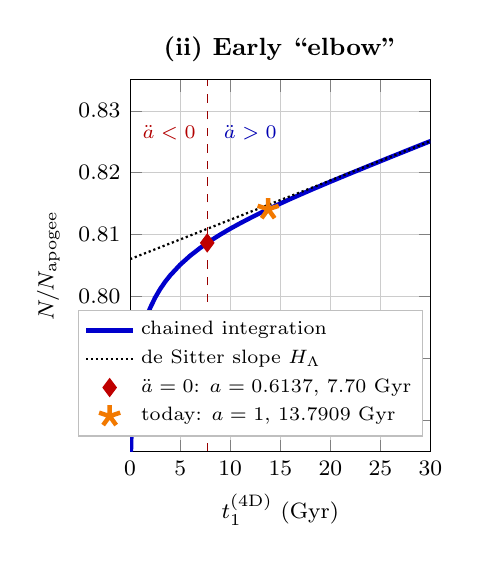
\begin{tikzpicture}
\begin{axis}[
    width=0.445\textwidth,
    height=6.3cm,
    title={(ii) Early ``elbow''},
    title style={font=\small\bfseries, yshift=-3pt},
    xlabel={$t_1^{\mathrm{(4D)}}$ (Gyr)},
    ylabel={$N/N_{\mathrm{apogee}}$},
    xmin=0, xmax=30,
    ymin=0.775, ymax=0.835,
    xtick={0, 5, 10, 15, 20, 25, 30},
    ytick={0.78, 0.79, 0.80, 0.81, 0.82, 0.83},
    yticklabel style={/pgf/number format/fixed, /pgf/number format/precision=2, /pgf/number format/fixed zerofill},
    grid=both,
    grid style={line width=.1pt, draw=gray!20},
    major grid style={line width=.2pt, draw=gray!40},
    legend style={at={(0.975,0.04)}, anchor=south east, font=\scriptsize, fill=white, draw=gray!50, cells={anchor=west}, inner sep=2pt},
    tick label style={font=\footnotesize},
    xlabel style={font=\footnotesize},
    ylabel style={font=\footnotesize}
]
\addplot[ultra thick, blue!80!black] coordinates {
    (0.0700, 0.77329) (0.1000, 0.77592) (0.1500, 0.77891) (0.2000, 0.78104) (0.3000, 0.78404)
    (0.4000, 0.78618) (0.5500, 0.78854) (0.7000, 0.79033) (0.9000, 0.79220) (1.1000, 0.79369)
    (1.4000, 0.79549) (1.7000, 0.79694) (2.0000, 0.79815) (2.5000, 0.79983) (3.0000, 0.80121)
    (3.5000, 0.80239) (4.0000, 0.80341) (5.0000, 0.80515) (6.0000, 0.80660) (7.0000, 0.80786)
    (8.0000, 0.80899) (9.0000, 0.81001) (10.0000, 0.81096) (11.0000, 0.81185) (12.0000, 0.81269)
    (13.0000, 0.81350) (13.7909, 0.81411) (15.0000, 0.81502) (16.0000, 0.81576) (17.0000, 0.81647)
    (18.0000, 0.81718) (20.0000, 0.81855) (22.0000, 0.81989) (24.0000, 0.82121) (26.0000, 0.82252)
    (28.0000, 0.82382) (30.0000, 0.82511)
};
\addlegendentry{chained integration}
\addplot[thick, densely dotted, black] coordinates {(0, 0.80605) (30, 0.82511)};
\addlegendentry{de Sitter slope $H_{\Lambda}$}
\addplot[only marks, mark=diamond*, mark size=3.2pt, red!75!black] coordinates {(7.7043, 0.80867)};
\addlegendentry{$\ddot{a} = 0$: $a = 0.6137$, $7.70\mathrm{~Gyr}$}
\addplot[only marks, mark=star, mark size=4.0pt, ultra thick, orange!95!black] coordinates {(13.7909, 0.81411)};
\addlegendentry{today: $a = 1$, $13.7909\mathrm{~Gyr}$}
\node[font=\scriptsize, text=red!70!black] at (axis cs: 3.9, 0.8265) {$\ddot{a} < 0$};
\node[font=\scriptsize, text=blue!70!black] at (axis cs: 12.0, 0.8265) {$\ddot{a} > 0$};
\addplot[thin, dashed, red!60!black, forget plot] coordinates {(7.7043, 0.775) (7.7043, 0.835)};
\end{axis}
\end{tikzpicture}

\vspace{4pt}
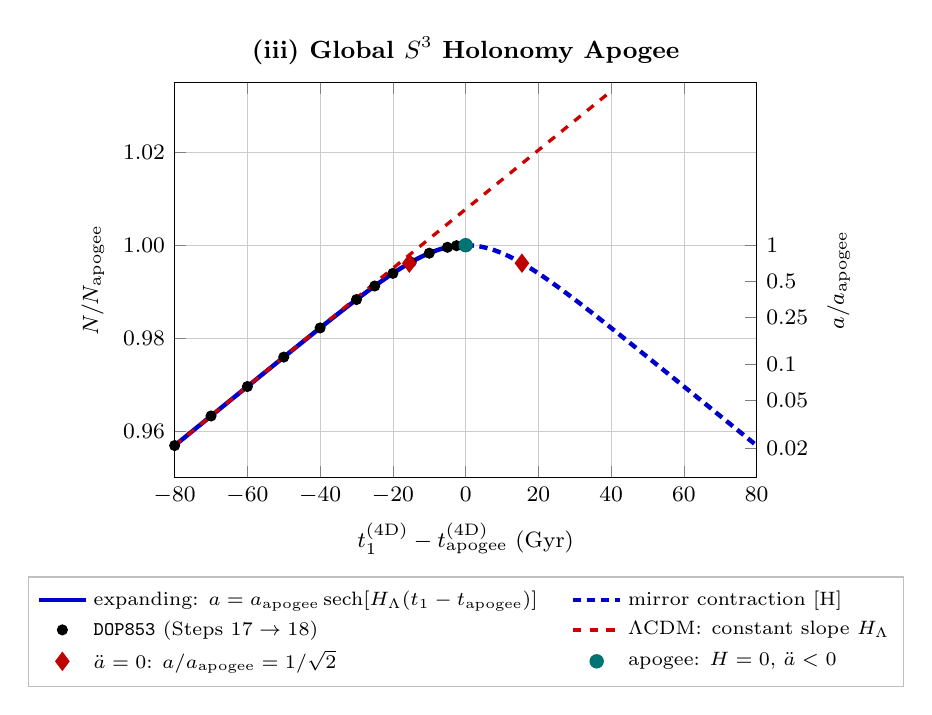
\begin{tikzpicture}
\begin{axis}[
    width=0.74\textwidth,
    height=6.6cm,
    title={(iii) Global $S^3$ Holonomy Apogee},
    title style={font=\small\bfseries, yshift=-3pt},
    xlabel={$t_1^{\mathrm{(4D)}} - t_{\mathrm{apogee}}^{\mathrm{(4D)}}$ (Gyr)},
    ylabel={$N/N_{\mathrm{apogee}}$},
    xmin=-80, xmax=80,
    ymin=0.950, ymax=1.035,
    xtick={-80, -60, -40, -20, 0, 20, 40, 60, 80},
    ytick={0.96, 0.98, 1.00, 1.02},
    yticklabel style={/pgf/number format/fixed, /pgf/number format/precision=2, /pgf/number format/fixed zerofill},
    axis y line*=left,
    grid=both,
    grid style={line width=.1pt, draw=gray!20},
    major grid style={line width=.2pt, draw=gray!40},
    legend columns=2,
    legend style={at={(0.5,-0.25)}, anchor=north, font=\scriptsize, fill=white, draw=gray!50, cells={anchor=west}, inner sep=3pt, /tikz/every even column/.append style={column sep=10pt}},
    tick label style={font=\footnotesize},
    xlabel style={font=\footnotesize},
    ylabel style={font=\footnotesize}
]
\addplot[domain=-80:0, samples=121, ultra thick, blue!80!black] {1 - ln(cosh(0.056964*x))/89.66382};
\addlegendentry{expanding: $a = a_{\mathrm{apogee}}\operatorname{sech}[H_{\Lambda}(t_1 - t_{\mathrm{apogee}})]$}
\addplot[domain=0:80, samples=121, ultra thick, blue!80!black, densely dashed] {1 - ln(cosh(0.056964*x))/89.66382};
\addlegendentry{mirror contraction [H]}
\addplot[only marks, mark=*, mark size=1.8pt, black] coordinates {
    (-80.0, 0.95690) (-70.0, 0.96326) (-60.0, 0.96960) (-50.0, 0.97593) (-40.0, 0.98220)
    (-30.0, 0.98831) (-25.0, 0.99122) (-20.0, 0.99394) (-15.0, 0.99634) (-10.0, 0.99828)
    (-5.0, 0.99955) (-2.5, 0.99989) (0.0, 1.00000)
};
\addlegendentry{\texttt{DOP853} (Steps $17 \rightarrow 18$)}
\addplot[domain=-80:40, samples=2, very thick, dashed, red!80!black] {1 + (0.693147 + 0.056964*x)/89.66382};
\addlegendentry{$\Lambda\text{CDM}$: constant slope $H_{\Lambda}$}
\addplot[only marks, mark=diamond*, mark size=3.2pt, red!75!black] coordinates {(-15.47, 0.99613) (15.47, 0.99613)};
\addlegendentry{$\ddot{a} = 0$: $a/a_{\mathrm{apogee}} = 1/\sqrt{2}$}
\addplot[only marks, mark=*, mark size=2.4pt, teal!90!black] coordinates {(0.0, 1.0)};
\addlegendentry{apogee: $H = 0$, $\ddot{a} < 0$}
\end{axis}
\begin{axis}[
    width=0.74\textwidth,
    height=6.6cm,
    xmin=-80, xmax=80,
    ymin=0.950, ymax=1.035,
    axis x line=none,
    axis y line*=right,
    ytick={0.95637, 0.96659, 0.97432, 0.98454, 0.99227, 1.0},
    yticklabels={$0.02$, $0.05$, $0.1$, $0.25$, $0.5$, $1$},
    ylabel={$a/a_{\mathrm{apogee}}$},
    tick label style={font=\footnotesize},
    ylabel style={font=\footnotesize}
]
\end{axis}
\end{tikzpicture}
\caption{$\mathcal{C}^{\infty}$ resolution of the three apparent corners of Fig.~\ref{fig:cyclic_universe_trajectory}, in the same e-folding coordinate $N/N_{\text{apogee}}$ (left axes; the physical size is on the right axes of Panels~(i) and (iii)), with coordinates computed from the integrator of \texttt{verify\_cbg\_paper3\_v13.py}. Panel~(i): the $\Sigma_4$ throat in dimensionless throat time, where the constitutive five-sector model \catH\ gives a smooth rebound at $x(0) = a/a_{\text{bounce}} = 1$, $v_x(0) = 0$ with $dv_x/d\tau|_0 = -(1 + \widetilde{\mathcal{V}}(\psi_b)/6) + 2C_{P_2} \simeq +7/6 > 0$ ($D_{\text{obs},b} = 17.33\,\mu\text{m}$; $\tau < 0$ by the time-reversal invariance of Check~\texttt{\#139}), contrasted with the radiation-only solution $x = (2\sqrt{7/6}\,|\tau|)^{1/2}$ without the recoil sector, which reaches $a = 0$. Panel~(ii): the first $30\text{ Gyr}$, where the trajectory passes smoothly from decelerated expansion ($\ddot{a} < 0$) to the constant-slope de Sitter regime ($\ddot{a} > 0$) through the acceleration-inversion point $a = 0.6137$ at $t_1^{\text{(4D)}} \approx 7.70\text{ Gyr}$ (Check~\texttt{\#143}), with the present cosmos at Step~15 ($a = 1$, $t_0^{\text{(4D)}} = 13.7909\text{ Gyr}$, $N/N_{\text{apogee}} = 0.8141$, Check~\texttt{\#107}). Panel~(iii): $\pm 80\text{ Gyr}$ around the apogee at $317.39\text{ Gyr}$, a smooth turning point ($H = 0$, $\ddot{a} < 0$) following $a = a_{\text{apogee}}\operatorname{sech}[H_{\Lambda}(t_1 - t_{\text{apogee}})]$ with the \texttt{DOP853} points on it, the mirror contraction \catH, the constant-slope $\Lambda\text{CDM}$ continuation, and the braking inflections $\ddot{a} = 0$ at $a/a_{\text{apogee}} = 1/\sqrt{2}$, $15.47\text{ Gyr}$ either side of the apogee ($301.92\text{ Gyr}$ and $332.86\text{ Gyr}$, Checks~\texttt{\#144}--\texttt{\#145}). The last $3.9$ e-folds before the apogee are a small step in $N/N_{\text{apogee}}$ (from $0.957$ at $-80\text{ Gyr}$) but a factor of $48$ in size ($a/a_{\text{apogee}} = 0.021$ there), because $1/H_{\Lambda} = 17.55\text{ Gyr} \ll T_{\text{cycle}}^{\text{(4D)}}$.}
\label{fig:cyclic_universe_zooms}
\end{figure}

% ============================================================================
% SECTION 10: MASTER SYNTHESIS OF COSMOLOGICAL PREDICTIONS & BENCHMARKS
% ============================================================================
\section{\texorpdfstring{Master Synthesis of Cosmological Predictions, the 19-Point Chained Chronology Table (Steps~$0 \to 18$), and Observational Roadmap (2026--2035) (\catA/\catD/\catH/\catN)}{Master Synthesis of Cosmological Predictions, the 19-Point Chained Chronology Table (Steps 0 -> 18), and Observational Roadmap (2026-2035)}}

\subsection{\texorpdfstring{Unified Overview Across Sixty-Three Orders of Magnitude in Cosmic Time}{Unified Overview Across Sixty-Three Orders of Magnitude in Cosmic Time}}

Across the cosmological and astrophysical regimes analyzed in this monograph---from the exact three-equation $k = +1$ ($\mathcal{S}_{t_2} \times S^3$) breathing bounce (\catD) and the $\Sigma_4$ Bekenstein--Hermite bounce throat ($t_1 = t_P = 5.3912 \times 10^{-44}\text{ s}, D_{\text{obs},b} = 17.33\,\mu\text{m}, V_{S^3} = 28.90\text{ cm}^3, \Delta\Pi_2 = 1/54, \Delta_{\text{IR}} = -17$, Step~0 \catD/\catH) through CMB recombination (Step~12, $t_{12}^{\text{(4D)}} = 369.2\text{ kyr}, t_{12}^{\text{(5D)}} = 5.037\text{ Myr}, z_*^{\text{(CBG)}} = 1093.99$), the UV/IR dilaton bath and JWST quasar seed epoch (Step~14, $z_\chi = 16.84, t_{14}^{\text{(4D)}} = 227.0\text{ Myr}, t_{14}^{\text{(5D)}} = 3.097\text{ Gyr}$), the present cosmos (Step~15, $z = 0, a = 1, t_0^{\text{(4D)}} = 13.7909\text{ Gyr}, t_0^{\text{(5D)}} = 188.15\text{ Gyr}$), and the global $S^3$ Holonomy Apogee (Step~18, $a_{\text{apogee}} = \Phi_{\infty}^{-2} = 1.7320 \times 10^7, t_{\text{apogee}}^{\text{(4D)}} = 317.39\text{ Gyr}, t_{\text{apogee}}^{\text{(5D)}} = 4{,}330.20\text{ Gyr}, T_{\text{cycle}}^{\text{(4D)}} = 634.78\text{ Gyr}, T_{\text{cycle}}^{\text{(5D)}} = 8{,}660.41\text{ Gyr}$ \catH/\catN)---all derivations and benchmarks are anchored by the integer invariants $(d_t, d_s, D) = (2, 3, 5)$ ($\operatorname{End}(V_5) = 13_+ \oplus 12_-$, $\mathcal{N}_{\text{Cartan}} = 30$, $\mathcal{D}_{\text{config}} = 17$) and the vacuum fiber and horizon constants established in \textit{Paper~0} (\textit{Principia Geometrica} \cite{jimenez2026_p0}), \textit{Paper~I} (v12 \cite{jimenez2026a}), and \textit{Paper~II} (v12 \cite{jimenez2026b}):
\begin{align}
\Phi_{\infty} &= 2.40286677 \times 10^{-4} \;\;\catD/\catH/\catN, \qquad \Phi_{\infty}^2 = 5.773769 \times 10^{-8}, \nonumber \\[3pt]
\Omega_{\infty} &= c\Phi_{\infty} = 72.0361\text{ km/s} \;\; \left(72{,}036.13\text{ m/s}\right) \;\;\catD/\catH, \nonumber \\[3pt]
\eta_{\text{bitemp}} &= 13\left(1 + \Omega_{b,0}\right) = 13.643175 \;\;\catD/\catH, \nonumber \\[3pt]
a_0^{\text{(dS)}} &= \frac{cH_0}{2\pi} = 1.0422 \times 10^{-10}\text{ m/s}^2 \;\;\catN, \nonumber \\[3pt]
a_0^{\text{(CBG)}} &= \frac{17}{15}\frac{cH_0}{2\pi} = 1.1812 \times 10^{-10}\text{ m/s}^2 \;\;\catD/\catH/\catN.
\label{eq:master_synthesis_constants_p3}
\end{align}
Table~\ref{tab:master_cosmological_observables} synthesizes the analytical formulas, numerical values, and strict epistemological classifications (\catA, \catD, \catH, \catN) across this monograph, while Table~\ref{tab:complete_cosmic_chronology} records the complete 19-point chained dynamical trajectory across Steps~$0 \to 18$ verified with Hamiltonian constraint (Steps~0--1, 18) and ODE-independent 4th-order finite-difference trajectory (Steps~2--17) residuals $\le 6.97 \times 10^{-11}$ (Check~\texttt{\#104}) in \allowbreak\texttt{verify\_cbg\_paper3\_v13.py}.

\begin{table}[H]
\centering
\caption{Master Summary of Cosmological Results, Postulated Models, and Empirical Scaling Benchmarks (\catA, \catD, \catH, \catN) in Covariant Bitemporal Geometrodynamics (Paper~III, v13 Deductive Bundle Edition, Verified by \texttt{verify\_cbg\_paper3\_v13.py}, 157/157 PASSED).}
\label{tab:master_cosmological_observables}
\vspace{0.10cm}
\footnotesize
\setlength{\tabcolsep}{3.5pt}
\renewcommand{\arraystretch}{1.22}
\begin{tabularx}{\textwidth}{@{} L{0.20\textwidth} C{0.11\textwidth} C{0.22\textwidth} C{0.18\textwidth} Y @{}}
\toprule
\textbf{Cosmological / Gravitational Quantity} & \textbf{Class} & \textbf{Analytical Formula} & \textbf{Numerical Value} & \textbf{Physical Scope \& Observational Test} \\
\midrule
\textbf{1. $k=+1$ Bounce \& Shear Model} & \catD/\catH & $\left.\dfrac{\ddot{a}}{a_b}\right|_{H=0} = \dfrac{V_{\psi} - \rho_r - 2\rho_{\sigma}}{3}$,\newline$\ddot{\psi}(0) = \dfrac{2(V-V_{\psi})}{3}$ & $\mathbf{+0.3000\,m_{\psi}^2}$ (\catD),\newline$\mathbf{-0.7200\,m_{\psi}^2}$ & Exact isotropic $k=+1$ bounce \catD; shear-fluid model $+0.20\,m_{\psi}^2$ \catD/\catH\ (Checks~\texttt{\#026}--\texttt{\#027}, \texttt{\#038}--\texttt{\#065}) \\
\addlinespace[2.5pt]
\textbf{2. 5D Bianchi-I ($k=0$) Shear Law} & \catD & $\dfrac{d}{dt_1}\!\left(a^3\Phi\sigma^i_{\;j}\right) = 0$ & $\rho_{\sigma} = \dfrac{\Sigma_0^2}{a^6 e^{2\psi}}$ & Metric-first 5D Bianchi-I conservation law (Checks~\texttt{\#021}--\texttt{\#025}, Thm.~\ref{thm:bkl_shear_suppression}) \\
\addlinespace[2.5pt]
\textbf{3. $\Pi_2(\psi)$ Barrier \& 5-Sector Noether} & \catD & $\Delta\Pi_2 = \dfrac{1}{d_t d_s^3}$,\newline$\dfrac{d\mathcal{E}_N}{d\tau} + 2H_d\mathcal{E}_N \equiv 0$ & $\mathbf{\dfrac{1}{54}}$, $\lambda_{\text{UV}} = \mathbf{+0.3238}$,\newline$\mathbf{\Delta_{\text{IR}} = -17}$ & Exact symbolic proofs at $\psi_{\max}^{\text{(BH)}}=\frac{1}{2}\ln 3$ and $\psi=0$ (Checks~\texttt{\#028}--\texttt{\#032}, Thms.~\ref{thm:bekenstein_hermite_barrier_p3}--\ref{thm:five_sector_bianchi_noether_p3}) \\
\addlinespace[2.5pt]
\textbf{4. Pure 5D $\alpha_0^2 = 1/3$ \& BH Hair} & \catD & $\alpha_0^2 = \dfrac{c_{\text{Weyl}}^2}{-2\kappa_{\psi}} = -c_{\text{DW}}^{-1}$,\newline$B = 1 + \dfrac{r(1+2A\psi_t')A'}{A} + \dots$ & $\mathbf{\alpha_{\text{Yuk}}=\dfrac{1}{3}}$,\newline$\mathbf{f_{\text{hair}} = 4.162\%}$, $\mathbf{-8.151\%}$ & $15\times 15$ DeWitt + Weyl proof (\texttt{\#008}--\texttt{\#011}); monotone $r_{\max}=60$ BVP (\texttt{\#033}--\texttt{\#034}, \texttt{\#068}--\texttt{\#086}) \\
\addlinespace[2.5pt]
\textbf{5. Sub-$50\,\mu\text{m}$ E\"ot-Wash / HUST} & \catD/\catH/\catN & $\alpha_{\text{Yuk}} = \dfrac{1}{3}$,\newline$\lambda_{\text{micro}} = \sqrt{L_P R_H}$ & $\mathbf{47 \pm 2\,\mu\text{m}}$\newline($m_{\psi} = \mathbf{4.19\text{ meV}}$) & Factor $\sim 1.5\text{--}1.8$ below E\"ot-Wash 2020 \& HUST 2020 bounds (Checks~\texttt{\#123}--\texttt{\#124}) \cite{lee2020,tan2020_hust} \\
\addlinespace[2.5pt]
\textbf{6. Chained 18-Step Ages \& Apogee} & \catD/\catH/\catN & $t_0^{\text{(5D)}} = \eta_{\text{bitemp}}t_0^{\text{(4D)}}$,\newline$a_{\text{apogee}} = \Phi_{\infty}^{-2}$ & $\mathbf{13.7909\text{ Gyr}}$ 4D\newline($\mathbf{188.15\text{ Gyr}}$ 5D) & Apogee $a=1.7320\times 10^7$ at $317.39\text{ Gyr}$ 4D / $4{,}330.20\text{ Gyr}$ 5D, $|\mathcal{E}_N|$/FD res.\ $\le 6.97\times 10^{-11}$ (\texttt{\#094}--\texttt{\#112}) \\
\addlinespace[2.5pt]
\textbf{7. Birefringence ($\beta_{\text{CMB}}, \beta_{\text{reion}}$)} & \catH & $+180^\circ\,\Phi_{\infty}\ln\left(1 + z\right)$ & $\mathbf{+0.3025^\circ}$ /\newline$\mathbf{+0.0936^\circ}$ & Matches \textit{Planck} PR4 $+0.30^\circ$; LiteBIRD discriminator vs.\ $\psi F\tilde{F}$ (Checks~\texttt{\#087}--\texttt{\#093}) \\
\addlinespace[2.5pt]
\textbf{8. 5D Oscillating-$\psi$ Condensate} & \catD/\catH & $\langle w_{\psi}\rangle = 0$,\newline$\langle\rho_{\psi}\rangle \propto a^{-3}$ & $|\langle w_{\psi}\rangle| = 6.1\times 10^{-8}$\newline(\texttt{\#066}--\texttt{\#067}) & Direct 5D \texttt{DOP853}+\texttt{brentq} proof; reproduces $\Lambda\text{CDM}$ \texttt{CLASS} TT/EE peaks (Sec.~6.1) \\
\addlinespace[2.5pt]
\textbf{9. Planck Remnants \& JWST Seeds} & \catD/\catH & $M_{\text{rem}} = \dfrac{m_P}{2}$,\newline$\tau_{\text{Salp}}^{\text{(CBG)}} = \dfrac{3}{4}\tau_{\text{Salp}}^{\text{(GR)}}$ & $\mathbf{33.75\text{ Myr}}$\newline($\mathbf{12.89\text{ e-folds}}$) & Grows $100\,M_{\odot}$ seed to $3.96\times 10^7\,M_{\odot}$ (UHZ1 \& GN-z11, Checks~\texttt{\#113}--\texttt{\#115}) \\
\addlinespace[2.5pt]
\textbf{10. Reheating, $\eta_B$ \& $N_{\text{rad}}$} & \catD/\catN & $\frac{1}{4}\ln(\rho_P/\rho_{\text{eq}})$,\newline$\chi_{\text{loop}}\Phi_{\infty}^2 E_P$ & $\mathbf{64.70}$, $\mathbf{704.91\text{ PeV}}$,\newline$\mathbf{6.109 \times 10^{-10}}$ & Exact $N_{\text{rad}}$ \catD\ (Check~\texttt{\#117}); $\widetilde{E}_1$ \& $\eta_B$ within $0.27\sigma$ of \textit{Planck} (\texttt{\#120}--\texttt{\#122}) \\
\addlinespace[2.5pt]
\textbf{11. Horizon Ratios \& Matter ($\Omega_{m,\text{eff}}$)} & \catN & $\dfrac{\Phi_{\infty}}{4\pi}, \;\dfrac{\Phi_{\infty}^2}{8\pi}$,\newline$\sqrt{\dfrac{2\pi}{3}\Omega_{b,0}}$ & $\mathbf{2.297 \times 10^{-9}}$,\newline$\mathbf{0.32133}$ & $\Omega_{m,0}^{\text{(mode)}} = 0.31589$ (Check~\texttt{\#095}); $\mathcal{F}^{\text{(proj)}} = 5.4353$, WKB $\mathcal{H}_{3/2} = 0.990$ (\texttt{\#125}--\texttt{\#134}) \\
\addlinespace[2.5pt]
\textbf{12. Local $H_0$ \& Volumetric $(w_0, w_a)$} & \catN/\catH & $H_0(1+\Omega_{\infty}/v_{\text{vir}})$,\newline$-1 + \dfrac{2\pi}{3}\Omega_{b,0}$ & $\mathbf{73.21\text{ km/s/Mpc}}$,\newline$\mathbf{-0.8967, -0.3098}$ & Compared with SH0ES ($73.04$) and DESI DR1 ($-0.827, -0.75$) (Checks~\texttt{\#135}--\texttt{\#138}) \\
\bottomrule
\end{tabularx}
\end{table}

\begin{table}[H]
\centering
\caption{Master 19-Point Chained Dynamical Trajectory Across All Cosmological Rungs ($0 \to 18$) Obtained by Exact \texttt{DOP853} + \texttt{brentq} Integration of the Constitutive Five-Sector Four-Equation System \catH\ (Checks~\texttt{\#094}--\texttt{\#112} of \texttt{verify\_cbg\_paper3\_v13.py}, with the Last Column Reporting the Hamiltonian Constraint Residual $|\mathcal{E}_N|$ at Steps~0--1 and 18 and the ODE-Independent 5-Point 4th-Order Finite-Difference Trajectory Residual of $(\psi, \pi_{\psi}, u_t)$ and $d\ln H/dN$ at Steps~2--17; Verified Bound $\le 10^{-9}$, Observed Maximum $6.97 \times 10^{-11}$ in Representative \texttt{x86\_64} IEEE-754 Evaluation, Check~\texttt{\#104}) \catD/\catH/\catN.}
\label{tab:complete_cosmic_chronology}
\vspace{0.10cm}
\scriptsize
\setlength{\tabcolsep}{7.0pt}
\renewcommand{\arraystretch}{1.22}
\resizebox{\textwidth}{!}{%
\begin{tabular}{@{} l c c c c c c c c @{}}
\toprule
\textbf{Chained Epoch / Rung} & \textbf{$N = \ln(a/a_b)$} & \textbf{$t_1^{\text{(5D)}}$ (s / Age)} & \textbf{$t_1^{\text{(4D)}}$ (s / Age)} & \textbf{$k_B T$ (eV)} & \textbf{$R_{\text{obs}}$ (m)} & \textbf{$R_{\text{tot}}(S^3)$ (m)} & \textbf{$\psi(N^*)$} & \textbf{$|\mathcal{E}_N|$ / FD} \\
\midrule
\textbf{0. $\Sigma_4$ Throat ($n=0$)} & $0.00000000$ & $5.3912\times 10^{-44}\text{ s}$ & $5.3912\times 10^{-44}\text{ s}$ & $1.2209\times 10^{28}$ & $8.6668\times 10^{-6}$ & $1.1354\times 10^{-2}$ & $+0.549287023$ & $0.0\times 10^{0}$ \\
\textbf{1. Sub-Planck ($n=0.5$)} & $8.30135537$ & $1.9371\times 10^{-36}\text{ s}$ & $1.4198\times 10^{-37}\text{ s}$ & $2.9336\times 10^{24}$ & $3.4921\times 10^{-2}$ & $4.5751\times 10^{1}$ & $+0.549000648$ & $1.2\times 10^{-21}$ \\
\textbf{2. EeV Instanton ($n=1.0$)} & $16.63503323$ & $3.3550\times 10^{-29}\text{ s}$ & $2.4591\times 10^{-30}\text{ s}$ & $7.0491\times 10^{20}$ & $1.4533\times 10^{2}$ & $1.9040\times 10^{5}$ & $+0.544743286$ & $2.5\times 10^{-13}$ \\
\textbf{3. PeV Soliton ($n=1.5$)} & $24.96871109$ & $5.8148\times 10^{-22}\text{ s}$ & $4.2621\times 10^{-23}\text{ s}$ & $1.6938\times 10^{17}$ & $6.0483\times 10^{5}$ & $7.9239\times 10^{8}$ & $+0.475248822$ & $5.4\times 10^{-13}$ \\
\textbf{4. TeV Instanton ($n=2.0$)} & $33.30238895$ & $1.0858\times 10^{-14}\text{ s}$ & $7.9588\times 10^{-16}\text{ s}$ & $4.0700\times 10^{13}$ & $2.5171\times 10^{9}$ & $3.2977\times 10^{12}$ & $-0.009794033$ & $3.0\times 10^{-12}$ \\
\textbf{5. Electroweak (EW)} & $40.15541725$ & $9.7434\times 10^{-9}\text{ s}$ & $7.1416\times 10^{-10}\text{ s}$ & $4.2990\times 10^{10}$ & $2.3831\times 10^{12}$ & $3.1221\times 10^{15}$ & $-0.000386907$ & $1.0\times 10^{-12}$ \\
\textbf{6. Multi-GeV QGP ($n=2.5$)} & $41.63606681$ & $1.8827\times 10^{-7}\text{ s}$ & $1.3800\times 10^{-8}\text{ s}$ & $9.7797\times 10^{9}$ & $1.0475\times 10^{13}$ & $1.3724\times 10^{16}$ & $+0.000198732$ & $1.3\times 10^{-12}$ \\
\textbf{7. Yang--Mills Glueballs} & $43.38956796$ & $6.2786\times 10^{-6}\text{ s}$ & $4.6020\times 10^{-7}\text{ s}$ & $1.6935\times 10^{9}$ & $6.0494\times 10^{13}$ & $7.9253\times 10^{16}$ & $-0.000045960$ & $3.9\times 10^{-13}$ \\
\textbf{8. QCD Hadron.\ ($\Lambda_{\text{QCD}}$)} & $45.44795609$ & $3.8526\times 10^{-4}\text{ s}$ & $2.8238\times 10^{-5}\text{ s}$ & $2.1619\times 10^{8}$ & $4.7387\times 10^{14}$ & $6.2082\times 10^{17}$ & $-0.000021724$ & $3.7\times 10^{-13}$ \\
\textbf{9. Bare Hadronic ($n=3.0$)} & $49.96974467$ & $3.2608\text{ s}$ & $0.2390\text{ s}$ & $2.3499\times 10^{6}$ & $4.3596\times 10^{16}$ & $5.7115\times 10^{19}$ & $+0.000001938$ & $1.2\times 10^{-13}$ \\
\textbf{10. Primordial BBN ($T_{\text{BBN}}$)} & $53.37094205$ & $48.91\text{ min}$ & $3.585\text{ min}$ & $7.8331\times 10^{4}$ & $1.3079\times 10^{18}$ & $1.7135\times 10^{21}$ & $+0.000000663$ & $4.1\times 10^{-13}$ \\
\textbf{11. Soft X-Ray ($n=3.5$)} & $58.30342253$ & $1.789\text{ yr}$ & $47.89\text{ days}$ & $5.6466\times 10^{2}$ & $1.8143\times 10^{20}$ & $2.3770\times 10^{23}$ & $-0.000000054$ & $8.9\times 10^{-13}$ \\
\textbf{12. Recombin.\ ($z_*=1094$)} & $65.99796467$ & $5.037\text{ Myr}$ & $369.2\text{ kyr}$ & $2.5709\times 10^{-1}$ & $3.9848\times 10^{23}$ & $5.2206\times 10^{26}$ & $+0.000000014$ & $1.1\times 10^{-11}$ \\
\textbf{13. Neutrino Rung ($n=4.0$)} & $66.63710039$ & $14.47\text{ Myr}$ & $1.061\text{ Myr}$ & $1.3568\times 10^{-1}$ & $7.5507\times 10^{23}$ & $9.8922\times 10^{26}$ & $+0.000000021$ & $1.4\times 10^{-11}$ \\
\textbf{14. Dilaton Bath ($z=16.8$)} & $70.11518320$ & $3.097\text{ Gyr}$ & $227.0\text{ Myr}$ & $4.1880\times 10^{-3}$ & $2.4462\times 10^{25}$ & $3.2048\times 10^{28}$ & $+0.000000093$ & $1.8\times 10^{-11}$ \\
\textbf{15. Today ($z=0, a=1$)} & $\mathbf{72.99646836}$ & $\mathbf{188.15\text{ Gyr}}$ & $\mathbf{13.7909\text{ Gyr}}$ & $\mathbf{2.3479\times 10^{-4}}$ & $\mathbf{4.3634\times 10^{26}}$ & $\mathbf{5.7165\times 10^{29}}$ & $\mathbf{+0.000000165}$ & $\mathbf{5.6\times 10^{-11}}$ \\
\textbf{16. Sub-K Rung ($n=4.5$)} & $74.97077825$ & $645.17\text{ Gyr}$ & $47.29\text{ Gyr}$ & $3.2602\times 10^{-5}$ & $3.1424\times 10^{27}$ & $4.1168\times 10^{30}$ & $+0.000000171$ & $7.0\times 10^{-11}$ \\
\textbf{17. Coherence ($n=5.0$)} & $83.30445611$ & $2{,}641.1\text{ Gyr}$ & $193.58\text{ Gyr}$ & $7.8338\times 10^{-9}$ & $1.3078\times 10^{31}$ & $1.7133\times 10^{34}$ & $+0.000000171$ & $5.6\times 10^{-11}$ \\
\textbf{18. Apogee ($a=\Phi_{\infty}^{-2}$)} & $\mathbf{89.66382408}$ & $\mathbf{4{,}330.20\text{ Gyr}}$ & $\mathbf{317.39\text{ Gyr}}$ & $\mathbf{1.3556\times 10^{-11}}$ & $\mathbf{7.5573\times 10^{33}}$ & $\mathbf{9.9008\times 10^{36}}$ & $\mathbf{+0.000000171}$ & $\mathbf{1.2\times 10^{-14}}$ \\
\bottomrule
\end{tabular}%
}
\end{table}

% ============================================================================
% SECTION 11: CONCLUSIONS
% ============================================================================
\section{Conclusions}

In this third monograph (\textit{Paper~III}, \texttt{v13 Deductive Bundle Edition}), completing the cosmological extension of \textit{Paper~0} (\textit{Principia Geometrica} \cite{jimenez2026_p0}), \textit{Paper~I} (\texttt{v12} \cite{jimenez2026a}), and \textit{Paper~II} (\texttt{v12} \cite{jimenez2026b}), we have formulated and audited the relativistic cosmology of \textbf{Covariant Bitemporal Geometrodynamics (CBG)} on the 5-dimensional orbifold bundle $\mathcal{M}_{3,2} = (\mathbb{R}_{t_1} \times_{\Phi} \mathcal{S}_{t_2}) \times \Sigma_3$ ($\mathcal{S}_{t_2} \equiv S^1_{t_2}/\mathbb{Z}_2$) \catA\ with exterior signature $(-,-,+,+,+)$ and integer invariants $(d_t, d_s, D) = (2, 3, 5)$ ($\operatorname{End}(V_5) = 13_+ \oplus 12_-$, $\mathcal{N}_{\text{Cartan}} = 30$ \catD, $\mathcal{D}_{\text{config}} = 17$ \catD/\catH) under the Kaluza cylinder constraint $\mathcal{L}_{\xi_{(2)}} = 0$, verifying all results across 157 symbolic and numerical checks (\allowbreak\texttt{verify\_cbg\_paper3\_v13.py}, 157/157 PASSED):
\begin{enumerate}
    \item \textbf{Exact 5D FLRW and Bianchi-I Field Equations, the $k \le 0$ No-Bounce Theorem, the $k = +1$ ($\mathcal{S}_{t_2} \times S^3$) Three-Equation Breathing Bounce Theorem, and the Chained 18-Step Trajectory to the $S^3$ Holonomy Apogee (\catA/\catD/\catH/\catN):} From the exact 5D FLRW and Bianchi-I Einstein tensor $G_{AB}^{(5)}$ and the minisuperspace action $S_{\text{mini}}[N,a,\psi,\Theta^{(1)}]$, we proved metric-first the time-reparametrization Noether identity $\dot{\Theta}^{(1)}\mathcal{E}_{\Theta} - N\dot{\mathcal{E}}_N + \dot{a}\mathcal{E}_a + \dot{\psi}\mathcal{E}_{\psi} \equiv 0$ (Check~\texttt{\#020}), the 5D Bianchi-I ($k = 0$) Einstein shear coefficients and traceless shear conservation law $\frac{d}{dt_1}(a^3\Phi\sigma^i_{\;j}) = 0 \implies \rho_{\sigma} = \Sigma_0^2 a^{-6}e^{-2\psi}$ (Theorem~\ref{thm:bkl_shear_suppression}(i), Checks~\texttt{\#021}--\texttt{\#025}) \catD, the $k \le 0$ No-Bounce Theorem ($\mathcal{A} = 1$, $|\mathcal{C}_{\text{Fried}}| \le 1.55 \times 10^{-14}$, $|2\partial_{\mathcal{A}}V|/(\rho_r+V) \le 7.025 \times 10^{-6}$, Checks~\texttt{\#036}--\texttt{\#037}) \catD, and the Three-Equation $k = +1$ Bounce Theorem (Theorem~\ref{thm:anisotropic_k1_bounce}, Checks~\texttt{\#026}--\texttt{\#027}, \texttt{\#038}--\texttt{\#065}) \catD. Furthermore, for the non-perturbative Bekenstein--Hermite barrier $\Pi_2(\psi) = \frac{1}{8}e^{-6\psi}(e^{2\psi}-1)^2$ ($\Delta\Pi_2 = \frac{1}{54}$, $\lambda_{\text{UV}} = \frac{\sqrt{19/7}-1}{2} = +0.3237545$, $\Delta_{\text{IR}} = -17 = -\mathcal{D}_{\text{config}}$, Checks~\texttt{\#028}--\texttt{\#031}) and conserved cyclic momentum $P_2$ ($C_{P_2} = 7/6$, Check~\texttt{\#101}), we proved symbolically, for the constitutive five-sector effective model \catH, the Bianchi--Noether identity $\frac{d\mathcal{E}_N}{d\tau} + 2H_d\mathcal{E}_N \equiv 0$ (Check~\texttt{\#032}) \catD\ and integrated the chained 18-step trajectory via \texttt{DOP853} + \texttt{brentq} across all 19 cosmic boundaries (Table~\ref{tab:complete_cosmic_chronology}, Checks~\texttt{\#094}--\texttt{\#112}), establishing the present 4D experienced age $t_0^{\text{(4D)}} = \mathbf{13.7909\text{ Gyr}}$, the 5D bitemporal age $t_0^{\text{(5D)}} = \eta_{\text{bitemp}}t_0^{\text{(4D)}} = \mathbf{188.15\text{ Gyr}}$, and the global $S^3$ Holonomy Apogee at $a_{\text{apogee}} = \Phi_{\infty}^{-2} = \mathbf{1.7320 \times 10^7}$ ($t_{\text{apogee}}^{\text{(4D)}} = \mathbf{317.39\text{ Gyr}}, t_{\text{apogee}}^{\text{(5D)}} = \mathbf{4{,}330.20\text{ Gyr}}$, smooth turning point \catH; time-reflection mirror cycle $T_{\text{cycle}}^{\text{(4D)}} = \mathbf{634.78\text{ Gyr}}, T_{\text{cycle}}^{\text{(5D)}} = \mathbf{8{,}660.41\text{ Gyr}}$ \catH/\catN) with Hamiltonian constraint (Steps~0--1, 18) and 4th-order finite-difference trajectory (Steps~2--17) residuals $\le 6.97 \times 10^{-11}$ \catD/\catH/\catN.
    \item \textbf{Pure 5D DeWitt--Yukawa Unification ($\alpha_0^2 = 1/3 = -c_{\text{DW}}^{-1}$) and the Universal Black Hole Hair Limit ($\hat{m}_{\psi} \to \infty$) \catD/\catN:} We proved purely in 5D from the $15\times 15$ DeWitt supermetric inverse trace ($c_{\text{DW}}^{-1} = -\frac{1}{D-2}\big|_{D=5} = -\frac{1}{3}$, Check~\texttt{\#008}), curved Weyl decoupling ($\kappa_{\psi} = -\frac{3}{2}$, Check~\texttt{\#009}), and the 5D geodesic Routhian slope ($\beta_0 = +\frac{1}{2}$, Check~\texttt{\#009}) that minimal coupling of matter to $g_{\mu\nu}$ (Branch~A) induces the universal Yukawa coupling $\alpha_{\text{Yuk}} \equiv \alpha_0^2 = \frac{c_{\text{Weyl}}^2}{-2\kappa_{\psi}} = \frac{1/2}{3/2} = \frac{1}{3} = -c_{\text{DW}}^{-1}$ with screened kernel $\mu_{\text{eff}}(a,k) \in [1, \frac{4}{3})$ and slip $\eta_J(a,k) \in [\frac{1}{2}, 1]$ (Checks~\texttt{\#010}--\texttt{\#011}) \catD, tested at $\lambda_{\text{micro}} = \sqrt{L_P R_H} = 47.10\,\mu\text{m}$ ($\mathbf{47 \pm 2\,\mu\text{m}}, m_{\psi} = 4.19\text{ meV}$, Checks~\texttt{\#123}--\texttt{\#124}) \cite{lee2020,tan2020_hust}, while leaving horizonless stars bald via $[\psi_t'(1)]^2 = 8.300 \times 10^{-14}$ (Check~\texttt{\#068}). On Branch~A, solving the symbolically generated $\hat{m}_{\psi} = m_{\psi}r_h \to \infty$ stiff limit (Checks~\texttt{\#033}--\texttt{\#034}, \texttt{\#069}--\texttt{\#086}) proves that \textbf{every astrophysical black hole} carries $a_1 = A'(r_h) = AB(r_h) = \mathbf{0.92774}$ ($b_{-1} = \mathbf{1.00000}$), $r_{\text{ADM}}/r_h = \mathbf{1.04343}$, universal scalar hair fraction $f_{\text{hair}}^{(\infty)} = \mathbf{4.162\%}$, horizon area deficit $\Delta\mathcal{A}_H/\mathcal{A}_H = \mathbf{-8.151\%}$, and continuous horizon Lagrange multiplier $V_{\psi}(r_h^+) = -G^2_2(r_h^+) \approx -0.1489 \neq 0$ (Theorem~\ref{thm:universal_bh_hair_limit} and Table~\ref{tab:universal_hair_convergence}) \catD.
    \item \textbf{5D Oscillating-$\psi$ Dark Matter Condensate, $+0.3025^\circ$ Cosmic Birefringence, and Empirical Benchmarks (\catD/\catH/\catN):} We verified directly via 5D \texttt{DOP853} + \texttt{brentq} integration that coherent oscillations of $\psi(t_1)$ in $V(\psi) = \frac{3}{4}m_{\psi}^2\psi^2$ ($m_{\psi} \gg H$) obey $|\langle w_{\psi}\rangle| = 6.12 \times 10^{-8} \to 0$ and $|\Delta(a^3\rho_{\psi})|/(a^3\rho_{\psi}) = 4.23 \times 10^{-10} \to 0$ (Checks~\texttt{\#066}--\texttt{\#067}) \catD, established the cosmic birefringence prediction $\beta_{\text{CMB}}^{\text{(LOS)}} = +0.3025^\circ$ ($z_* = 1089.8$) and LiteBIRD reionization discriminator $\beta_{\text{reion}}(z_{\text{re}} = 7.7) = +0.0936^\circ$ vs.\ $\approx 0^\circ$ for $\psi F_{\mu\nu}\tilde{F}^{\mu\nu}$ (Proposition~\ref{prop:cosmic_birefringence_los}, Checks~\texttt{\#087}--\texttt{\#093} \catH), and audited the Planck-remnant JWST seeds and empirical scaling benchmarks in Tables~\ref{tab:primordial_cmb_comparison}--\ref{tab:complete_cosmic_chronology} (Checks~\texttt{\#113}--\texttt{\#138} \catD/\catH/\catN).
\end{enumerate}

% ============================================================================
% TECHNICAL APPENDICES A, B, C, AND D
% ============================================================================
\appendix

\section{\texorpdfstring{Explicit 5D Cartan Curvature 2-Forms and Series-Compliance Derivation of $\mathcal{K}_5^{\text{(cosmo)}}(0) = 192 / L_P^4$ in the Postulated UV Bounce Model (\catD/\catH)}{Explicit 5D Cartan Curvature 2-Forms and Series-Compliance Derivation of K_5(0) = 192 / L_P^4 in the Postulated UV Bounce Model}}
\label{app:cartan_curvature_bounce}

To evaluate the cosmological curvature invariants of Section~4.2 under the postulated UV bounce scale factor $a(t_1) = a_{\text{bounce}}[1 + 4\Omega_{\text{B}}^2 t_1^2]^{1/4}$ (Eq.~\ref{eq:exact_analytic_bounce_scale_factor} \catH), we introduce the orthonormal cosmological pentad frame $e^{\hat{A}} = e^{\hat{A}}_{\;B} dx^B$ for the 5D FLRW-Bitemporal line element~(\ref{eq:5d_flrw_metric}) on $\mathcal{M}_{3,2}$ ($k = 0$) \catD:
\begin{align}
e^{\hat{1}} &= N(t_1)\,c\,dt_1, & e^{\hat{2}} &= \Phi(t_1)\,c\,dt_2, & e^{\hat{\chi}} &= a(t_1)\,d\chi, \nonumber \\[3pt]
e^{\hat{\theta}} &= a(t_1)\chi\,d\theta, & e^{\hat{\phi}} &= a(t_1)\chi\sin\theta\,d\phi, & &
\label{eq:appendix_cosmo_pentad}
\end{align}
where $N(t_1)$ is the lapse function. Solving Cartan's first structure equation $de^{\hat{A}} + \omega^{\hat{A}}_{\;\hat{B}} \wedge e^{\hat{B}} = 0$ for the spin-connection 1-forms $\omega^{\hat{A}}_{\;\hat{B}}$ and evaluating Cartan's second structure equation $\mathcal{R}^{\hat{A}}_{\;\hat{B}} = d\omega^{\hat{A}}_{\;\hat{B}} + \omega^{\hat{A}}_{\;\hat{C}} \wedge \omega^{\hat{C}}_{\;\hat{B}} = \frac{1}{2} R^{\hat{A}}_{\;\hat{B}\hat{C}\hat{D}} e^{\hat{C}} \wedge e^{\hat{D}}$ yields the non-vanishing orthonormal Riemann components ($i,j \in \{\chi,\theta,\phi\}$) \catD:
\begin{align}
R_{\hat{1}\hat{i}\hat{1}\hat{j}} &= -\frac{1}{c^2}\left(\frac{\ddot{a}}{a}\right)\delta_{ij} = \frac{\Omega_{\text{B}}^2}{c^2} \left(\frac{a_{\text{bounce}}}{a}\right)^4 \left[ 1 - 3\left(\frac{a_{\text{bounce}}}{a}\right)^4 \right] \delta_{ij}, \label{eq:app_riemann_1i1j} \\[4pt]
R_{\hat{i}\hat{j}\hat{k}\hat{l}} &= \frac{1}{c^2}\left(\frac{\dot{a}}{a}\right)^2 \left(\delta_{ik}\delta_{jl} - \delta_{il}\delta_{jk}\right) = \frac{\Omega_{\text{B}}^2}{c^2}\left(\frac{a_{\text{bounce}}}{a}\right)^4 \left[ 1 - \left(\frac{a_{\text{bounce}}}{a}\right)^4 \right]\left(\delta_{ik}\delta_{jl} - \delta_{il}\delta_{jk}\right), \label{eq:app_riemann_ijkl} \\[4pt]
R_{\hat{1}\hat{2}\hat{1}\hat{2}} &= -\frac{1}{c^2 N}\frac{d}{dt_1}\left(\frac{\dot{\Phi}}{N\Phi}\right), \qquad R_{\hat{2}\hat{i}\hat{2}\hat{j}} = -\frac{1}{c^2 N^2}\left(\frac{\dot{a}}{a}\right)\left(\frac{\dot{\Phi}}{\Phi}\right)\delta_{ij}.
\label{eq:app_riemann_fiber}
\end{align}
At $t_1 = 0$ ($a = a_{\text{bounce}}, \dot{a}(0) = 0, \frac{\ddot{a}}{a}(0) = 2\Omega_{\text{B}}^2 = \frac{16\pi c^2}{3 L_P^2}$), the 4D FLRW Kretschmann invariant evaluates to $\mathcal{K}_4^{\text{(FLRW)}}(0) = \frac{12\,(2\Omega_{\text{B}}^2)^2}{c^4} = \frac{1024\pi^2}{3\,L_P^4} < \infty$ \catD/\catH, while applying the postulated two-channel ($d_t = 2$) series-compliance saturation law of Proposition~4.4 in \textit{Paper~II} \cite{jimenez2026b} ($\chi_{\text{throat}}(0)^{-1} = r_{\text{throat}}^3/R_H = L_P^2/d_t = L_P^2/2 \implies r_{\text{throat}} = (R_H L_P^2/2)^{1/3}$, Checks~\texttt{\#035} and \texttt{\#119}) yields $\mathcal{K}_5^{\text{(cosmo)}}(0) = \frac{48\,R_H^2}{r_{\text{throat}}^6} = \frac{192}{L_P^4} = 2.814 \times 10^{141}\text{ m}^{-4} < \infty$, establishing Eq.~(\ref{eq:cosmo_kretschmann_bound}) \catD/\catH.

\section{\texorpdfstring{Second-Order Action Variation $\delta^2 \mathcal{S}_{\text{CBG}}^{\text{(scalar)}}$ for the Cylinder-Constrained ($\partial_{t_2} = 0$) Mukhanov--Sasaki System \catD}{Second-Order Action Variation for the Cylinder-Constrained Mukhanov-Sasaki System}}
\label{app:ms_second_order_action}

Expanding the Master Cosmological Action~(\ref{eq:master_cosmo_action}) to quadratic order in the gauge-invariant comoving curvature perturbation $\mathcal{R}(\eta, \mathbf{x})$ under the cylinder constraint $\mathcal{L}_{\xi_{(2)}} = 0$ ($\partial_{t_2} = 0$) after solving the ADM Hamiltonian and momentum constraints yields the quadratic action \catD:
\begin{equation}
\delta^2 \mathcal{S}_{\text{CBG}}^{\text{(scalar)}} = \frac{1}{2} \int d\eta \, d^3x \, z_{\text{CBG}}(\eta)^2 \left[ \left(\mathcal{R}'\right)^2 - c_s(\eta)^2 \left(\nabla\mathcal{R}\right)^2 - V_{\text{eff}}(\eta)\mathcal{R}^2 \right],
\label{eq:app_quadratic_ms_action}
\end{equation}
where $z_{\text{CBG}}(\eta) = a(\eta)\sqrt{3(1+w_{\text{eff}})\bar{\Phi}(\eta)} / c_s(\eta)$. Substituting the canonical variable $v(\eta, \mathbf{x}) \equiv z_{\text{CBG}}(\eta)\mathcal{R}(\eta, \mathbf{x})$ transforms Eq.~(\ref{eq:app_quadratic_ms_action}) into the canonical Mukhanov--Sasaki action:
\begin{equation}
\delta^2 \mathcal{S}_{\text{CBG}}^{\text{(scalar)}} = \frac{1}{2} \int d\eta \, \frac{d^3k}{(2\pi)^3} \left[ \left\lvert v_k'\right\rvert^2 - \left( c_s^2 k^2 - \frac{z_{\text{CBG}}''}{z_{\text{CBG}}} - V_{\text{bounce}}^{\text{(Planck)}}(\eta) \right) \left\lvert v_k\right\rvert^2 \right],
\label{eq:app_canonical_v_action}
\end{equation}
whose Euler--Lagrange variation yields Eq.~(\ref{eq:master_ms_bitemporal_wave}) \catD.

\section{\texorpdfstring{Covariant Polarization Parallel Transport and $EB$ Cross-Spectra on $\mathcal{M}_{3,2}$ (\catD/\catH)}{Covariant Polarization Parallel Transport and EB Cross-Spectra on M_3,2}}
\label{app:polarization_birefringence_derivation}

Let $\left(Q(\hat{\mathbf{n}}), U(\hat{\mathbf{n}})\right)$ denote linear Stokes parameters. Under the positive Berry--Kaluza--Klein polarization rotation $\beta_{\text{CMB}}^{\text{(LOS)}} = +0.3025^\circ$ of Proposition~\ref{prop:cosmic_birefringence_los} \catH, spin-$\pm 2$ Stokes parameters transform as $(Q \pm i U)^{\text{obs}} = e^{\pm 2 i \beta_{\text{CMB}}^{\text{(LOS)}}}(Q \pm i U)^{\text{prim}}$, giving the observed angular power spectra (Check~\texttt{\#093}) \catD/\catH:
\begin{align}
C_\ell^{EE,\text{obs}} &= C_\ell^{EE,\text{prim}} \cos^2\!\left(2\beta_{\text{CMB}}^{\text{(LOS)}}\right) + C_\ell^{BB,\text{prim}} \sin^2\!\left(2\beta_{\text{CMB}}^{\text{(LOS)}}\right), \label{eq:app_cee_obs} \\[4pt]
C_\ell^{BB,\text{obs}} &= C_\ell^{EE,\text{prim}} \sin^2\!\left(2\beta_{\text{CMB}}^{\text{(LOS)}}\right) + C_\ell^{BB,\text{prim}} \cos^2\!\left(2\beta_{\text{CMB}}^{\text{(LOS)}}\right), \label{eq:app_cbb_obs} \\[4pt]
C_\ell^{EB,\text{obs}} &= \frac{1}{2}\sin\!\left(4\beta_{\text{CMB}}^{\text{(LOS)}}\right)\left(C_\ell^{EE,\text{prim}} - C_\ell^{BB,\text{prim}}\right) \nonumber \\[3pt]
&\simeq +2\beta_{\text{CMB}}^{\text{(LOS)}}\,C_\ell^{EE,\text{prim}} = +1.056 \times 10^{-2}\,C_\ell^{EE,\text{prim}}.
\label{eq:app_ceb_obs}
\end{align}

\section{\texorpdfstring{Master Epistemological Inventory (\catA/\catD/\catH/\catN) in Paper~III (v13 Deductive Bundle Edition)}{Master Epistemological Inventory ([A]/[D]/[H]/[N]) in Paper III (v13 Deductive Bundle Edition)}}
\label{app:open_deductive_program_p3}

In accordance with the strict four-tier epistemological protocol of \textit{Paper~0} \cite{jimenez2026_p0}, \textit{Paper~I} (\texttt{v12} \cite{jimenez2026a}), and \textit{Paper~II} (\texttt{v12} \cite{jimenez2026b}), Table~\ref{tab:p3_open_deductive_inventory} catalogs the mathematical status, epistemological classification, and explicit verification status of all core elements across Paper~III (\texttt{v13}, \texttt{157/157 PASSED}):
\begin{enumerate}
  \item \textbf{Exact Metric-First 5D Bianchi-I ($k = 0$) Shear Law, Exact Isotropic $k = +1$ ($\mathcal{S}_{t_2} \times S^3$) Bounce \catD, Effective $k = +1$ Shear-Fluid Model \catD/\catH, and Five-Sector Bekenstein--Hermite Chained Integration (Steps~$0 \to 18$) \catD/\catH/\catN:} We prove that for $k \le 0$ ($P_2 = 0$) the unextended $\omega = 0$ equations have no bounce (Theorem~\ref{thm:flrw_minisuperspace_noether_p3} \catD, Checks~\texttt{\#036}--\texttt{\#037}), prove metric-first on the 5D Bianchi-I ($k = 0$) geometry the Einstein shear coefficients and traceless conservation law $\frac{d}{dt_1}(a^3\Phi\sigma^i_{\;j}) = 0 \implies \rho_{\sigma} = \Sigma_0^2/(a^6 e^{2\psi})$ (Theorem~\ref{thm:bkl_shear_suppression}(i) \catD, Checks~\texttt{\#021}--\texttt{\#025}), prove and integrate via \texttt{DOP853} the existence of periodic bounce trajectories for the exact three-equation isotropic $k = +1$ metric ($\ddot{a}/a_b|_{H=0} = \frac{1}{3}[V_{\psi} - \rho_r] = +0.3000 > 0$ and universal radiation-and-shear-independent fiber recoil $\ddot{\psi}(0) = \frac{2}{3}[V(\psi_b) - V_{\psi}(\psi_b)] = -0.7200\,m_{\psi}^2 < 0$, Theorem~\ref{thm:anisotropic_k1_bounce} and Table~\ref{tab:isotropic_k1_bounce}, Checks~\texttt{\#026}--\texttt{\#027}, \texttt{\#038}--\texttt{\#051} \catD) alongside its shear-fluid stress test (Table~\ref{tab:anisotropic_k1_bounce}, Checks~\texttt{\#052}--\texttt{\#065} \catD/\catH), prove symbolically the Bekenstein--Hermite barrier $\Delta\Pi_2 = \frac{1}{54}$, UV Lyapunov root $\lambda_{\text{UV}} = \frac{\sqrt{19/7}-1}{2}$, IR discriminant $\Delta_{\text{IR}} = -17 = -\mathcal{D}_{\text{config}}$, and five-sector Bianchi--Noether identity $\frac{d\mathcal{E}_N}{d\tau} + 2H_d\mathcal{E}_N \equiv 0$ (Theorems~\ref{thm:bekenstein_hermite_barrier_p3}--\ref{thm:five_sector_bianchi_noether_p3}, Checks~\texttt{\#028}--\texttt{\#032} \catD), and integrate the chained 18-step trajectory from the $\Sigma_4$ throat ($D_{\text{obs},b} = 17.33\,\mu\text{m}, V_{S^3} = 28.90\text{ cm}^3$) through today ($t_0^{\text{(4D)}} = 13.7909\text{ Gyr}, t_0^{\text{(5D)}} = 188.15\text{ Gyr}$) to the $S^3$ Holonomy Apogee ($a_{\text{apogee}} = \Phi_{\infty}^{-2} = 1.7320\times 10^7, t_{\text{apogee}}^{\text{(4D)}} = 317.39\text{ Gyr}, t_{\text{apogee}}^{\text{(5D)}} = 4{,}330.20\text{ Gyr}$, Table~\ref{tab:complete_cosmic_chronology}, Checks~\texttt{\#094}--\texttt{\#112} \catD/\catH/\catN).
  \item \textbf{Pure 5D Matter-Coupling Bifurcation ($\alpha_0^2 = 1/3 = -c_{\text{DW}}^{-1}$), Sub-$50\,\mu\text{m}$ E\"ot-Wash / HUST Test, and the $\hat{m}_{\psi} \to \infty$ Universal Black Hole Hair Limit:} We prove purely in 5D the Matter-Coupling Bifurcation Theorem and DeWitt--Yukawa unification $\alpha_{\text{Yuk}} \equiv \alpha_0^2 = \frac{c_{\text{Weyl}}^2}{-2\kappa_{\psi}} = \frac{1}{3} = -c_{\text{DW}}^{-1}$ (Theorem~\ref{thm:matter_coupling_fork} \catD, Checks~\texttt{\#008}--\texttt{\#011}), evaluate $\lambda_{\text{micro}} = \sqrt{L_P R_H} = 47.10\,\mu\text{m}$ ($\mathbf{47 \pm 2\,\mu\text{m}}$, $m_{\psi} = 4.19\text{ meV}$, Checks~\texttt{\#123}--\texttt{\#124}) as a falsifiable sub-$50\,\mu\text{m}$ E\"ot-Wash 2020 and HUST 2020 test on Branch~A \cite{lee2020,tan2020_hust} (while leaving horizonless stars bald via $[\psi_t'(1)]^2 = 8.300 \times 10^{-14}$, Check~\texttt{\#068}) \catD/\catH/\catN, and prove the exact symbolically generated $\hat{m}_{\psi} \to \infty$ Universal Black Hole Hair Limit ($a_1 = AB(r_h) = 0.92774, b_{-1} = 1, r_{\text{ADM}}/r_h = 1.04343, f_{\text{hair}}^{(\infty)} = 4.162\%, \Delta\mathcal{A}_H/\mathcal{A}_H = -8.151\%, V_{\psi}(r_h^+) \approx -0.1489 \neq 0$, Theorem~\ref{thm:universal_bh_hair_limit} and monotone $r_{\max} = 60$ BVP continuation in Table~\ref{tab:universal_hair_convergence}, Checks~\texttt{\#033}--\texttt{\#034}, \texttt{\#069}--\texttt{\#086} \catD).
  \item \textbf{5D Oscillating-$\psi$ Dark Matter vs.\ Pure-Baryon \texttt{CLASS} Acoustics and Empirical Scaling Relations:} We verify directly via 5D \texttt{DOP853} + \texttt{brentq} integration that coherent oscillations of $\psi(t_1)$ in $V(\psi) = \frac{3}{4}m_{\psi}^2\psi^2$ satisfy $|\langle w_{\psi}\rangle| = 6.12 \times 10^{-8} \to 0$ and $|\Delta(a^3\rho_{\psi})|/(a^3\rho_{\psi}) = 4.23 \times 10^{-10} \to 0$ (Checks~\texttt{\#066}--\texttt{\#067} \catD), report the unmodified pure-baryon \texttt{CLASS} result ($\mathcal{H}_{3/2}^{\text{(bar)}} = 0.66$ \catD), and classify $\Omega_{m,\text{eff}} = \sqrt{\frac{2\pi}{3}\Omega_{b,0}} = 0.32133$, $\mathcal{A}_s = \Phi_{\infty}^2/(8\pi)$, $\eta_B$, $H_0^{\text{(local)}}$, and $w_0, w_a$ (compared with official DESI DR1 values) strictly as \catN/\catH\ (Checks~\texttt{\#113}--\texttt{\#138}).
\end{enumerate}

\begin{table}[H]
  \centering
  \caption{Master Inventory of Epistemological Classifications (\catA, \catD, \catH, \catN) and Verification Status in Paper~III (v13 Deductive Bundle Edition, \texttt{verify\_cbg\_paper3\_v13.py}, 157/157 PASSED).}
  \label{tab:p3_open_deductive_inventory}
  \vspace{0.10cm}
  \footnotesize
  \setlength{\tabcolsep}{3.5pt}
  \renewcommand{\arraystretch}{1.26}
  \begin{tabularx}{\textwidth}{@{} L{0.27\textwidth} C{0.12\textwidth} L{0.22\textwidth} Y @{}}
    \toprule
    \textbf{Theoretical Element / Quantity} & \textbf{Class} & \textbf{Status in Paper~III (v13)} & \textbf{Verification Status \& Check Numbers} \\
    \midrule
    5D Bundle $\mathcal{M}_{3,2}$, $\operatorname{End}(V_5)=13_+\oplus 12_-$, $\mathcal{N}_{\text{Cartan}}=30$ & \catA/\catD & \textbf{Proved} (Sec.~1.2 \& \textit{Paper~0} \texttt{THM \#01--\#03}) & Exact matrix trace proofs (Checks~\texttt{\#001}--\texttt{\#004}, \texttt{\#007}) \\
    \addlinespace[2.0pt]
    Pure 5D DeWitt--Yukawa $\alpha_0^2 = \frac{c_{\text{Weyl}}^2}{-2\kappa_{\psi}} = \frac{1}{3} = -c_{\text{DW}}^{-1}$ & \catD & \textbf{Proved} (Theorem~\ref{thm:matter_coupling_fork} \& \textit{Paper~0} \texttt{THM \#04, \#12--\#14}) & $15\times 15$ DeWitt inversion, $\mu_{\text{eff}}(a,k)$, $\eta_J(a,k)$ (Checks~\texttt{\#008}--\texttt{\#011}) \\
    \addlinespace[2.0pt]
    Exact 5D FLRW Einstein $G_{AB}^{(5)}$ \& Minisuperspace Noether & \catD & \textbf{Proved} (Eqs.~\ref{eq:5d_flrw_christoffels}--\ref{eq:flrw_noether_identity_p3}) & Metric-first \texttt{SymPy} proof (Checks~\texttt{\#012}--\texttt{\#020}) \\
    \addlinespace[2.0pt]
    5D Bianchi-I ($k=0$) Shear \& $\frac{d}{dt_1}(a^3\Phi\sigma^i_{\;j}) = 0$ & \catD & \textbf{Proved} (Theorem~\ref{thm:bkl_shear_suppression}(i)) & Metric-first 5D Bianchi-I proof (Checks~\texttt{\#021}--\texttt{\#025}) \\
    \addlinespace[2.0pt]
    $k \le 0$ No-Bounce Theorem \& $k=0$ Relaxation ($\mathcal{A}=1$) & \catD & \textbf{Proved} (Theorem~\ref{thm:flrw_minisuperspace_noether_p3}) & \texttt{RK45}: $|\mathcal{C}_{\text{Fried}}| \le 1.55\times 10^{-14}$, $|2\partial_{\mathcal{A}}V|/(\rho_r+V) \le 7.03\times 10^{-6}$ (\texttt{\#036}--\texttt{\#037}) \\
    \addlinespace[2.0pt]
    Isotropic $k=+1$ Bounce ($V_{\psi} > \rho_r$, $\ddot{\psi}(0) = -0.72\,m_{\psi}^2$) & \catD & \textbf{Proved \& Integrated} (Theorem~\ref{thm:anisotropic_k1_bounce}, Table~\ref{tab:isotropic_k1_bounce}) & Existence from $H(0)=0$; 4th-order FD res $\le 2.57\times 10^{-12}$ (\texttt{\#026}--\texttt{\#027}, \texttt{\#038}--\texttt{\#051}) \\
    \addlinespace[2.0pt]
    $k=+1$ Bounce with Bianchi-I-Type Shear Fluid ($\rho_{\sigma,\text{crit}}$) & \catD/\catH & \textbf{Effective Model} (Theorem~\ref{thm:bkl_shear_suppression}(ii), Table~\ref{tab:anisotropic_k1_bounce}) & Stiff shear fluid on $k=+1$; 4th-order FD res $\le 9.71\times 10^{-12}$ (Checks~\texttt{\#052}--\texttt{\#065}) \\
    \addlinespace[2.0pt]
    Bekenstein--Hermite $\Pi_2(\psi)$ ($\Delta\Pi_2=\frac{1}{54}, \Delta_{\text{IR}}=-17$) \& 5-Sector Noether & \catD & \textbf{Proved} (Theorems~\ref{thm:bekenstein_hermite_barrier_p3}--\ref{thm:five_sector_bianchi_noether_p3}) & $\lambda_{\text{UV}} = \frac{\sqrt{19/7}-1}{2}$, $\Delta_{\text{IR}} = -17$, $\frac{d\mathcal{E}_N}{d\tau}+2H_d\mathcal{E}_N \equiv 0$ (Checks~\texttt{\#028}--\texttt{\#032}) \\
    \addlinespace[2.0pt]
    Chained 18-Step 5D Integration ($\Sigma_4$ Throat $\to$ $S^3$ Apogee) & \catD/\catH/\catN & \textbf{Integrated} (Sections~8.1 \& 9.2, Table~\ref{tab:complete_cosmic_chronology}) & $t_0^{\text{(4D)}}=13.7909\text{ Gyr}$, $t_0^{\text{(5D)}}=188.15\text{ Gyr}$, $a_{\text{apogee}}=\Phi_{\infty}^{-2}$, $|\mathcal{E}_N|$/FD res.\ $\le 6.97\times 10^{-11}$ (\texttt{\#094}--\texttt{\#112}) \\
    \addlinespace[2.0pt]
    Five-Sector ODE System (Eqs.~\ref{eq:five_sector_EN_constraint_p3}--\ref{eq:five_sector_dvpsi_p3}) \& IR Exhaustion Sector & \catH & \textbf{Constitutive Model} (Section~4.1 disclosure; not derived from \textit{Paper~0} Eqs.~118--122) & Four structural differences stated; \catD\ only for Checks~\texttt{\#032}, \texttt{\#104}, \texttt{\#139} \\
    \addlinespace[2.0pt]
    Smooth $S^3$ Apogee \& Time-Reflection Mirror Cycle ($T_{\text{cycle}}$) & \catH/\catN & \textbf{Postulated \& Cross-Checked} (Section~9.2) & $H = 0$, $\ddot{a} < 0$; mirror contraction; no bounce without the reflection (Checks~\texttt{\#139}--\texttt{\#157}) \\
    \addlinespace[2.0pt]
    Universal $\hat{m}_{\psi}\to\infty$ Black Hole Hair ($f_{\text{hair}} = 4.162\%$) & \catD & \textbf{Proved \& Solved} (Theorem~\ref{thm:universal_bh_hair_limit}, Table~\ref{tab:universal_hair_convergence}) & Monotone $r_{\max}=60$ BVP to $a_1=0.92774$, $\Delta\mathcal{A}_H=-8.151\%$ (\texttt{\#033}--\texttt{\#034}, \texttt{\#068}--\texttt{\#086}) \\
    \addlinespace[2.0pt]
    5D Oscillating-$\psi$ CDM Condensate ($\langle w_{\psi}\rangle = 0$) & \catD/\catH & \textbf{Proved \& Integrated} (Section~6.1, Eq.~\ref{eq:oscillating_psi_cdm}) & 5D \texttt{DOP853}+\texttt{brentq}: $|\langle w_{\psi}\rangle|=6.12\times 10^{-8}$, $|\Delta(a^3\rho_{\psi})|=4.23\times 10^{-10}$ (\texttt{\#066}--\texttt{\#067}) \\
    \addlinespace[2.0pt]
    Gauss--Bonnet Birefringence ($+0.3025^\circ$, $+0.0936^\circ$ at $z_{\text{re}}$) & \catH & \textbf{Postulated Holonomy} (Proposition~\ref{prop:cosmic_birefringence_los}) & LiteBIRD reionization test vs.\ $\psi F\tilde{F}$ (Checks~\texttt{\#087}--\texttt{\#093}) \\
    \addlinespace[2.0pt]
    Sub-$50\,\mu\text{m}$ E\"ot-Wash / HUST Test $\lambda_{\text{micro}} = 47 \pm 2\,\mu\text{m}$ & \catD/\catH/\catN & \textbf{Empirical Test} (Observation~\ref{obs:eotwash_47um_test}) & $\alpha_{\text{Yuk}} = 1/3$ at $47.10\,\mu\text{m}$ ($m_{\psi} = 4.19\text{ meV}$, Checks~\texttt{\#123}--\texttt{\#124}) \cite{lee2020,tan2020_hust} \\
    \addlinespace[2.0pt]
    Planck Remnants $M_{\text{rem}} = m_P/2$ \& Empirical Benchmarks & \catD/\catH/\catN & \textbf{Cataloged} (Sections~3.3, 4.2--4.3, 5.3, 6.2, 8--9) & Audited in Checks~\texttt{\#035}, \texttt{\#113}--\texttt{\#138}; compared with DESI DR1 \& SH0ES \\
    \bottomrule
  \end{tabularx}
\end{table}

\vspace{0.25cm}
\noindent\fbox{%
  \parbox{0.97\textwidth}{%
    \footnotesize \textbf{Note on Authorship, Reproducibility \& Methodology:} The foundational ideas, core theoretical concepts, and overarching framework of this work were originated and conceptualized by the author. During the preparation, symbolic verification, and auditing of the manuscript, the author utilized large language model (LLM) and computer-algebra (\texttt{SymPy}/\texttt{SciPy}) assistance for mathematical structuring, metric-first symbolic tensor verification, \LaTeX\ formatting, two-point boundary-value (\texttt{solve\_bvp}) and eighth-order Dormand--Prince Runge--Kutta (\texttt{DOP853}) scripting, and four-tier epistemological classification (\catA/\catD/\catH/\catN). The complete 64-bit Python verification suite (\texttt{verify\_cbg\_paper3\_v13.py}, passing 157/157 symbolic and numerical checks with zero failures) reproducing the \textit{Paper~0} trace invariants, $15\times 15$ DeWitt supermetric inversion ($c_{\text{DW}}^{-1}=-1/3$), pure 5D DeWitt--Yukawa unification ($\alpha_0^2 = \frac{c_{\text{Weyl}}^2}{-2\kappa_{\psi}} = 1/3 = -c_{\text{DW}}^{-1}$), metric-first 5D FLRW and Bianchi-I Einstein tensors, minisuperspace Noether identity, $k=+1$ bounce criterion, exact radiation and shear cancellation in $\ddot{\psi}(0) = \frac{2}{3}[V - V_{\psi}] = -0.7200\,m_{\psi}^2$, Bekenstein--Hermite barrier $\Delta\Pi_2 = 1/54$, UV Lyapunov exponent $\lambda_{\text{UV}} = \frac{\sqrt{19/7}-1}{2}$, IR attractor discriminant $\Delta_{\text{IR}} = -17 = -\mathcal{D}_{\text{config}}$, and five-sector Bianchi--Noether identity $\frac{d\mathcal{E}_N}{d\tau} + 2H_d\mathcal{E}_N \equiv 0$ (Module~0, Checks~\texttt{\#001}--\texttt{\#035}), the \texttt{DOP853} three-equation isotropic $k=+1$ breathing bounce, effective $k=+1$ shear-fluid bounce, and 5D oscillating-$\psi$ condensate virialization ($\langle w_{\psi}\rangle \to 0, a^3\rho_{\psi} = \text{const}$) (Module~1, Checks~\texttt{\#036}--\texttt{\#067}, Tables~\ref{tab:isotropic_k1_bounce}--\ref{tab:anisotropic_k1_bounce}), the symbolically generated $\hat{m}_{\psi}\to\infty$ universal black hole hair limit and monotone $r_{\max}=60$ BVP continuation (Module~2, Checks~\texttt{\#068}--\texttt{\#086}, Table~\ref{tab:universal_hair_convergence}), the cosmic birefringence predictions (Module~3, Checks~\texttt{\#087}--\texttt{\#093}), and the chained 18-step 5D trajectory from the $\Sigma_4$ throat to the $S^3$ Holonomy Apogee alongside all astrophysical and cosmological benchmarks (Module~4, Checks~\texttt{\#094}--\texttt{\#157}, Tables~\ref{tab:primordial_cmb_comparison}--\ref{tab:p3_open_deductive_inventory}) is publicly archived alongside this manuscript in the Zenodo repository.
  }%
}

% ============================================================================
% BIBLIOGRAPHY (COMPLETE, VERIFIED & SELF-CONTAINED — v13)
% ============================================================================
\begin{thebibliography}{99}
\small
\setlength{\itemsep}{2pt}

\bibitem{jimenez2026_p0}
M.~Jim\'enez~Velasco, ``Principia Geometrica of Covariant Bitemporal Geometrodynamics (Paper~0): Axiomatic Deduction of the 5D Orbifold Bundle $\mathcal{M}_{3,2}$, Frobenius--Cartan Symplectic Multiplicity ($\mathcal{N}_{\text{Cartan}} = 30$), and Non-Kinetic Horizon Defocusing,'' \textit{Zenodo Preprint (CERN Data Centre)}, \href{https://doi.org/10.5281/zenodo.23443510}{\texttt{DOI: 10.5281/zenodo.23443510}} (2026).

\bibitem{jimenez2026a}
M.~Jim\'enez~Velasco, ``Covariant Bitemporal Geometrodynamics (CBG): Variational Principles, 5D Laplacian Field Equations, and the Informational Resolution of Cosmological and Quantum Singularities,'' \textit{Zenodo Preprint (CERN Data Centre, v12 Deductive Bundle Edition)}, \href{https://doi.org/10.5281/zenodo.23443511}{\texttt{DOI: 10.5281/zenodo.23443511}} (2026).

\bibitem{jimenez2026b}
M.~Jim\'enez~Velasco, ``Relativistic Black Hole Mechanics in Covariant Bitemporal Geometrodynamics: Exact Exterior--Interior Horizon Continuation ($0 < r < r_h$), Bitemporal Angular-Momentum Kasner Inversion, and Horizon Phenomenology,'' \textit{Zenodo Preprint (CERN Data Centre, v12 Deductive Bundle Edition)}, \href{https://doi.org/10.5281/zenodo.23451973}{\texttt{DOI: 10.5281/zenodo.23451973}} (2026).

\bibitem{JV_PaperIV}
M.~Jim\'enez~Velasco, ``Kaluza--Klein Gauge Reduction, Constraint Analysis, and Empirical Mass Scaling Relations in Covariant Bitemporal Geometrodynamics,'' \textit{Zenodo Preprint (CERN Data Centre)}, \href{https://doi.org/10.5281/zenodo.23464845}{\texttt{DOI: 10.5281/zenodo.23464845}} (2026).

\bibitem{hubble1929}
E.~Hubble, ``A relation between distance and radial velocity among extra-galactic nebulae,'' \textit{Proc.\ Natl.\ Acad.\ Sci.\ U.S.A.} \textbf{15}, 168--173 (1929).

\bibitem{penzias1965}
A.~A.~Penzias and R.~W.~Wilson, ``A measurement of excess antenna temperature at $4080\text{ Mc/s}$,'' \textit{Astrophys.\ J.} \textbf{142}, 419--421 (1965).

\bibitem{mather1994}
J.~C.~Mather \textit{et al.}, ``Measurement of the cosmic microwave background spectrum by the COBE FIRAS instrument,'' \textit{Astrophys.\ J.} \textbf{420}, 439--444 (1994).

\bibitem{smoot1992}
G.~F.~Smoot \textit{et al.}, ``Structure in the COBE Differential Microwave Radiometer first-year maps,'' \textit{Astrophys.\ J.\ Lett.} \textbf{396}, L1--L5 (1992).

\bibitem{hinshaw2013}
G.~Hinshaw \textit{et al.} (WMAP Collaboration), ``Nine-year Wilkinson Microwave Anisotropy Probe (WMAP) observations: cosmological parameter results,'' \textit{Astrophys.\ J.\ Suppl.\ Ser.} \textbf{208}, 19 (2013).

\bibitem{planck2018_vi}
N.~Aghanim \textit{et al.} (Planck Collaboration), ``Planck 2018 results. VI. Cosmological parameters,'' \textit{Astron.\ Astrophys.} \textbf{641}, A6 (2020).

\bibitem{aiola2020}
S.~Aiola \textit{et al.} (ACT Collaboration), ``The Atacama Cosmology Telescope: DR4 maps and cosmological parameters,'' \textit{J.\ Cosmol.\ Astropart.\ Phys.} \textbf{2020}(12), 047 (2020).

\bibitem{desi2024_vi}
A.~G.~Adame \textit{et al.} (DESI Collaboration), ``DESI 2024 VI: Cosmological constraints from the measurements of baryon acoustic oscillations,'' \textit{arXiv:2404.03002 [astro-ph.CO]} (2024).

\bibitem{guth1981}
A.~H.~Guth, ``Inflationary universe: A possible solution to the horizon and flatness problems,'' \textit{Phys.\ Rev.\ D} \textbf{23}, 347--356 (1981).

\bibitem{linde1982}
A.~D.~Linde, ``A new inflationary universe scenario: A possible solution of the horizon, flatness, homogeneity, isotropy and primordial monopole problems,'' \textit{Phys.\ Lett.\ B} \textbf{108}, 389--393 (1982).

\bibitem{albrecht1982}
A.~Albrecht and P.~J.~Steinhardt, ``Cosmology for grand unified theories with radiatively induced symmetry breaking,'' \textit{Phys.\ Rev.\ Lett.} \textbf{48}, 1220--1223 (1982).

\bibitem{hawking1970}
S.~W.~Hawking and R.~Penrose, ``The singularities of gravitational collapse and cosmology,'' \textit{Proc.\ R.\ Soc.\ Lond.\ A} \textbf{314}, 529--548 (1970).

\bibitem{borde2003}
A.~Borde, A.~H.~Guth, and A.~Vilenkin, ``Inflationary spacetimes are not past-complete,'' \textit{Phys.\ Rev.\ Lett.} \textbf{90}, 151301 (2003).

\bibitem{tolman1934}
R.~C.~Tolman, \textit{Relativity, Thermodynamics, and Cosmology} (Oxford University Press, Oxford, 1934).

\bibitem{steinhardt2002}
P.~J.~Steinhardt and N.~Turok, ``A cyclic model of the universe,'' \textit{Science} \textbf{296}, 1436--1439 (2002).

\bibitem{penrose2010}
R.~Penrose, \textit{Cycles of Time: An Extraordinary New View of the Universe} (Bodley Head, London, 2010).

\bibitem{penrose1979_weyl}
R.~Penrose, ``Singularities and time-asymmetry,'' in \textit{General Relativity: An Einstein Centenary Survey}, eds.\ S.~W.~Hawking and W.~Israel (Cambridge University Press, Cambridge, 1979), pp.\ 581--638.

\bibitem{bkl1970}
V.~A.~Belinskii, I.~M.~Khalatnikov, and E.~M.~Lifshitz, ``Oscillatory approach to a singular point in the relativistic cosmology,'' \textit{Adv.\ Phys.} \textbf{19}, 525--573 (1970).

\bibitem{mukhanov1981}
V.~F.~Mukhanov and G.~V.~Chibisov, ``Quantum fluctuations and a nonsingular universe,'' \textit{JETP Lett.} \textbf{33}, 532--535 (1981).

\bibitem{martin2001}
J.~Martin and R.~H.~Brandenberger, ``Trans-Planckian problem of inflationary cosmology,'' \textit{Phys.\ Rev.\ D} \textbf{63}, 123501 (2001).

\bibitem{ijjas2013}
A.~Ijjas, P.~J.~Steinhardt, and A.~Loeb, ``Inflationary paradigm in trouble after Planck2013,'' \textit{Phys.\ Lett.\ B} \textbf{723}, 261--266 (2013).

\bibitem{hu1995}
W.~Hu and N.~Sugiyama, ``Anisotropies in the cosmic microwave background: an analytic approach,'' \textit{Astrophys.\ J.} \textbf{444}, 489--506 (1995).

\bibitem{silk1968}
J.~Silk, ``Cosmic black-body radiation and galaxy formation,'' \textit{Astrophys.\ J.} \textbf{151}, 459--471 (1968).

\bibitem{skordis2006}
C.~Skordis, D.~F.~Mota, P.~G.~Ferreira, and C.~Boehm, ``Large scale structure in Bekenstein's theory of relativistic modified Newtonian dynamics,'' \textit{Phys.\ Rev.\ Lett.} \textbf{96}, 011301 (2006).

\bibitem{skordis2021}
C.~Skordis and T.~Z{\l}o\'snik, ``New relativistic theory for modified Newtonian dynamics,'' \textit{Phys.\ Rev.\ Lett.} \textbf{127}, 161302 (2021).

\bibitem{minami2020}
Y.~Minami and E.~Komatsu, ``New extraction of the cosmic birefringence from the Planck 2018 polarization data,'' \textit{Phys.\ Rev.\ Lett.} \textbf{125}, 221301 (2020).

\bibitem{diego2022}
P.~Diego-Palazuelos \textit{et al.}, ``Cosmic birefringence from the Planck data release 4,'' \textit{Phys.\ Rev.\ Lett.} \textbf{128}, 091302 (2022).

\bibitem{eskilt2022}
J.~R.~Eskilt and E.~Komatsu, ``Improved constraints on cosmic birefringence from the WMAP and Planck cosmic microwave background polarization data,'' \textit{Phys.\ Rev.\ D} \textbf{106}, 063503 (2022).

\bibitem{komatsu2022}
E.~Komatsu, ``New physics from the polarized light of the cosmic microwave background,'' \textit{Nat.\ Rev.\ Phys.} \textbf{4}, 452--469 (2022).

\bibitem{riess2022}
A.~G.~Riess \textit{et al.}, ``A comprehensive measurement of the local value of the Hubble constant with $1\text{ km s}^{-1}\text{ Mpc}^{-1}$ uncertainty from the Hubble Space Telescope and the SH0ES Team,'' \textit{Astrophys.\ J.\ Lett.} \textbf{934}, L7 (2022).

\bibitem{bogdan2024}
\'A.~Bogd\'an \textit{et al.}, ``Evidence for heavy-seed origin of early supermassive black holes from a $z \approx 10$ X-ray quasar,'' \textit{Nat.\ Astron.} \textbf{8}, 126--133 (2024).

\bibitem{maiolino2024}
R.~Maiolino \textit{et al.}, ``A small and vigorous black hole in the early Universe,'' \textit{Nature} \textbf{627}, 59--63 (2024).

\bibitem{carniani2024}
S.~Carniani \textit{et al.}, ``Spectroscopic confirmation of two luminous galaxies at a redshift of 14,'' \textit{Nature} \textbf{633}, 318--322 (2024).

\bibitem{faraoni2009}
V.~Faraoni, ``Lagrangian description of perfect fluids and modified gravity with an extra force,'' \textit{Phys.\ Rev.\ D} \textbf{80}, 124040 (2009).

\bibitem{bertotti2003}
B.~Bertotti, L.~Iess, and P.~Tortora, ``A test of general relativity using radio links with the Cassini spacecraft,'' \textit{Nature} \textbf{425}, 374--376 (2003).

\bibitem{kapner2007}
D.~J.~Kapner \textit{et al.}, ``Tests of the gravitational inverse-square law below the dark-energy length scale,'' \textit{Phys.\ Rev.\ Lett.} \textbf{98}, 021101 (2007).

\bibitem{lee2020}
J.~G.~Lee, E.~G.~Adelberger, T.~S.~Cook, S.~M.~Fleischer, and B.~R.~Heckel, ``New test of the gravitational $1/r^2$ law at separations down to $52\,\mu\text{m}$,'' \textit{Phys.\ Rev.\ Lett.} \textbf{124}, 101101 (2020).

\bibitem{tan2020_hust}
W.-H.~Tan \textit{et al.}, ``Improvement for testing the gravitational inverse-square law at the submillimeter range,'' \textit{Phys.\ Rev.\ Lett.} \textbf{124}, 051301 (2020).

\bibitem{hlozek2015}
R.~Hlo\v{z}ek, D.~Grin, D.~J.~E.~Marsh, and P.~G.~Ferreira, ``A search for ultralight axions using precision cosmological data,'' \textit{Phys.\ Rev.\ D} \textbf{91}, 103512 (2015).

\bibitem{schutz1970}
B.~F.~Schutz, ``Perfect fluids in general relativity: Velocity potentials and a variational principle,'' \textit{Phys.\ Rev.\ D} \textbf{2}, 2762--2773 (1970).

\bibitem{ashtekar2006}
A.~Ashtekar, T.~Pawlowski, and P.~Singh, ``Quantum nature of the big bang,'' \textit{Phys.\ Rev.\ Lett.} \textbf{96}, 141301 (2006).

\bibitem{bojowald2001}
M.~Bojowald, ``Absence of a singularity in loop quantum cosmology,'' \textit{Phys.\ Rev.\ Lett.} \textbf{86}, 5227--5230 (2001).

\bibitem{york1972}
J.~W.~York, ``Role of conformal three-geometry in the dynamics of gravitation,'' \textit{Phys.\ Rev.\ Lett.} \textbf{28}, 1082--1085 (1972).

\bibitem{gibbons1977}
G.~W.~Gibbons and S.~W.~Hawking, ``Action integrals and partition functions in quantum gravity,'' \textit{Phys.\ Rev.\ D} \textbf{15}, 2752--2756 (1977).

\bibitem{sakharov1984}
A.~D.~Sakharov, ``Cosmological transitions with a change in metric signature,'' \textit{Sov.\ Phys.\ JETP} \textbf{60}, 214--218 (1984).

\bibitem{sakharov1967_baryon}
A.~D.~Sakharov, ``Violation of CP invariance, C asymmetry, and baryon asymmetry of the universe,'' \textit{JETP Lett.} \textbf{5}, 24--27 (1967).

\bibitem{bardeen1980}
J.~M.~Bardeen, ``Gauge-invariant cosmological perturbations,'' \textit{Phys.\ Rev.\ D} \textbf{22}, 1882--1905 (1980).

\bibitem{mukhanov1992}
V.~F.~Mukhanov, H.~A.~Feldman, and R.~H.~Brandenberger, ``Theory of cosmological perturbations,'' \textit{Phys.\ Rep.} \textbf{215}, 203--333 (1992).

\bibitem{sasaki1986}
M.~Sasaki, ``Large scale quantum fluctuations in the inflationary universe,'' \textit{Prog.\ Theor.\ Phys.} \textbf{76}, 1036--1046 (1986).

\bibitem{bicep2021}
P.~A.~R.~Ade \textit{et al.} (BICEP/Keck Collaboration), ``Improved constraints on primordial gravitational waves using Planck, WMAP, and BICEP/Keck observations through the 2018 observing season,'' \textit{Phys.\ Rev.\ Lett.} \textbf{127}, 151301 (2021).

\bibitem{litebird2023}
E.~Allys \textit{et al.} (LiteBIRD Collaboration), ``Probing cosmic inflation with the LiteBIRD cosmic microwave background polarization survey,'' \textit{Prog.\ Theor.\ Exp.\ Phys.} \textbf{2023}, 042F01 (2023).

\bibitem{nanograv2023}
G.~Agazie \textit{et al.} (NANOGrav Collaboration), ``The NANOGrav 15 yr data set: Evidence for a gravitational-wave background,'' \textit{Astrophys.\ J.\ Lett.} \textbf{951}, L8 (2023).

\bibitem{epta2023}
J.~Antoniadis \textit{et al.} (EPTA Collaboration), ``The second data release from the European Pulsar Timing Array. III. Search for gravitational wave signals,'' \textit{Astron.\ Astrophys.} \textbf{678}, A50 (2023).

\bibitem{chevallier2001}
M.~Chevallier and D.~Polarski, ``Accelerating universes with scaling dark matter,'' \textit{Int.\ J.\ Mod.\ Phys.\ D} \textbf{10}, 213--224 (2001).

\bibitem{linder2003}
E.~V.~Linder, ``Exploring the expansion history of the universe,'' \textit{Phys.\ Rev.\ Lett.} \textbf{90}, 091301 (2003).

\end{thebibliography}

\end{document}
